%%%%%%%%%%%%%%%%%%%% book.tex %%%%%%%%%%%%%%%%%%%%%%%%%%%%%
%
% sample root file for the chapters of your "monograph"
%
% Use this file as a template for your own input.
%
%%%%%%%%%%%%%%%% Springer-Verlag %%%%%%%%%%%%%%%%%%%%%%%%%%


% RECOMMENDED %%%%%%%%%%%%%%%%%%%%%%%%%%%%%%%%%%%%%%%%%%%%%%%%%%%
\documentclass[graybox,envcountchap,sectrefs]{svmono}

% choose options for [] as required from the list
% in the Reference Guide

\usepackage{mathptmx}
\usepackage{helvet}
\usepackage{courier}
%
\usepackage{type1cm}         

\usepackage{makeidx}         % allows index generation
\usepackage{graphicx}        % standard LaTeX graphics tool
                             % when including figure files
\usepackage{multicol}        % used for the two-column index
\usepackage[bottom]{footmisc}% places footnotes at page bottom
\usepackage{enumerate}

\pretolerance=10000
\tolerance=2000
\emergencystretch=10pt


% see the list of further useful packages
% in the Reference Guide

\makeindex             % used for the subject index
                       % please use the style svind.ist with
                       % your makeindex program

%-------------------FES------------------------
\usepackage{fontenc}
\usepackage[latin1]{inputenc}
\usepackage[spanish,es-noshorthands,es-tabla]{babel}
\usepackage{tikz}
\usetikzlibrary{arrows,shapes,positioning}
\usetikzlibrary{patterns}
\usetikzlibrary{arrows,shapes,snakes,automata,backgrounds,petri}
\usepackage{rotating}

%-------------------FES------------------------
%---Packages imported JRB----------------------
\usepackage{listings,color}
\usepackage{lineno}
  \linenumbers
\lstset{backgroundcolor=\color[gray]{.9}, frame=single,emph={EMPTY}, emphstyle=\color{white}, showstringspaces=false,
        commentstyle=\itshape, commentstyle=\color[rgb]{0.083,0.545,0.083}, 
        keywordstyle=\color{blue},
        stringstyle=\ttfamily\color[rgb]{0.627,0.126,0.941}, 
        morekeywords={printf}, tabsize=2, fontadjust=true, basicstyle=\footnotesize}

\lstdefinestyle{numbered}{ backgroundcolor=\color{green!10}}
\lstdefinestyle{numbered2}{ backgroundcolor=\color{yellow!10}}

\usepackage{array}
%---JRB----------------------------------------

%%%%%%%%%%%%%%%%%%%%%%%%%%%%%%%%%%%%%%%%%%%%%%%%%%%%%%%%%%%%%%%%%%%%%

\begin{document}
%-------------------FES------------------------
\bibliographystyle{unsrt}   

%-------------------FES------------------------


\author{CIC, FES, DM, JRB}

\title{Sistemas Embebidos}
\subtitle{-- XXXX --}
\maketitle

\frontmatter%%%%%%%%%%%%%%%%%%%%%%%%%%%%%%%%%%%%%%%%%%%%%%%%%%%%%%

%
%%%%%%%%%%%%%%%%%%%%%%% dedic.tex %%%%%%%%%%%%%%%%%%%%%%%%%%%%%%%%%
%
% sample dedication
%
% Use this file as a template for your own input.
%
%%%%%%%%%%%%%%%%%%%%%%%% Springer %%%%%%%%%%%%%%%%%%%%%%%%%%

\begin{dedication}
Use the template \emph{dedic.tex} together with the Springer document class SVMono for monograph-type books or SVMult for contributed volumes to style a quotation or a dedication\index{dedication} at the very beginning of your book in the Springer layout
\end{dedication}





%%%%%%%%%%%%%%%%%%%%%%%foreword.tex%%%%%%%%%%%%%%%%%%%%%%%%%%%%%%%%%
% sample foreword
%
% Use this file as a template for your own input.
%
%%%%%%%%%%%%%%%%%%%%%%%% Springer %%%%%%%%%%%%%%%%%%%%%%%%%%

\foreword

%% Please have the foreword written here
Use the template \textit{foreword.tex} together with the Springer document class SVMono (monograph-type books) or SVMult (edited books) to style your foreword\index{foreword} in the Springer layout. 

The foreword covers introductory remarks preceding the text of a book that are written by a \textit{person other than the author or editor} of the book. If applicable, the foreword precedes the preface which is written by the author or editor of the book.


\vspace{\baselineskip}
\begin{flushright}\noindent
Place, month year\hfill {\it Firstname  Surname}\\
\end{flushright}



%%%%%%%%%%%%%%%%%%%%%%%preface.tex%%%%%%%%%%%%%%%%%%%%%%%%%%%%%%%%%%%%%%%%%
% sample preface
%
% Use this file as a template for your own input.
%
%%%%%%%%%%%%%%%%%%%%%%%% Springer %%%%%%%%%%%%%%%%%%%%%%%%%%

\preface

%% Please write your preface here
Use the template \emph{preface.tex} together with the Springer document class SVMono (monograph-type books) or SVMult (edited books) to style your preface in the Springer layout.

A preface\index{preface} is a book's preliminary statement, usually written by the \textit{author or editor} of a work, which states its origin, scope, purpose, plan, and intended audience, and which sometimes includes afterthoughts and acknowledgments of assistance. 

When written by a person other than the author, it is called a foreword. The preface or foreword is distinct from the introduction, which deals with the subject of the work.

Customarily \textit{acknowledgments} are included as last part of the preface.
 

\vspace{\baselineskip}
\begin{flushright}\noindent
Place(s),\hfill {\it Firstname  Surname}\\
month year\hfill {\it Firstname  Surname}\\
\end{flushright}



%%%%%%%%%%%%%%%%%%%%%%%acknow.tex%%%%%%%%%%%%%%%%%%%%%%%%%%%%%%%%%%%%%%%%%
% sample acknowledgement chapter
%
% Use this file as a template for your own input.
%
%%%%%%%%%%%%%%%%%%%%%%%% Springer %%%%%%%%%%%%%%%%%%%%%%%%%%

\extrachap{Acknowledgements}

FES - Use the template \emph{acknow.tex} together with the Springer document class SVMono (monograph-type books) or SVMult (edited books) if you prefer to set your acknowledgement section as a separate chapter instead of including it as last part of your preface.



%\tableofcontents

%%%%%%%%%%%%%%%%%%%%%%%acronym.tex%%%%%%%%%%%%%%%%%%%%%%%%%%%%%%%%%%%%%%%%%
% sample list of acronyms
%
% Use this file as a template for your own input.
%
%%%%%%%%%%%%%%%%%%%%%%%% Springer %%%%%%%%%%%%%%%%%%%%%%%%%%

\extrachap{Acronyms}

FES - Use the template \emph{acronym.tex} together with the Springer document class SVMono (monograph-type books) or SVMult (edited books) to style your list(s) of abbreviations or symbols in the Springer layout.

Lists of abbreviations\index{acronyms, list of}, symbols\index{symbols, list of} and the like are easily formatted with the help of the Springer-enhanced \verb|description| environment.

\begin{description}[CABR]
\item[ABC]{Spelled-out abbreviation and definition}
\item[BABI]{Spelled-out abbreviation and definition}
\item[CABR]{Spelled-out abbreviation and definition}
\end{description}



\mainmatter%%%%%%%%%%%%%%%%%%%%%%%%%%%%%%%%%%%%%%%%%%%%%%%%%%%%%%%
%%%%%%%%%%%%%%%%%%%%%%part.tex%%%%%%%%%%%%%%%%%%%%%%%%%%%%%%%%%%
% 
% sample part title
%
% Use this file as a template for your own input.
%
%%%%%%%%%%%%%%%%%%%%%%%% Springer %%%%%%%%%%%%%%%%%%%%%%%%%%

\begin{partbacktext}
\part{Part Title}
\noindent Use the template \emph{part.tex} together with the Springer document class SVMono (monograph-type books) or SVMult (edited books) to style your part title page and, if desired, a short introductory text (maximum one page) on its verso page in the Springer layout.

\end{partbacktext}
%\chapter{Dise�o de Sistemas Embebidos}

\section{Definici�n}

Un Sistema Embebidos es un sistema de prop�sito espec�fico en el cual, el computador es encapsulado completamente por el dispositivo que el controla. A diferencia de los computadores de prop�sito general, un Sistema Embebido realiza tareas pre-definidas, lo cual permite su optimizaci�n, reduciendo el tama�o y costo del producto \cite{Wik}

\section{Caracter�sticas}

\begin{itemize}
  \item Los sistemas embebidos son dise�ados para una aplicaci�n
  espec\'{\i}fica, es decir, estos sistemas realizan un grupo de funciones
  previamente definidasm y una vez el sistema es dise�ado, no se puede cambiar
  su funcionalidad. Por ejemplo, el control de un asensor siempre realizar\'a
  las mismas acciones durante su vida \'util.
  \item Debido a su interacci�n con el entorno los ES deben cumplir
  esctr�ctamente restricciones temporales. El t\'ermino {\textit{Sistemas
  de Tiempo Real}} es utilizado para enfatizar este aspecto.
  \item Los Sistemas Embebidos son heterog\'eneos, es decir, est\'an
  compuestos por componentes Hardware y Software. Los componentes Hardware,
  como ASICs y Dispositivos L\'ogicos Programables (PLD) proporcionan la
  velocidad de ejecuci\'on y el cosumo de potencia necesarios en algunas
  aplicaciones.
  \item Los Sitemas Embebidos tienen grandes requerimientos en t\'erminos de
  confiabilidad. Errores en aplicaciones como la aviaci\'on y el
  automovilismo, pueden tener consecuencias desastrosas.
\end{itemize}

\section{Arquitectura}

Una arquitectura t�pica para un Sistema Embebido se muestra en la Figura \ref{es_arch}; La cual integra un componente hardware, implementado ya sea en un PLD (CPLD, FPGA) o en un ASIC, conocido con el nombre de perif�ricos y un componente software (procesador o DSP) cap�z de ejecutar software, la parte del procesador est� dividida en la CPU (En algunos casos posee una cach�) y las unidades de Memoria.


\begin{figure}[h]
  \begin{center} 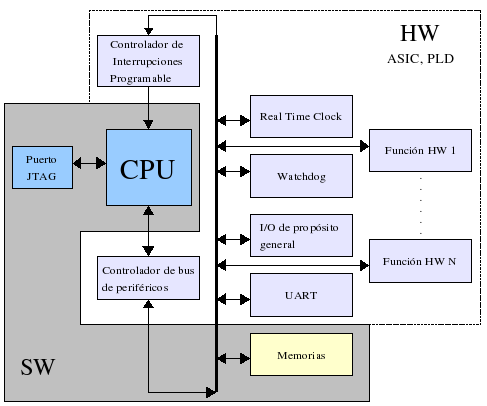
\includegraphics[scale=.6]{./images/ES_Architecture} \end{center}
  \caption{Arquitectura de un Sistema Embebido}\label{es_arch}
\end{figure} 


Podemos utilziar
\begin{itemize}
\item Componente HW y SW Integrado en un dispositivo semiconductor (SoC): En la actualidad existen muchas compa��as que fabrican procesadores de 32 bits integrados a una gran variedad de perif�ricos, lo cual simplifica el dise�o y reduce costos (menos componentes y menos �rea de circuito impreso) \footnote{http://www.sharpsma.com, http://www.atmel.com, http://www.cirrus.com, http://www.samsung.com, http://www.freescale.com, etc}.

\item Componente SW en un SoC y componente HW en una FPGA: Cuando no existen en el mercado SoC con la cantidad de perif�ricos requerida para una determinada aplicaci�n, es necesario recurrir a la utilizaci�n de dispositivos comerciales que implementen dicha operaci�n, en algunas ocaciones el perif�rico puede relizar funciones muy espec�ficas de modo que no existe en el mercado, la soluci�n es entonces implementar estos dispositivos en una FPGA, tambi�n se recomienda la utilizaci�n de FPGAs en sistemas que requieren una gran cantidad y variedad de perif�ricos ya que reduce la complejidad y costo del sistema.

\item Componente SW y HW en una FPGA: Esta es tal vez la opci�n m�s econ�mica y flexible, pero la de menor desempe�o, ya que al utilizar los recursos l�gicos de la FPGA para la implementaci�n del procesador (softcore) la lngitud de los caminos de interconexi�n entre los bloques l�gicos aumentan el retardo de las se�ales . Los procesadores \textit{softcore} m�s populares en la actualidad son:

  \begin{itemize}
  \item Microblaze de Xilinx\footnote{http://www.xilinx.com}
  \item Leon de Gaisler Research \footnote{http://www.gaisler.com/}
  \item LatticeMico32 de Lattice Semiconductors\footnote{http://www.latticesemi.com}
  \item OpenRisc \footnote{http://www.opencores.com}
  \end{itemize}
 
\end{itemize}


\section{Metodolog�a de Dise�o}

La Figura \ref{des_flow}, muestra un diagrama de flujo gen�rico para dise�o para sistemas embebidos {\cite{Cor05}}

\begin{figure}[H]
  \begin{center} 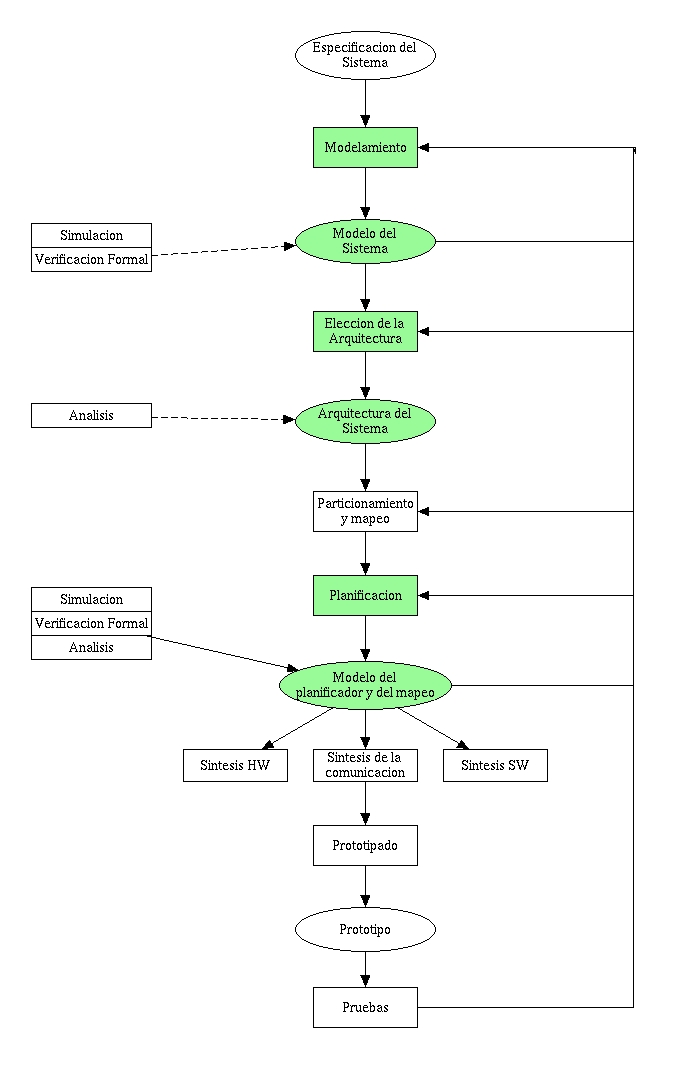
\includegraphics[scale=.55]{./images/design_flow} \end{center}
  \caption{Flujo de Dise�o de un Sistema Embebido}\label{des_flow}
\end{figure} 


El proceso comienza con la {\textit{especificaci\'on del sistema}}, en este punto se describe la funcionalidad y se definen las restricciones f\'{\i}sicas, el\'ectricas y econ\'omicas. Esta especificaci\'on debe ser muy general y no deben existir dependencias (tecnol\'ogicas, metodol\'ogicas) de ning\'un tipo, se suele utilizar lenguajes de alto nivel, como UML, C++. La especificaci\'on puede ser verificada a trav\'es de una serie de pasos de an\'alisis cuyo objetivo es determinar la validez de los algor\'{\i}tmos seleccionados, por ejemplo, determinar si el algoritmo siempre termina, los resultados satisfacen las especificaciones. Desde el punto de vista de la re-utilizaci\'on, algunas partes del funcionamiento global deben tomarse de una librer\'{\i}a de algor\'{\i}tmos existentes.

Una vez definidas las especificaciones del sistema se debe realizar un modelamiento que permita extraer de estas la funcionalidad. El modelamiento es crucial en el dise�o ya que de \'el depende el paso existoso de la especificaci\'on a la implementaci\'on. Es importante definir que modelo matem\'atico debe soportar el entorno de dise�o. Los modelos m\'as utilizados son: M\'aquinas de estados finitos, diagramas de flujos de datos, Sistemad de Eventos Discretos y Redes de Petri. Cada modelo posee propiedades matem\'aticas que pueden explotarse de forma eficiente para responder preguntas sobre la funcionalidad del sistema sin llevar a cabo dispendiosas tareas de verificaci\'on. \ Todo modelo obtenido debe ser verificado para comprobar que cumple con las restricciones del sistema.

Una vez se ha obtenido el modelo del sistema se procede a determinar su {\textit{arquitectura}}, esto es, el n\'umero y tipo de componentes y su inter-conexi\'on. Este paso no es m\'as que una exploraci\'on del espacio de dise�o en b\'usqueda de soluciones que permitan la implementaci\'on de una funcionalidad dada, y puede realizarse con varios criterios en mente: Costos, confiabilidad, viabilidad comercial.

Utilizando como base la arquitectura obtenida en el paso anterior las tareas del modelo del sistemas son mapeadas dentro de los componentes. Esto es,
asignaci\'on de funciones a los componentes de la arquitectura. Existen dos opciones a la hora de implementar las tareas o procesos:
\begin{enumerate}
  \item Implementaci\'on Software: La tarea se va a ejecutar en un procesador.
  \item Implementaci\'on Hardware: La tarea se va a ejecutar en un dispositivo l�gico programable.
\end{enumerate}

Para cumplir las especificaciones del sistema algunas tareas deben ser implementadas en Hardware, esto con el f\'{\i}n de no ocupar al procesador en tareas c\'{\i}clicas, un ejemplo t\'{\i}pico de estas tareas es la generaci\'on de bases de tiempos. La decisi\'on de que tareas se implementan en SW y que tareas se implementan en HW recibe el nombre de {\textit{particionamiento}}, esta selecci\'on es fuertemente dependiente de restricciones econ\'omicas y temporales.

Las tareas Software deben compartir los recursos que existan en el sistema (procesador y memoria), por lo tanto se deben hacer decisiones sobre el orden de ejecuci\'on y la prioridad de estas. Este proceso recibe el nombre de {\textit{planificaci\'on}}. En este punto del dise�o el modelo debe incluir informaci\'on sobre el mapeo, el particionamiento y la planificaci\'on del sistema.

Las siguientes fases corresponden a la implementaci\'on del modelo, para esto las tareas hardware deben ser llevadas al dispositivo elegido (ASIC o FPGA) y
se debe obtener el $''$ejecutable$''$ de las tareas software, este proceso recibe el nombre de {\textit{s\'{\i}ntesis}} HW y SW respectivamente, as\'{\i}
mismo se deben sintetizar los mecanismos de comunicaci\'on.

El proceso de prototipado consiste en la realizaci\'on f\'{\i}sica del sistema, finalmente el sistema f\'{\i}sico debe someterse a pruebas para verificar que se cumplen con las especificaciones iniciales.

Como puede verse en el flujo de dise�o existen realimentaciones, estas realimentaciones permiten depurar el resultado de pasos anteriores en el caso de no cumplirse las especificaciones iniciales


\section{Herramientas de Dise�o Software}

En el mercado existe una gran variedad de herramientas de desarrollo para Sistemas Embebidos, sin embargo, en este estudio nos centraremos en el uso de las herramientas de libre distribuci�n; esta elecci�n se debe a que la mayor�a de los productos comerciales utilizan el toolchain de GNU\footnote{http://www.gnu.org} internamente y proporcionan un entorno gr�fico para su f�cil manejo. Otro factor considerado a la hora de realizar nuestra elecci�n es el econ�mico, ya que la mayor�a de los productos comerciales son costosos y poseen soporte limitado. Por otro lado, el toolchain de GNU es utilizado ampliamente en el medio de los dise�adores de sistemas embebidos y se encuentra un gran soporte en m�ltiples foros de discusi�n (ver Figura \ref{tools}).

\begin{figure}[H]
  \begin{center} 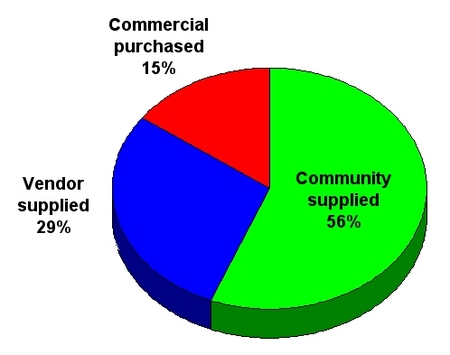
\includegraphics[scale=.7]{./images/embedded-linux-tool-trends-sm} \end{center}
  \caption{Tendencia de utilizaci�n de herramientas de desarrollo}\label{tools}
\end{figure}

\subsection{Componentes del \textit{GNU toolchain} }

\subsubsection{GNU binutils\cite{A1}}
Son una colecci�n de utilidades para archivos binarios y estan compuestas por:

\begin{itemize}
 \item  \textbf{addr2line} Convierte direcciones de un programa en nombres de archivos y n�meros de l�nea. Dada una direcci�n y un ejecutable, usa la informaci�n de depuraci�n en el ejecutabe para determinar que nombre de atchivo y n�mero de lpinea est� asociado con la direcci�n dada.
 \item  \textbf{ar} Esta utilidad crea, modifica y extrae desde ficheros. Un fichero es una colecci�n de otros archivos en una estructura que hace posible obtener los archivos individuales miembros del archivo. 
 \item  \textbf{as} Utilidad que compila la salida del compilador de C (GCC).
 \item  \textbf{c++filt} Este program realiza un mapeo inverso: Decodifica nombres de bajo-nivel en nombres a nivel de usuario, de tal forma que el linker pueda mantener estas funciones sobrecargadas (overloaded) ``from clashing''. 
 \item  \textbf{gasp} GNU Assembler Macro Preprocessor
 \item  \textbf{ld} El \textit{linker} GNU combina un n�mero de objetos y ficheros, re-localiza sus datos y los relaciona con referencias. Normalmente el �ltimo paso en la construcci�n de un nuevo programa compilado es el llamado a ld.
 \item  \textbf{nm} Realiza un listado de s�mbolos de archivos tipo objeto.
 \item  \textbf{objcopy} Copia los contenidos de un archivo tipo objeto a otro. \textit{objcopy} utiliza la librer�a GNU BFD para leer y escribir el archivo tipo objeto. Permite esccribibr el archivo destino en un formato diferente al del archivo fuente. 
 \item  \textbf{objdump} Despliega informaci�n sobre archivos tipo objeto. 
 \item  \textbf{ranlib} Genera un �ndice de contenidos de un fichero, y lo almacena en �l.
 \item  \textbf{readelf} Interpreta encabezados de un archivo ELF.
 \item  \textbf{size} Lista el tama�o de las secciones y el tama�o total de un archivo tipo objeto.
 \item  \textbf{strings} Imprime las secuencias de caracteres imprimibles de almenos 4 caracteres de longitud. 
 \item  \textbf{strip} Elimina todos los s�mbolos de un archivo tipo objeto.

\end{itemize}
 
\subsubsection{GNU Compiler Collection\cite{Wik}}
El \textit{GNU Compiler Collection} normalmente llamado GCC, es un grupo de compiladores de lenguajes de programaci�n producido por el proyecto GNU. Es el compilador standard para el software libre de los sistemas operativos basados en Unix y algunos propietarios como Mac OS de Apple.

\subsubsection{Lenguajes}
GCC soporta los siguientes lenguajes:
\begin{itemize}
 \item \textbf{ADA} 
 \item \textbf{C} 
 \item \textbf{C++} 
 \item \textbf{Fortran} 
 \item \textbf{Java} 
 \item \textbf{Objective-C} 
 \item \textbf{Objective-C++} 
\end{itemize}

\subsubsection{Arquitecturas}
\begin{itemize}
 \item \textbf{Alpha}
 \item \textbf{ARM}
 \item \textbf{Atmel AVR}
 \item \textbf{Blackfin}
 \item \textbf{H8/300}
 \item \textbf{System/370, System/390}
 \item \textbf{IA-32 (x86) and x86-64}
 \item \textbf{IA-64 i.e. the "Itanium"}
 \item \textbf{Motorola 68000}
 \item \textbf{Motorola 88000}
 \item \textbf{MIPS}
 \item \textbf{PA-RISC}
 \item \textbf{PDP-11}
 \item \textbf{PowerPC}
 \item \textbf{SuperH}
 \item \textbf{SPARC}
 \item \textbf{VAX}
 \item \textbf{Renesas R8C/M16C/M32C}
 \item \textbf{MorphoSys}
\end{itemize}
Como puede verse GCC soporta una gran cantidad de lenguajes de programaci�n, sin embargo, en el presente estudio solo lo utilizaremos como herramienta de compilaci�n para C y C++. Una caracter�stica de resaltar de GCC es la gran cantidad de plataformas que soporta, esto lo hace una herramienta Universal para el desarrollo de sistemas embebidos, el c�digo escrito en una plataforma (en un lenguaje de alto nivel) puede ser implementado en otra sin mayores cambios, esto elimina la dependencia entre el c�digo fuente y el HW\footnote{Esto recibe el nombre de re-utilizaci�n de c�digo}, lo cual no ocurre al utilizar lenguaje ensamblador. 

Por otro lado, el tiempo requerido para realizar aplicaciones utilizando C o C++ disminuye, ya que no es necesario aprender las instrucciones en assembler de una plataforma determinada; adem�s, la disponibilidad de librer�as de m�ltiples prop�sitos reduce a�n m�s los tiempos de desarrollo, permitiendo de esta forma tener bajos tiempos \textit{time to market} y reducir de forma considerable el costo del desarrollo. Una consecuencia de esto se refleja en el n�mero de desarrolladores en un grupo de trabajo, en la actualidad casi el 60\% de las empresas desarrolladoras de dispositivos embebidos tiene grupos con menos de 10 desarrolladores \ref{group}.


\begin{figure}[H]
  \begin{center} 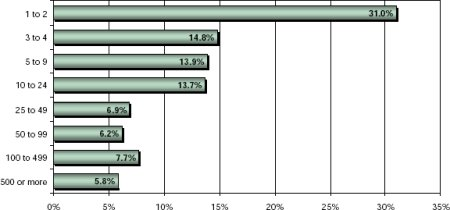
\includegraphics[scale=.2]{./images/vdc_embedded_dev_company_size} \end{center}
  \caption{N�mero promedio de desarrolladores por compa��a. Fuente Venture Development Corp}\label{group}
\end{figure}
 
\subsubsection{GNU Debugger}
El depurador oficial de GNU (GDB), es un depurador que al igual que GCC tiene soporte para m�ltiples lenguajes y plataformas. GDB permite al usuario monitorear y modificar las variables internas del programa y hacer llamado a funciones de forma independiente a la ejecuci�n normal del mismo. Adem�s, permite establecer sesiones remotas utilizando el puerto serie o TCP/IP. Aunque GDB no posee una interfaz gr�fica, se han desarrollado varios front-ends como DDD o GDB/Insight. A continuaci�n se muestra un ejemplo de una sesi�n con gdb.

\begin{lstlisting}[firstnumber=40]
GNU gdb Red Hat Linux (6.3.0.0-1.21rh)
Copyright 2004 Free Software Foundation, Inc.
GDB is free software, covered by the GNU General Public License, and you are
welcome to change it and/or distribute copies of it under certain conditions.
Type "show copying" to see the conditions.
There is absolutely no warranty for GDB.  Type "show warranty" for details.
This GDB was configured as "i386-redhat-linux-gnu"...Using host libthread_db 
library "/lib/libthread_db.so.1".

(gdb) run
Starting program: /home/sam/programming/crash
Reading symbols from shared object read from target memory...done.
Loaded system supplied DSO at 0xc11000
This program will demonstrate gdb

Program received signal SIGSEGV, Segmentation fault.
0x08048428 in function_2 (x=24) at crash.c:22
22         return *y;
(gdb) edit
(gdb) shell gcc crash.c -o crash -gstabs+
(gdb) run
The program being debugged has been started already.
Start it from the beginning? (y or n) y
warning: cannot close "shared object read from target memory": File in wrong format
`/home/sam/programming/crash' has changed; re-reading symbols.
Starting program: /home/sam/programming/crash
Reading symbols from shared object read from target memory...done.
Loaded system supplied DSO at 0xa3e000
This program will demonstrate gdb
24
Program exited normally.
(gdb) quit 
\end{lstlisting}



\subsubsection{C Libraries}
Adicionalmente es necesario contar con una librer�a que proporcione las librer�as standard de C: stdio, stdlib, math; las m�s utilizadas en sistemas embebidos son:

\begin{itemize}
 \item \textbf{glibc\footnote{http://www.gnu.org/software/libc/}} Es la librer�a C oficial del proyecto GNU. Uno de los inconvenientes al trabajar con esta librer�a en sistemas embebidos es que genera ejecutables de mayor tama�o que los generados a partir de otras librer�as, lo cual no la hace muy atractiva para este tipo de aplicaciones. 
 \item \textbf{uClibc\footnote{http://uclibc.org/}} Es una librer�a dise�ada especialmente para sistemas embebidos, es mucho m�s peque�a que \textbf{glibc}.
 \item \textbf{newlib\footnote{http://sources.redhat.com/newlib/}} Al igual que \textbf{uClibc}, est� dise�ada para sistemas embebidos. El t�pico ``Hello, world!'' ocupa menos de 30k en un entorno basado en newlib, mientras que en uno basado en glibc, puede ocupar 380k \cite{BG}. 
 \item \textbf{diet libc\footnote{http://www.fefe.de/dietlibc/}} Es una versi�n de \textit{libc} optimizada en tama�o, puede ser utilizada para crear ejecutables est�ticamente enlazados para linux en plataformas alpha, arm, hppa, ia64, i386, mips, s390, sparc, sparc64, ppc y x86\_64.
\end{itemize}


%%%%%%%%%%%%%%%%%%%%%%%%%%%%%%%%%%%%%%%%%%%%%%%%%%%%%%%%%%%%%%%%%%%%%%%%%%%%%%%%%%%%%%%%%%%%%%%%%%%%%%%%%%%%%%%%%%
%                                                     SECCION Obtenci�n y utilizaci�n del GNU toolchain
%%%%%%%%%%%%%%%%%%%%%%%%%%%%%%%%%%%%%%%%%%%%%%%%%%%%%%%%%%%%%%%%%%%%%%%%%%%%%%%%%%%%%%%%%%%%%%%%%%%%%%%%%%%%%%%%%%

\section{Desarrollo Software}

El primer paso en nuestro estudio consiste en tener una cadena de herramientas funcional que soporte la familia de procesadores a utilizar. La arquitectura sobre la cual realizaremos nuestro estudio inicial es la ARM (Advanced Risc Machines), ya que la m�s utilizada en la actualidad por los dise�adores de sistemas embebidos (ver figura \ref{arch}) y se encuentran disponibles una gran variedad de herramientas para esta arquitectura. Sin embargo, lo contenido en esta secci�n es aplicable a cualquier familia de procesadores soportada por la cadena de herrmientas GNU. Existen dos formas de obtener la cadena de herramientas GNU:

\begin{figure}
  \begin{center} 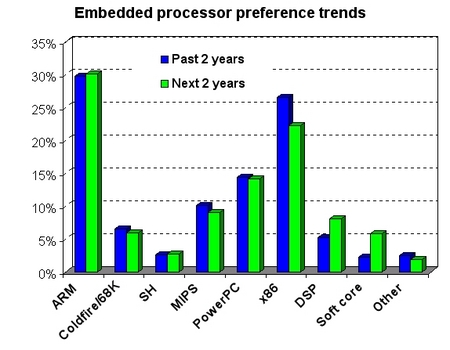
\includegraphics[scale=.8]{./images/embedded-processor-trends-sm} \end{center}
  \caption{Tendencia del mercado de procesadores para sistemas embebidos. Fuente:\cite{Lin05} }\label{arch}
\end{figure}

\begin{enumerate}
 \item Utilizar una distribuci�n precompilada: Esta es la via m�s r�pida, sin embargo, hay que tener cuidado al momento de instalarlas, ya que debe hacerse en un directorio con el mismo \textit{path} con el que fueron creadas. por ejemplo \textit{/usr/local/gnutools}; si esto no se cumple, las herramientas no funcionar�n de forma adecuada.
 \item Utilizar un script de compilaci�n: Existen disponibles en la red una serie de \textit{scripts} que permiten descargar, configurar, compilar e instalar la cadena de herramientas, la ventaja de utilizar este m�todo es que es posible elegir las versiones de las herramientas instaladas, al igual que el directorio de instalaci�n. En este estudio utilizaremos los \textit{scripts} creados por Dan Kegel \cite{DK06}.
\end{enumerate}

\subsection{Flujo de dise�o software}

En la figura \ref{toolchain_flow} se ilustra la secuencia de pasos que se realizan desde la creaci�n de un archivo de texto que posee el c�digo fuente que implementa la funcionalidad de una tarea software utilizando un lenguaje de alto nivel como C o C++, hasta su programaci�n en una memoria permanente en la plataforma f�sica. Los pasos necesarios para crear un archivo que pueda ser programado en dicha memoria son:

\begin{figure}
  \begin{center} 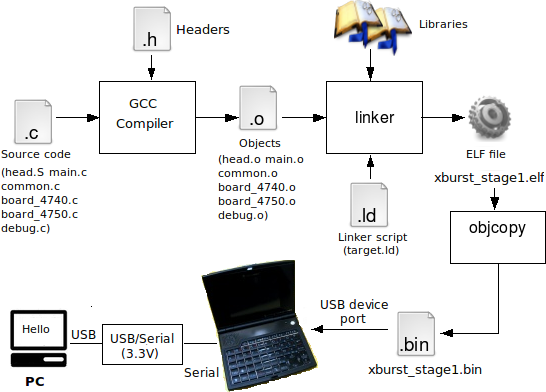
\includegraphics[scale=.6]{./images/SW_design_flow} \end{center}
  \caption{Tendencia del mercado de procesadores para sistemas embebidos. Fuente:\cite{Lin05} }\label{toolchain_flow}
\end{figure}


\begin{enumerate}
 \item \textbf{Escritura del c�digo fuente:} Creaci�n del c�digo fuente en cualquier editor de texto utilizando un lenguaje de alto nivel como C o C++.

 \item \textbf{Compilaci�n:} Utilizando un compilador (GCC en nuestro caso) se crea un \textit{objeto} que contiene las instrucciones en \textit{lenguaje de m�quina} del procesador a utilizar (uno diferente al que realiza la compilaci�n que normalmente es de la familia x86); en este punto el compilador solo busca en los encabezados (\textit{headers}) la definici�n de una determinada funci�n, esto es, la forma en que debe ser utilizada, el tipo de datos y el n�mero de par�metros con que debe ser invocada, por ejemplo, la funci�n \textit{printf} esta declarada en el archivo \textit{stdio.h} como: \textit{ int printf (const char *template, ...)}. Esta declaraci�n es utilizada por el compilador para verificar el correcto uso de esta funci�n.

 \item \textbf{Enlazado:} En esta etapa se realizan dos tareas: 
  \begin{enumerate} 
    \item Se enlazan los archivos tipo objeto del proyecto, junto con librer�as precompiladas para el procesador de la plataforma, si una determinada funci�n no es definida en ninguna de estas librer�as, el \textit{enlazador} generar� un error y no se generar� el ejecutable. 
    \item Se definen las posici�nes f�sicas de las secciones que componen el archivo ejecutable (tipo ELF), esto se realiza a trav�s de un link de enlazado en el que se define de forma expl�cita su localizaci�n.
  \end{enumerate}

 \item \textbf{Extracci�n del archivo de programaci�n} En algunas aplicaciones (cuando no se cuenta con un sistema operativo) es necesario extraer las secciones del ejecutable que residen en los medios de almacenamiento no vol�til, que como veremos m�s adelante representan el conjunto de instrucciones que debe ejecutar el procesador de la plataforma y las constantes del programa. Esto se realiza con la herramiento \textit{objcopy}, la cual, nos permite generar archivos en la mayor�a de los formatos soportados por los programadores de memorias y procesadores, como S19 e Intel Hex.

 \item \textbf{Descarga del programa a la plataforma}. Dependiendo de la plataforma existen varios m�todos para descargar el archivo de programaci�n a la memoria de la plataforma:
  \begin{enumerate}
    \item Utilizando un \textit{loader}: El \textit{loader} es una aplicaci�n que reside en un medio de almacenamiento no vol�til y permite la descarga de archivos utilizando el puerto serie, USB,  o una interfaz de red.
    \item Utilizando el puerto JTAG: El puerto JTAG (Joint Test Action Group) proporciona una interfaz capaz de controlar los registros internos del procesador, y de esta forma, acceder a las memorias de la plataforma y ejecutar un programa residente en una determinada posici�n de memoria.
  \end{enumerate}

 \item \textbf{Depuraci�n} Una vez se descarga la aplicaci�n a la plataforma es necesario someterla a una serie de pruebas con el f�n de probar su correcto funcionamiento. Esto se puede realizar con el depurador GNU (GDB) y una interfaz de comunicaci�n que puede ser un puerto serie, USB o un adaptador de red.
 
\end{enumerate}


\subsection{El formato \textbf{ELF}}

El formato ELF (\textit{Executable and Linkable Format}) Es un st�ndard para objetos, librer�as y ejecutables y es el formato que genera las herramientas GNU. Como puede verse en la figura \ref{elf1} est� compuesto por varias secciones (\textit{link view}) o segmentos (\textit{execution view}). Si un programador est� interesado en obtener informaci�n de secciones sobre tablas de s�mbolos, c�digo ejecutable espec�fico o informaci�n de enlazado din�mico debe utilizar \textit{link view}. Pero si busca informaci�n sobre segmentos, como por ejemplo, la localizaci�n de los segmentos \textit{text} o \textit{data} debe utilizar \textit{execution view}. El encabezado describe el layout del archivo, proporcionando informaci�n de la forma de acceder a las secciones \cite{MLH98}.

\begin{figure}
  \begin{center} \includegraphics[scale=.4]{./images/ELF_Link_exec1} \end{center}
  \caption{Formato ELF}\label{elf1}
\end{figure}

Las secciones pueden almacenar c�digo ejecutable, datos, informaci�n de enlazado din�mico, datos de depuraci�n, tablas de s�mbolos,comentarios, tablas de strings, y notas. Las secciones m�s importantes son las siguientes:

\begin{itemize}
 \item \textbf{.bss}            Datos no inicializados. (RAM)
 \item \textbf{.comment}        Informaci�n de la versi�n.
 \item \textbf{.data y .data1}  Datos inicializados.    (RAM)
 \item \textbf{.debug}          Informaci�n para depuraci�n simb�lica. 
 \item \textbf{.dynamic}        Informaci�n sobre enlace din�mico 
 \item \textbf{.dynstr}         Strings necesarios para el enlacedin�mico 
 \item \textbf{.dynsym}         Tabla de s�mbolos utilizada para enlace din�mico.
 \item \textbf{.fini}           C�digo de terminaci�n de proceso.
 \item \textbf{.init}           C�digo de inicializaci�n de proceso.
 \item \textbf{.line}           Informaci�n de n�mero de l�nea para depuraci�n simb�lica.
 \item \textbf{.rodata y .rodta1} Datos de solo-lectura (ROM)
 \item \textbf{.shstrtab}       Nombres de secciones.
 \item \textbf{.symtab}         Tabla de s�mbolos.
 \item \textbf{.text}           Instrucciones ejecutables (ROM)
\end{itemize}

Para aclarar un poco este concepto, escribamos una aplicaci�n sencilla:

\begin{lstlisting}
#include <stdio.h>

int global;
int global_1 = 1;

int main(void)
{
  int i;                                // Variable no inicializada
  int j = 2;                            // Variable inicializada
  for(i=0; i<10; i++){
    printf("Printing %d\n", i*j);       // Caracteres constantes
    j = j + 1;
    global   = i;
    global_1 = i+j;
  }
  return 0;
}
\end{lstlisting}

Generemos el objeto compil�ndolo con el siguiente comando:
\textit{arm-none-eabi-gcc -c hello.c}

Examinemos que tipo de secciones tiene este ejecutable
\textit{arm-none-eabi-readelf -S hello.o}

\begin{lstlisting}
Section Headers:
  [Nr] Name              Type            Addr     Off    Size   ES Flg Lk Inf Al
  [ 0]                   NULL            00000000 000000 000000 00      0   0  0
  [ 1] .text             PROGBITS        00000000 000034 00009c 00  AX  0   0  4
  [ 2] .rel.text         REL             00000000 000484 000020 08      9   1  4
  [ 3] .data             PROGBITS        00000000 0000d0 000004 00  WA  0   0  4
  [ 4] .bss              NOBITS          00000000 0000d4 000000 00  WA  0   0  1
  [ 5] .rodata           PROGBITS        00000000 0000d4 000010 00   A  0   0  4
  [ 6] .comment          PROGBITS        00000000 0000e4 00004d 00      0   0  1
  [ 7] .ARM.attributes   ARM_ATTRIBUTES  00000000 000131 00002e 00      0   0  1
  [ 8] .shstrtab         STRTAB          00000000 00015f 000051 00      0   0  1
  [ 9] .symtab           SYMTAB          00000000 000368 0000f0 10     10  11  4
  [10] .strtab           STRTAB          00000000 000458 00002b 00      0   0  1
Key to Flags:
  W (write), A (alloc), X (execute), M (merge), S (strings)
  I (info), L (link order), G (group), x (unknown)
  O (extra OS processing required) o (OS specific), p (processor specific)
\end{lstlisting}

La secci�n \textit{.text}, como se dijo anteriormente contiene las instrucciones ejecutables, por esta raz�n se marca como ejecutable \textit{``X''} en la columna \textit{Flg}. Es posible ver las instrucciones que se ejecutan en esta secci�n:

\textit{arm-none-eabi-objdump -d -j .text hello.o}

\begin{lstlisting}
00000000 <main>:
   0:   e92d4800        stmdb   sp!, {fp, lr}
   4:   e28db004        add     fp, sp, #4      ; 0x4
   8:   e24dd008        sub     sp, sp, #8      ; 0x8
   c:   e3a03002        mov     r3, #2  ; 0x2
  10:   e50b3008        str     r3, [fp, #-8]
  14:   e3a03000        mov     r3, #0  ; 0x0
  18:   e50b300c        str     r3, [fp, #-12]
  1c:   ea000013        b       70 <main+0x70>
  20:   e51b200c        ldr     r2, [fp, #-12]
  24:   e51b3008        ldr     r3, [fp, #-8]
  28:   e0030392        mul     r3, r2, r3
  2c:   e59f005c        ldr     r0, [pc, #92]   ; 90 <.text+0x90>
  30:   e1a01003        mov     r1, r3
  34:   ebfffffe        bl      0 <printf>
  38:   e51b3008        ldr     r3, [fp, #-8]
  3c:   e2833001        add     r3, r3, #1      ; 0x1
  40:   e50b3008        str     r3, [fp, #-8]
  44:   e59f2048        ldr     r2, [pc, #72]   ; 94 <.text+0x94>
  48:   e51b300c        ldr     r3, [fp, #-12]
  4c:   e5823000        str     r3, [r2]
  50:   e51b200c        ldr     r2, [fp, #-12]
  54:   e51b3008        ldr     r3, [fp, #-8]
  58:   e0822003        add     r2, r2, r3
  5c:   e59f3034        ldr     r3, [pc, #52]   ; 98 <.text+0x98>
  60:   e5832000        str     r2, [r3]
  64:   e51b300c        ldr     r3, [fp, #-12]
  68:   e2833001        add     r3, r3, #1      ; 0x1
  6c:   e50b300c        str     r3, [fp, #-12]
  70:   e51b300c        ldr     r3, [fp, #-12]
  74:   e3530009        cmp     r3, #9  ; 0x9
  78:   daffffe8        ble     20 <main+0x20>
  7c:   e3a03000        mov     r3, #0  ; 0x0
  80:   e1a00003        mov     r0, r3
  84:   e24bd004        sub     sp, fp, #4      ; 0x4
  88:   e8bd4800        ldmia   sp!, {fp, lr}
  8c:   e12fff1e        bx      lr
\end{lstlisting}

La secci�n \textit{.data} mantiene las variables inicializadas, y contiene:
 
\textit{arm-none-eabi-objdump -d -j .data hello.o}
 
\begin{lstlisting}
00000000 <global_1>:
   0:   01 00 00 00
\end{lstlisting}

Como vemos, la secci�n \textit{.data} contiene \'unicamente el valor de inicializaci\'on de la variable \textit{global\_1} (1) y no muestra informaci�\'on acerca de la variable \textit{j}, esto se debe a que la informaci\'on est\'a en el \textit{stack} del proceso. Si observamos el contenido de la secci�n \textit{.text} observamos que esta variable es asignada en tiempo de ejecuci�n, en la l�nea \textit{0c:} se ve la asignaci�n de esta variable.

\begin{lstlisting}
0c:   e3a03002        mov     r3, #2  ; 0x2 
10:   e50b3008        str     r3, [fp, #-8]
\end{lstlisting}


La secci�n \textit{.bss} mantiene la informaci\'on de las variables no incializadas (En Linux todas las variables no inicializadas, se inicializadan en cero):

\textit{arm-none-eabi-objdump -d -j .bss hello}
 
\begin{lstlisting}
000145c4 <global>:
    145c4:       00000000
\end{lstlisting}
   
 
La secci�n \textit{.rodata} mantiene los datos que no cambian durante la ejecuci�n del programa, es decir, de solo lectura, si examinamos esta secci�n obtenemos:
 
\textit{hexdump -C hello.o | grep -i 000000d0} (la secci�n \textit{.rodata} comienza en la posici�n de memoria 0xd4)
 
  
\begin{lstlisting}
000000d0  01 00 00 00 50 72 69 6e  74 69 6e 67 20 25 64 0a  |....Printing %d.|
000000e0  00 00 00 00 00 47 43 43  3a 20 28 43 6f 64 65 53  |.....GCC: (CodeS|
\end{lstlisting}
 
En el contenido de esta secci�n aparece la cadena de caracteres \textit{Printing \%d\\n}, es decir, los datos que no cambian durante la ejecuci�n.


\subsection{Herramienta de compilaci�n make}
Como pudo verse en la secci�n es necesario realizar una serie de pasos para poder descargar una aplicaci�n a una plataforma embebida. Debido a que las herramientas GNU solo poseen entrada por consola, es necesario esribir una serie de comandos cada vez que se realiza un cambio en el c�digo fuente, lo cual resulta poco pr�ctico. Para realizar este proceso de forma autom�tica se cre� la herramienta \textit{make}, la cual recibe como entrada un archivo que normalmente tiene el nombre \textit{Makefile} o \textit{makefile} y determina que archivos han sido modificados desde la �ltima compilaci�n y ejecuta los comandos necesarios para recompilarlos. Un ejemplo de este tipo de archivo se muestra a continuaci�n:

\begin{lstlisting}[numbers=left]
SHELL = /bin/sh

basetoolsdir = /home/at91/gcc-3.4.5-glibc-2.3.6/arm-softfloat-linux-gnu
bindir  = ${basetoolsdir}/bin
libdir  = ${basetoolsdir}/lib/gcc/arm-softfloat-linux-gnu/3.4.5

CC      = arm-softfloat-linux-gnu-gcc 
AS      = arm-softfloat-linux-gnu-as 
LD      = arm-softfloat-linux-gnu-ld
OBJCOPY = arm-softfloat-linux-gnu-objcopy

CFLAGS  =-mcpu=arm920t -I. -Wall
LDFLAGS =-L${libdir} -l gcc

OBJS = \
	main.o 			\
	debug_io.o 		\
	at91rm9200_lowlevel.o 	\
	p_string.o

ASFILES = arm_init.o

LIBS=${libdir}/

all: hello_world 

hello_world: ${OBJS} ${ASFILES} ${LIBS}
	${LD} -e 0 -o hello_world.elf -T linker.cfg ${ASFILES} ${OBJS} ${LDFLAGS}
	${OBJCOPY} -O binary hello_world.elf hello_world.bin

clean:
	rm -f *.o *~ hello_world.*

PREPROCESS.c = $(CC) $(CPPFLAGS) $(TARGET_ARCH) -E -Wp,-C,-dD,-dI

%.pp : %.c FORCE
	$(PREPROCESS.c) $< > $@
\end{lstlisting}

En las l�neas 3-5 se definen algunas variables globales que ser�n utilizadas a lo largo del archivo; en las l�neas 7 - 10 se definen las herramientas de compilaci�n a utilizar, espec�ficamente el compilador C (CC), el ensamblador (AS), el enlazador (LD) y la utilidad objcopy. A partir de la l�nea 15 se definen los objetos que forman parte del proyecto, en este caso: \textit{main.o, debug\_io.o, at91rm9200\_lowlevel.o y p\_string.o}; en la l�nea 21 se definen los archivos en assembler que contiene el proyecto, para este ejemplo \textit{arm\_init.o}. Las l�neas 12 y 13 definen dos variables especiales que se pasan directamente al compilador C (CFLAGS) y al enlazador (LDFLAGS) y definen par�metros de comportamiento de estas herramientas.

\begin{lstlisting}
CFLAGS  =-mcpu=arm920t -I. -Wall
\end{lstlisting}

El par�metro \textit{-mcpu} le indica al compilador C para arquitecturas \textit{ARM} que utilice la familia \textit{arm920}; el par�metro \textit{-I} le indica un directorio donde puede buscar los encabezados, en este caso el caracter "." le indica que busque en el mismo sitio donde se encuentran los archivos fuente; el par�metro \textit{-Wall} le indica que imprima todos los mensajes de errores y advertencias.

\begin{lstlisting}
LDFLAGS =-L${libdir} -l gcc
\end{lstlisting}

El par�metro \textit{-L} le indica al enlazador la ruta del directorio donde se encuentran las librer�as, en este ejemplo apunta a la variable textit{libdir} que se encuentra declarado como \textit{\${basetoolsdir}/lib/gcc/arm-softfloat-linux-gnu/3.4.5}; el par�metro \textit{-l} le indica al enlazador que debe utilizar la librer�a \textit{gcc} que se encuentra en el directorio definido previamente. En realidad el archivo de la librer�a tienen el nombre \textit{libgcc.a}, pero como todas las librer�as tienen el nombre \textit{libXXXX.a} se eliminan el encabezado y la extensi�n del archivo.


En las l�neas 25, 27 y 31 aparecen unas etiquetas de la forma: \textit{nombre:} estos labels permiten ejecutar de forma independiente el conjunto de instrucciones asociadas a ellas, por ejemplo, si se ejecuta:
\\ \bigskip
\textit{make clean}\\ \bigskip
make ejecutar� el comando:\\ \bigskip
\textit{rm -f *.o *~ hello\_world.*} 

Observemos los comandos asociados a la etiqueta \textit{hello\_world:} En la misma l�nea aparecen \textit{\${OBJS} \${ASFILES} \${LIBS}} esto le indica a la herramienta \textit{make} que antes de ejecutar los comandos asociados a este label, debe realizar las acciones necesarias para generar \textit{\${OBJS} \${ASFILES} \${LIBS}} o lo que es lo mismo: \textit{main.o, debug\_io.o, at91rm9200\_lowlevel.o, p\_string.o, arm\_init.o y libgcc.a}. Para esto, \textit{make} tiene predefinidas una serie de reglas para compilar los archivos .c la regla es de la forma:

\begin{lstlisting}

.c.o:
        $(CC) $(CFLAGS) -c $<
.c:
        $(CC) $(CFLAGS) $@.c $(LDFLAGS) -o $@
 
\end{lstlisting}

Lo cual le indica a la herramienta make que para generar un archivo \textit{.o} a partir de uno \textit{.c} es necesario ejecutar \textit{\$(CC) \$(CFLAGS) -c \$<}; de aqui la importancia de definir bien la variable de entorno \textit{CC} cuando trabajamos con compiladores cruzados\footnote{Un compilador cruzado genera c�digo para una plataforma diferente en la que se est� ejecutando, por ejemplo, genera ejecutables para ARM pero se ejecuta en un x86}. Hasta este punto al ejecutar el comando: \textit{make hello\_world}, \textit{make} realizar�a las siguientes operaciones: \\

\begin{lstlisting}
arm-softfloat-linux-gnu-gcc  -mcpu=arm920t -I. -Wall   -c -o main.o main.c
arm-softfloat-linux-gnu-gcc  -mcpu=arm920t -I. -Wall   -c -o debug_io.o debug_io.c
arm-softfloat-linux-gnu-gcc  -mcpu=arm920t -I. -Wall   -c -o at91rm9200_lowlevel.o at91rm9200_lowlevel.c
arm-softfloat-linux-gnu-gcc  -mcpu=arm920t -I. -Wall   -c -o p_string.o p_string.c
arm-softfloat-linux-gnu-as    -o arm_init.o arm_init.s
\end{lstlisting}

En las l�neas 28 se realiza el proceso de enlazado; al \textit{enlazador} se le pasan los par�metros:
\begin{itemize}
 \item \textbf{-e 0}: Punto de entrada , utiliza la direcci�n de memoria 0 como punto de entrada.
 \item \textbf{-o hello\_world.elf}: Nombre del archivo de salida \textit{hello\_world}
 \item \textbf{-T linker.cfg}: Utilice el archivo de enlace \textit{linker.cfg} para definir las posiciones de memoria de las secciones del ejecutable.
 \item \textbf{\${ASFILES} \${OBJS} \${LDFLAGS}}: Lista de objetos y librer�as para crear el ejecutable.
\end{itemize}

En la l�nea 29 se utiliza la herramienta \textit{objcopy} para generar un archivo binario (\textit{-O binary}) con la informaci�n necesaria para cargar en una memoria no vol�til.


\subsection{Archivo de enlace}

Como vimos anteriormente, el enlazador o \textit{linker} es el encargado de agrupar todos los archivos objeto \textit{.o}, y las librer�as necesarias para crear el ejecutable, adicionalmente, permite definir donde ser�n ubicados los diferentes segmentos del archivo ELF en un archivo de enlace \textit{linker script}. De esta forma podemos ajustar el ejecutable a plataformas con diferentes configuraciones de memoria, lo que proporciona un grado mayor de flexibilidaad de la cadena de herramientas GNU.  Cuando se dispone de un sistema operativo como Linux no es necesario definir este archivo, ya que el sistema operativo se encarga del manejo de las diferentes secciones, sin embargo, es necesario tenerlo presente ya que como veremos m�s adelante existe un momento en el que el sistema operativo no ha sido cargado en la plataforma y las aplicaciones que se ejecuten deben proporcionar esta informaci�n. A continuaci�n se muestra un ejemplo de este archivo:

\begin{lstlisting}
 /* identify the Entry Point  (_vec_reset is defined in file crt.s)  */
ENTRY(_vec_reset)

/* specify the memory areas  */
MEMORY 
{
    flash : ORIGIN = 0,          LENGTH = 256K    /* FLASH EPROM          */
    ram   : ORIGIN = 0x00200000, LENGTH = 64K     /* static RAM area      */
}

/* define a global symbol _stack_end */
_stack_end = 0x20FFFC;

/* now define the output sections  */
SECTIONS
{
  . = 0;            /* set location counter to address zero  */
  .text :           /* collect all sections that should go into FLASH after startup  */
  {
    *(.text)        /* all .text sections (code)  */
    *(.rodata)      /* all .rodata sections (constants, strings, etc.)  */
    *(.rodata*)     /* all .rodata* sections (constants, strings, etc.)  */
    *(.glue_7)      /* all .glue_7 sections  (no idea what these are) */
    *(.glue_7t)     /* all .glue_7t sections (no idea what these are) */
    _etext = .;     /* define a global symbol _etext just after the last code byte */
  } >flash          /* put all the above into FLASH */

  .data :           /* collect all initialized .data sections that go into RAM  */ 
  {
    _data = .;      /* create a global symbol marking the start of the .data section  */
    *(.data)        /* all .data sections  */
    _edata = .;     /* define a global symbol marking the end of the .data section  */
  } >ram AT >flash  /* put all the above into RAM (but load the LMA initializer copy into FLASH)  */

  .bss :            /* collect all uninitialized .bss sections that go into RAM  */
  {
    _bss_start = .; /* define a global symbol marking the start of the .bss section */
    *(.bss)         /* all .bss sections  */
  } >ram            /* put all the above in RAM (it will be cleared in the startup code */
  . = ALIGN(4);     /* advance location counter to the next 32-bit boundary */
  _bss_end = . ;    /* define a global symbol marking the end of the .bss section */
}
_end = .;           /* define a global symbol marking the end of application RAM */
\end{lstlisting}

En las primeras l�neas del archivo aparece la declaraci�n de las memorias de la plataforma, en este ejemplo tenemos una memoria RAM de 64kB que comienza en la posici�n de memoria 0x00200000 y una memoria flash de 256k que comienza en la posici�n 0x0. A continuacion se definen las secciones y el lugar donde ser�n almacenadas; En este caso, las secciones \textit{.text} (c�digo ejecutable) y \textit{.rodata} (datos de solo lectura) se almacenan en una memoria no vol�til la flash. Cuando el sistema sea energizado el procesador ejecutar� el c�digo almacenado en su memoria no vol�til. Las secciones \textit{.data} (variables inicializadas) y \textit{.bss} (variables no inicializadas) se almacenar�n en la memoria vol�til RAM, ya que el acceso a las memorias no vol�tiles son m�s lentas y tienen ciclos de lectura/escritura finitos.

\section{Herramientas hardware}
En esta subsecci�n se realizar� una breve descripci�n de los dispositivos semiconductores m�s utilizados para la implementaci�n de dispositivos digitales, esto, con el f�n de determinar el estado actual de la industria de los semiconductores y entender los componentes b�sicos con los que se pueden implementar dispositivos digitlaes modernos.

\subsection{SoC}

La Figura \ref{at91rm} muestra la arquitectura de un SoC actual, espec�ficamente del AT91RM920 de Atmel. En este diagrama podemos observar el n�cleo central un procesador ARM920T de 180MHz y los perif�ricos asociados a �l. En la actualidad podemos encontrar una gran variedad de SoC dise�ados para diferentes aplicaciones: Multimedia, Comunicaciones, Asistentes Digitales; los perif�ricos incluidos en cada SoC buscan minimizar el n�mero de componentes externos, y de esta forma reducir los costos. Este SoC en particular fu� uno de los primeros que dise�o ATMEL y est� enfocado a tareas en las que se requiere una conexi�n de red. La arquitectura de estos SoC evoluciona muy r�pido acomod�ndose a los requerimientos de nuevas aplicaciones, b�sicamente, los cambios se producen en la velocidad del procesador central y la adici�n de perif�ricos que permiten el control directo de nuevos perif�ricos, como por ejemplo, la adici�n de controladores de pantallas de cristal l�quido o salidas de video. Dentro de estos perif�ricos encontramos:
 \begin{itemize}
  \item Controlador para memorias: NAND flash, DataFlash, SDRAM, DDR, SD/MMC
  \item Puertos USB host o device.
  \item Puerto I2C
  \item Interfaz Ethernet 10/100.
  \item Interfaz high speed USB 2.0
  \item Puertos SPI.
  \item Puertos seriales (RS232).
  \item Soporte JTAG.
  \item Interf�z de Bus externo (EBI).
  \item Controlador de LCD.
  \item Driver de video.
  \item Tarjetas de sonido.
 \end{itemize}

\begin{figure}
  \begin{center} 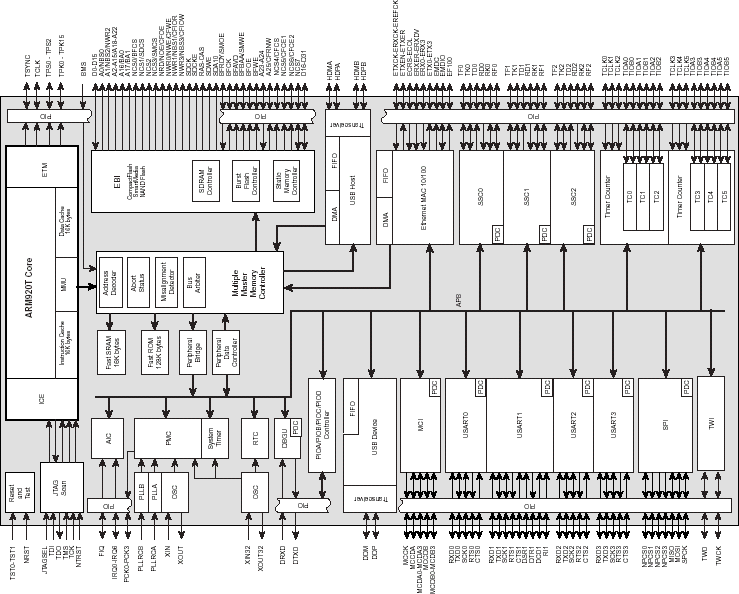
\includegraphics[scale=.7]{./images/at91rm9200} \end{center}
  \caption{SoC AT91RM9200 fuente: Hoja de Especificaciones AT91RM9200, ATMEL} \label{at91rm}
\end{figure}

Existen una serie de perif�ricos que son indispensables en todo Sistema Embebido, los cuales facilitan la programaci�n de aplicaciones y la depuraci�n de las mismas. Uno de los m�s importantes y que est�n presentes en todos los SoC actuales es el controlador de memorias, este perif�rico permite controlar los medios de almecenamiento que son vitales para la correcta oepraci�n del dispositivo, a continuaci�n se hace un breve recuento de las memorias disponibles para el desarrollo de aplicaciones embebidas.

\subsection{Memorias Vol�tiles}

Como se estudi� anteriormente existen secciones de un ejecutable que deben ser almacenadas en memorias vol�tiles o en memorias no vol�tiles. Debido a esto, la mayor�a de los SoC incluyen perif�ricos dedicados a controlar diferentes tipos de memoria, las memorias vol�tiles son utilizadas como memoria de acceso aleatorio (RAM) gracias a su bajo tiempo de accesso y al ilimitado n�mero de ciclos de lectura/escritura. 

\subsubsection{memoria SDRAM}
El tipo de memoria m�s utilizado en los sistemas embebidos actuales es la memoria SDRAM; la cual est� organizada como una matriz de celdas, con un n�mero de bits dedicados al direccionamiento de las filas y un n�mero dedicado a direccionar columnas (ver Figura \ref{sdram_basics}).

\begin{figure}
  \begin{center} 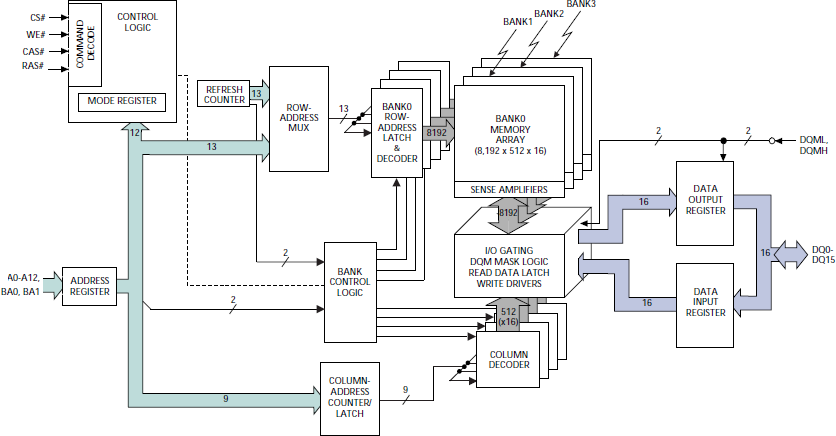
\includegraphics[scale=.6]{./images/sdram_basics} \end{center}
  \caption{Diagrama de Bloques de una memoria SDRAM fuente: Hoja de Especificaciones MT48LC16M16, Micron Technology} \label{sdram_basics}
\end{figure}

Una celda de memoria SDRAM esta compuesta por un transistor y un condensador; el transistor suministra la carga y el condensador almacena el estado de cada celda, esta carga en el condensador desaparece con el tiempo, raz�n por la cual es necesario recargar estos condensadores peri�dicamente, este proceso recibe el nombre de \textit{Refresco}. Un ciclo de refresco es un ciclo especial en el que no se escribe ni se lee informaci�n, solo se recargan los condensadores para mantener la informaci�n.

Un ejemplo simplificado de una operaci�n de lectura es el siguiente: Una posici�n de memoria se determina colocando la direcci�n de la fila y la de la columna en las l�neas de direcci�n de fila y columna respectivamente, un tiempo despu�s el dato almacenado aparecer� en el bus de datos. El procesador coloca la direcci�n de la fila en el bus de direcciones y despu�s activa la se�al \textit{RAS} (Row Access Strobe). Despu�s de un retardo de tiempo predeterminado para permitir que el circuito de la SDRAM capture la direcci�n de la fila, el procesador coloca la direcci�n de la columna en el bus de direcciones y activa la se�al \textit{CAS} (Column Access Strobe). El perif�rico que controla la SDRAM est� encargado de garantizar los ciclos de refresco de acuerdo con los requerimientos de la SDRAM \cite{CH06}.

\subsection{Memorias No Vol�tiles}
La memorias no vol�tiles almacenan por largos per�odos de tiempo la informaci�n necesaria para la operaci�n de un Sistema Embebido, pueden ser vistos como discos duros de estado s�lido. Existen dos tipos de memoria las NOR y las NAND; las dos poseen la capacidad de ser escritas y borradas utilizando control de software, con lo que no es necesario utilizar programadores externos y pueden ser modificadas una vez sean instaladas en el circuito impreso. Una desventaja de estas memorias es que los tiempos de escritura y borrado son muy largos en comparaci�n con los de las memorias RAM y que presentan un n�mero finito de ciclos de borrado y exritura.

\subsubsection{Memorias NOR}

Las memorias NOR poseen buses de datos y direcci�n, con lo que es posible acceder de forma f�cil a cada byte almacenado en ella. Los bits almacenados pueden ser cambiados de 0 a 1 utilizando el control de software un byte a la vez, sin embargo, para cambiar un bit de 1 a 0 es necesario borrar una serie de unidades de borrado que reciben el nombre de bloques, lo que reduce el tiempo de borrado de la memoria. Debido a que el borrado y escritura de una memoria ROM se puede realizar utilizando el control software (ver Figura \ref{nor_prog}) no es necesario contar con un perif�rico especializado para su manejo. Las memorias NOR son utilizadas en aplicaciones donde se necesiten altas velocidades de lectura y baja densidad, debido a que los tiempos de escritura y lectura son muy grandes, se utilizan como memorias ROM.

\begin{figure}
  \begin{center} \includegraphics[scale=.6]{./images/nor_prog} \end{center}
  \caption{Ciclos de escritura y borrado de una memoria flash NOR} \label{nor_prog}
\end{figure}

\subsubsection{Memorias NAND}

Las memorias NAND disminuyen los tiempos de escritura y aumentan la capacidad de almacenamiento, ideales para aplicaciones donde se requiera almacenamiento de informaci�n. Adicionalmente las memorias NAND consumen menos potencia que las memorias NAND, por esta raz�n este tipo de memorias son utilizadas en casi todos los dispositivos de almacenamiento modernos como las memorias SD y las memorias USB, los cuales integran una memoria NAND con un circuito encargado de controlarlas e implementar el protocolo de comunicaci�n. A diferencia de las flash tipo NOR, los dispositivos NAND se acceden de forma serial utilizando interfaces complejas; su operaci�n se asemeja a un disco duro tradicional. Se accede a la informaci�n utilizando bloques (m�s peque�os que los bloques NOR). Los ciclos de escritura de las flash NAND son mayores en un orden de magnitud que los de las memorias NOR.

Un problema al momento de trabajar con las memorias tipo NAND es que requieren el uso de un \textit{manejo de bloques defectuosos}, esto es necesario ya que las celdas de memoria pueden da�arse de forma espont�nea durante la operaci�n normal. Debido a esto se debe tener un determinado n�mero de bloques que se encargen de almacenar tablas de mapeo para manejar los bloques defectuosos; o puede hacerse un chequeo en cada inicializaci�n del sistema de toda la RAM para actualizar esta lista de sectores defectuosos. El algoritmo de ECC (Error-Correcting Code) debe ser cap�z de corregir errores tan peque�os como un bit de cada 2048 bits, hasta 22 bits de cada 2048. Este algor�tmo es capaz de detectar bloques defectuosos en la fase de programac��n comparando la informaci�n almacenada con la que debe ser almacenada (verificaci�n), si encuentra un error marca el bloque como defectuoso y utiliza un bloque sin defactos para almacenar la informaci�n.


La tabla \ref{flash_comp} resume las principales caracter�sticas de los diferentes tipos de memoria flash y muestra sus aplicaciones t�picas.

\begin{center}
  \begin{table}[ht]
  \begin{tabular}{|l|c|c|c|}
    \hline
                           & \textbf{SLC NAND} & \textbf{MLC NAND}  & MLC NOR         \\ \hline
     Densidad              & 512Mbits - 4GBits & 1Gbits - 16GBits   & 16MBits - 1GBit \\ \hline
     Velocidad de Lectura  & 24MB/s            & 18.6MB/s           & 103MB/s         \\ \hline
     Velocidad de escritura& 8 MB/s            & 2.4MB/s            & 0,47MB/s        \\ \hline
     Tiempo de borrado     & 2ms               & 2ms                & 900ms           \\ \hline
     Interfaz              & Acceso Indirecto  & Acceso Indirecto   & Acceso Aleatorio\\ \hline
     Aplicaci�n            & Almacenamiento    & Almacenamiento     & Solo lectura    \\ \hline
  \end{tabular}
  \caption{Cuadro de comparaci�n de las memorias flash NAND y NOR} \label{flash_comp} 
  \end{table}
\end{center}

Adicionalmente, se encuentran dispoibles las memorias DATAFLASH, estos dispositivos son b�sicamente una memoria flash tipo NOR con una interfaz SPI, permite una velocidad de lectura de  hasta 66MHz utilizando solamente 4 pines para la comunicaci�n con el procesador.


		%INTRODUCCION (CAIN - FES)
%\chapter{Sistema en un Chip (SoC)}

En esta secci�n estudiaremos la arquitectura b�sica de un SoC moderno, componentes, funcionamiento, programaci�n y operaci�n. Como se mencion� anteriormente, la tendencia actual de la industria de los semiconductores es integrar en un solo dispositivo las funcionalidades necesarias para la implementaci�n de dispositivos digitales modernos. Esto es posibe gracias a los grandes avances en las t�cnicas de fabricaci�n de circuitos integrados y a la demanda de nuevas caracter�sticas exigidas por los fabricantes de dispositivos digitales de consumo masivo como tel�fonos celulares, PDAs, consolas de juegos y reproductores multimedia. Para utilizar estos avances tecnol�gicos es necesario conocer su arquitectura, principio de funcionamiento, programaci�n e implementaci�n, para esto, se estudiar�n dos proyectos abiertos que implementan un SoC en un PLD utilizando lenguaje de descripci�n de hardware y herramientas GNU; proporcionan el c�digo fuente, lo que permite un estudio profundo de su arquitectura. El proyecto \textit{Plasma} \cite{SR08} y el proyecto Mico32\cite{LSC08}.


\section{Arquitectura}

Un SoC, integra un conjunto de perif�ricos, memorias y una o varias unidades de procesamiento (CPUs) en un solo chip, lo cual facilita el desarrollo de aplicaciones. Comercialmente encontramos una gran variedad de configuraciones CPU - perif�ricos, dependiendo de la aplicaci�n; dentro de los m�s comunes se encuentran: controladores de memorias externas (NOR, NAND, SDRAM, DDR), puertos de comunicaci�n (I2C, SPI), puerto de depuraci�n (UART), timers, reloj de tiempo real, codecs de audio, controladores de LCD, controladores de red, controlador de puerto USB host, controlador para sensores de im�genes, etc. La figura \ref{min_soc_arch} muestra una arquitectura de un SoC sencillo con los componentes necesarios para implementar tareas simples.


\begin{figure}
  \begin{center} 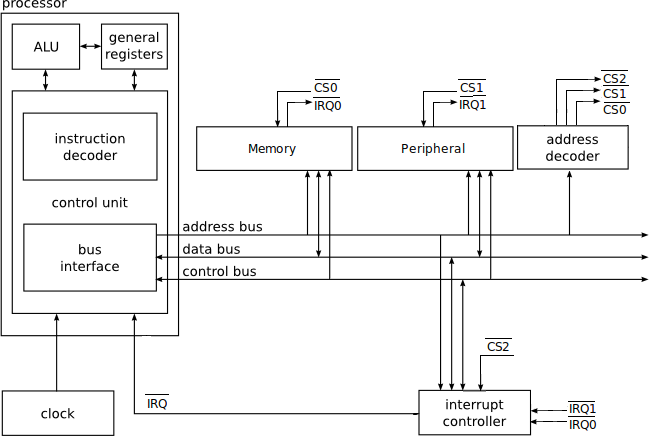
\includegraphics[scale=.6]{./images/Computer-simple} \end{center}
  \caption{Arquitectura m�nima de un SoC}\label{min_soc_arch}
\end{figure}

\subsubsection{Unidad de Procesamiento Central (CPU)}

La unidad de procesamiento central (CPU), como su nombre lo indica, est� encargada de centralizar las tareas del sistema coordinando las acciones de los perif�ricos. Puede ser vista como una m�quina de estados programable que controla un camino de datos compuesto por bloques aritm�ticos, l�gicos y un banco de registros. Cada CPU es capaz de realizar una serie de operaciones sobre variables almacenadas en el banco de registros, estas operaciones reciben el nombre de \textit{conjunto de instrucciones}. El programador utiliza estas instrucciones para hacer que la CPU realice una funci�n espec�fica, indicandole paso a paso donde debe leer la informaci�n, como procesarla y como entregar el resultado. A Esta funci�n se le conoce con el nombre de programa o tarea Software.


\subsubsection{Perif�ricos}
Los perif�ricos proporcionan la comunicaci�n con el exterior, permiten el ingreso, almacenamiento y procesamiento de la informaci�n


	%MAQUINAS ESTADOS ALGORITMICAS (FES)
%%%%%%%%%%%%%%%%%%%%%% chapter.tex %%%%%%%%%%%%%%%%%%%%%%%%%%%%%%%%%
%
% sample chapter
%
% Use this file as a template for your own input.
%
%%%%%%%%%%%%%%%%%%%%%%%% Springer-Verlag %%%%%%%%%%%%%%%%%%%%%%%%%%
%\motto{Use the template \emph{chapter.tex} to style the various elements of your chapter content.}
\chapter{M�quinas de Estado Algor�tmicas (ASM)}
\label{ASMChapter} % Always give a unique label
% use \chaptermark{}
% to alter or adjust the chapter heading in the running head

\begin{svgraybox}
\abstract{La l�gica de transfer.}
\end{svgraybox}

\section{Introducci�n}
	%LM32 (CAIN)   
%\include{Chapter4/chapter4}	%SO RTOS (DM)	
%\include{Chapter5/chapter5}	%LINUX (JRB)
%%%%%%%%%%%%%%%%%%%%%% chapter.tex %%%%%%%%%%%%%%%%%%%%%%%%%%%%%%%%%
%% At the end, it won't supposed to have
%% %! For Obs
%% %R For bib
%%%%%%%%%%%%%%%%%%%%%%%% Springer-Verlag %%%%%%%%%%%%%%%%%%%%%%%%%% 
%\motto{Use the template \emph{chapter.tex} to style the various elements of your chapter content.}
\chapter{Herramientas libres para construir proyectos Hardware-Software}
\label{intro} % Always give a unique label
%

\begin{svgraybox}
\abstract{En los anteriores cap�tulos se ha tratado el uso de herramientas libres generar tanto los archivos finales a implementar en tanto para dise�os software como para dise�os Hardware. En este cap�tulo se pretende mostrar las diferentes etapas de la construcci�n de los dise�os Hardware/Software a partir de la herramienta Make y la cadena de compilaci�n basada en GCC.}
\end{svgraybox} 

\section{Introduccion}

Introduccion ....

\label{sec:1}

%%%%%%%%%%%%%%%%%%%%% %%%%%%%%%%% %%%%%%%%%%%%%%%%%%%%%%%%%%%%%%%%%
%
% This section is intended to provide a review on how to use the 
% the make to build pojects HW/SW
%
%%%%%%%%%%%%%%%%%%%%%%%% %%%%%%%%%%%%%%% %%%%%%%%%%%%%%%%%%%%%%%%%%
\section{Makefile}
%Para qu� se usa ....
%Implicaciones en el desarrollo de este libro
%El problema que los proyectos son muy extensos en c�digo y reconstruir todo es tedioso y repititivo....
s
El desarrollo de aplicaciones a partir de herramientas libres se apoya en la herramienta de construcci�n \textit{make}, la cual automatiza la creaci�n los archivos binarios de una aplicaci�n. La herramienta construcci�n \textit{make} comunmente llamada constructor, utiliza el archivo \textbf{Makefile} para tomar la especificaci�n del proyecto a construir. Con base en el \textit{Makefile} se ejecutan las reglas necesarias para construir el proyecto. En general el objetivo final del \textit{make} es construir una aplicaci�n, pero dada la flexibilidad que tiene se utiliza para construir cualquier tipo de proyecto que requiera muchas etapas de compilaci�n.

\subsection{Target, prerequisitos y reglas asociadas}

El constructor a trav�s de las reglas descritas en el archivo \textit{Makefile} determina cual y cuando se debe reconstruir un archivo para completar la construcci�n del proyecto completo; todo esto se realiza  en base a las marcas de tiempo de los archivos fuentes y el de salida (\textit{target}). S� los archivos fuentes que son prerequisitos de una regla tiene una marca de tiempo m�s reciente, el constructor determina que este archivo se debe reconstruir.\\

Las reglas del constructor se componen de un \textit{target} o archivo de salida (generalmente un archivo de salida por regla) y una serie de pre-requisitos para cada regla. Los pre-requisitos de cada regla se deben encontrar en las rutas de b�squeda del constructor para completar la construcci�n del proyecto; s� alg�n pre-rerquisito no existe el construcctor buscar� una regla asociada para su construci�n. Dado el caso que no exista alg�n archivo pre-requisito ni una regla asociada a este, el constructor falla con un mensaje de error de falta de pre-requisitos. A continuaci�n se muestra un ejemplo de la sintaxis de una regla para compilar \textit{foo.c} en \textit{foo.o}

\begin{lstlisting}
target1.o:	source1.c header1.h
			gcc -c source1.c
\end{lstlisting}

En las reglas del constructor, el nombre del archivo ubicado antes de los dos puntos (\textbf{:}) se le denomina \textit{target} en este caso \textit{target1.o}\textbf{:}. La lista de archivos que suceden a los dos puntos (\textbf{:}) se le llama la lista de prerequisitos.

Los pre-requisitos son los archivos que el \textit{target} necesita para su construcci�n, en este caso \textit{source1.c} y \textit{header1.h}. El tipo de archivo del \textit{target} y de los prerequisitos no tiene importancia dado que �nicamente se verifica su existenc�a y marca de tiempo. La l�nea que sigue al \textit{target} se le conoce como la primer linea de ejecuci�n de la regla o \textit{recipe}. Es necesario identar con un car�cter de tabulaci�n ($\rightarrow$) las lineas de comandos para que el constructor las ejecute correctamente. La ejecuci�n del \textit{recipe} se realiza en una consola diferente a la en que se invoca el comando \textit{make}. Cuando se tienen lineas muy extensas se puede usar el car�cter \textit{backslash} \textbf{\\}

\subsubsection{Tipos de reglas del constructor}

Existen diferentes tipos de reglas que el constructor puede tomar como referencia para ejecutar comandos externos. Estas reglas pueden ser reglas expl�citas, reglas basadas en comodines, reglas imperativas o reglas vac�as.

\paragraph{Reglas explicitas:} Las reglas expl�citas son las que constructor toma cuando un \textit{target} no se encuentra actualizado. El anterior ejemplo muestra como una regla explicita asociada al \textit{target1.o}. En algunas ocaciones dos o m�s \textit{targets} tienen los mismos prerequisitos para estos casos se pueden definir todos los \textit{targets} en una lista y asociarlos a una sola regla:

\begin{lstlisting}
target1.o target2.o:	source1.c header1.h
\end{lstlisting}

\paragraph{Reglas basadas en comodines \textit{Wildcards}:}

Cuando los proyectos contienen una gran cantidad de objetos por construir la craci�n de un \textit{Makefile} puede tornarse en una tarea repititiva y tomar un tiempo considerable. Para evitar esto el constructor tiene la herramienta de comodines (\textit{wildcards}), los comodines permiten agilizar la creaci�n de un \textit{Makefile} mediante la reducci�n de la cantidad de c�digos que deban construir. Dada la relaci�n estrecha entre el constructor y el \textit{shell} los comodines all� utilizados son heredados por el constructor, los comodines m�s utilizados son:
\begin{itemize}
	\item \textbf{\~}	:   Este s�mbolo se usa para representar la ruta de la carpeta \textit{home} del usuario que ejecuta el constructor.
	\item \textbf{*}	:   El aster�sco es usado para reemplazar una cadena de caracteres completa por ejemplo: Los siguientes archivos \textit{target1.o}, \textit{target2.o} y \textit{target3.o} se pueden representar como \textit{*.o}
	\item \textbf{?}	:   El funcionamiento de este car�cter es similar al \textbf{\*} pero en este caso no se remplaza una cadena completa sino un solo car�cter.
\end{itemize}

\paragraph{Reglas de ejecuci�n imperativa (.\textit{PHONY}):}

Generalmente las reglas incluidas en los \textit{Makefile} son reglas de tipo explicitas, como ya se mencion� estas reglas revisan la relaci�n entre el  \textit{target} y sus prerequisitos. Si se requiere que una regla se ejecute sin tomar en cuenta ninguna relaci�n de los prerequisitos y el \textit{target} se puede usar las reglas de tipo imperativa (.\textit{PHONY}). Un ejemplo claro de cuando se requiere utilizar las reglas imperativas en el caso de tener el siguiente \textit{Makefile}. Este archivo  tiene la regla \textit{clean} la cual no tiene prerequisitos y ejecuta el comando \textbf{rm -f *.o} para eleminar todos los archivos con extensi�n \textit{o}. La ejecuci�n de esta regla se puede realizar mediante  \textbf{\$ make clean}. 

\begin{lstlisting}
clean:
		rm -f *.o
\end{lstlisting}

La anterior regla se ejecuta sin ning�n inconveniente cuando no existe un archivo llamado \textit{clean} dentro de las rutas de b�squeda del cosntructor, dado que no tiene ning�n pre-requisito esta regla siempre se ejecuta al ser invocada. Pero si en la ruta del constructor existe un archivo de nombre \textit{clean} el constructor determina que el \textit{target} de dicha regla se encuentra al d�a y no se debe ejecutar sus comandos de construcci�n terminando su ejecuci�n con la siguiente salida:

\begin{lstlisting}
$ make clean
make: 'clean' is upt to date.
$
\end{lstlisting}

Para prevenir este comportamiento indeseado se puede declarar la regla de la siguiente manera:

\begin{lstlisting}
.PHONY: clean
clean:
		rm -f *.o
\end{lstlisting}

La regla \textit{.PHONY} fuerza la ejecuci�n de esta regla independientemente si el \textit{target} est� al d�a, todos los comandos de la regla se ejecutan cuando es invocada o es pre-requisito de otra regla en ejecuci�n.

Por otra parte existen reglas tipo \textit{PHONY} prestablecidas o est�ndares, estas reglas son definidas directamente por el constructor. Cada una de ellas se muestran en la siguiente tabla:


\begin{table}
\caption{Reglas imperativas comunes}
	\begin{tabular}{p{0.3\textwidth}p{0.7\textwidth}}
	
	\hline
	\textit{Target} & Funci�n (\textit{\$}) \\
	\hline
	
	\textbf{all} 		& 	Realiza todas las tareas necesarias para construir el proyecto \\
	\textbf{install} 	&	Instala la aplicaci�n tomando los binaros compilados \\
	\textbf{clean} 		&	Borra los binarios de la aplicaci�n y los archivos generados en su construcci�n \\
	\textbf{distclean} 	&	Borra todos los archivos generados que no hacen parte del codigo fuente de la distribuci�n \\
	
	
	\end{tabular}
\end{table}

\subsubsection{Reglas vaci�s}

Las reglas vacias son una variante directa de las reglas imperativas; estas reglas generalmente se usan para guardar un evento de construcci�n. La forma en que se puede guardar un evento de construcci�n es mediante la ejecuci�n del comando \textbf{touch} sobre el \textit{target}. 

\begin{lstlisting}
plot: source1.c header1.h
		touch plot
\end{lstlisting}

\subsection{Variables}

Las variables del constructor se utilizan para representar cadenas de caracteres, que pueden hacer referencia a nombres de archivos, directorios, opciones del compilador, programas a ejcutar en la construcci�n de la aplicaci�n, en general puede representar virutalmente cualquier cosa. Para definir una variable se debe ubicar el nombre de la variable en una nueva linea seguido del s�mbolo \textbf{=} y por �ltimo el valor que se desa contener. Para expandir la variable o usar su contenido se usa la misma sintaxis del \textit{bash} \$(\textit{(nombre-variable)})\\

El nombre de una variable no puede contener los carateres especiales \textbf{:}, \textbf{\#}, \textbf{\=} o espacios en blanco, por otra parte los nombres de las variables al igual que la variables del \textit{bash} son sensibles a mayusculas y minusculas. Se recomienda el uso de mayusculas sostenidas para las variables que sean par�metros de conficuraci�n, rutas del sistema y minusculas para el nombre de archivos de salida, programas que se deban ejecutar. 

\subsubsection{Variables autom�ticas}

Las variables autom�ticas permiten acceder a nombres preestablecidos de los componentes de una regla, como el \textit{target}, los prerequisitos. A continuaci�n se listan las variables autom�ticas m�s frecuentes:

\begin{table}
\caption{Variables autom�ticas}
	\begin{tabular}{p{0.1\textwidth}p{0.9\textwidth}}
	\hline
	\textit{Variable} & Funci�n  \\
	\hline

	\textbf{@} 		& Denota el nombre del \textit{target} de la regla.\\
	\textbf{\%}		& Denota el nombre del archivo dentro de una lista.\\
	\textbf{<}		& Es el nombre del primer prerequisito de la regla.\\
	\textbf{?}		& El nombre de todos los prerequisitos de la regla y que tienen una marca de tiempo mayor al \textit{target} en una lista separada poro espacios\\
	\textbf{\^}		& Es la lista de todos los prerequisitos de la regla separada por espacios. Los nombres repetidos son autom�ticamente eliminados para evitar ejecuciones reentrantes en el construcctor.\\
	\textbf{+}		& Es la lista de todos los prerequisitos de la regla separados por espacios, esta lista incluye nombres repetidos. \\
	\textbf{*}		& Es el nombre del archivo de salida sin su extensi�n de salida.
	\end{tabular}
\end{table}

La variables autom�ticas del constructor tambien se deben expandir al llamase es decir, al constructor se le debe decir que el caracter que se est� escribiendo es una variable, para eso se debe anteponer el caracter \textbf{\$} antes de cada variable autom�tica.

%\subsubsection{Variables autom�ticas de rutas de archivos (VPATH y vpath)}

%Cuando se tienen proyectos con gran cantidad de archivos usualmente los desarrolladores crean una estructura de carpetas organizando de esta manera el c�digo.



\section{Makefile}
%Para qu� se usa ....
%Implicaciones en el desarrollo de este libro
%El problema que los proyectos son muy extensos en c�digo y reconstruir todo es tedioso y repititivo....

El desarrollo de aplicaciones con herramientas libres se apoya en la herramienta de construcci�n \textit{make}, la cual automatiza la creaci�n los archivos finales de implementaci�n Hardware/Software. El constructor \textit{make} generalmente utiliza el archivo \textbf{Makefile} como especificaci�n del proyecto que se desee procesar, basado en este el \textit{make} ejecuta las reglas que en �l se especifiquen. En general el objetivo del \textit{make} es construir una aplicaci�n, pero dada la flexibilidad que tiene se utiliza en la construcci�n de casi cualquier tipo de proyecto donde se requieran de muchas etapas en la construcci�n de un proyecto. % No me gusta el final.....JRB

\subsection{Target, prerequisitos y reglas asociadas}

La herramienta \textit{make} a trav�s de las reglas descritas en el archivo \textit{Makefile} determina cual de los objetos o archivos del proyecto debe reconstruir. \textit{make} toma la marca de tiempo del archivo de salida y la de los fuentes, si los fuentes que son prerequisitos de una regla tiene una marca de tiempo mas actual el constructor marca este archivo para su reconstrucci�n. Las reglas del constructor se componen de un \textit{target} (archivo de salida) y una serie de pre-requisitos para cada regla; los pre-requisitos son los archivos que deben existir dentro de las rutas de b�squeda del constructor. A continuaci�n se muestra un ejemplo de un \textit{Makefile} para compilar \textit{foo.c} en \textit{foo.o}

\begin{lstlisting}
target1.o:	source1.c header1.h
			gcc -c source1.c
\end{lstlisting}

El nombre del archivo ubicado antes de los dos puntos (\textbf{:}) se llama \textit{target}, en este caso \textit{target1.o}\textbf{:}, la lista de archivos que suceden a los dos puntos (\textbf{:}) se llama lista de prerequisitos. Los prerequisitos son los archivos necesarios para la construcci�n del \textit{target}, en este caso \textit{source1.c} y \textit{header1.h}. El tipo de archivo del \textit{target} y los prerequisitos no tiene importancia solo su existencia o marca de tiempo. La linea que sigue al \textit{target} se conoce como la primer linea de ejecuci�n de la regla. Las l�neas de de comandos de cosntruci�n sedeben identar con un caracter de tabulaci�n ($\rightarrow$) para que el constructor las ejecute correctamente, esta ejecuci�n se realiza en una consola diferente a la en que se invoca el comando  \textit{make}.

\subsubsection{Tipos de reglas del constructor}

Existen diferentes tipos de reglas que conllevan a la construcci�n de un \textit{target}. Estas reglas pueden ser reglas expl�citas, reglas basadas en comodines, reglas imperativas o reglas vacias.

\paragraph{Reglas explicitas:} Las reglas expl�citas se toman cuando un \textit{target} no se encuentra actualizado. El anterior ejemplo muestra como una regla explicita asociada al \textit{target1.o}. En algunas ocaciones dos o m�s \textit{targets} tienen los mismos prerequisitos para estos casos se pueden definir todos los \textit{targets} en una lista y asociarlos a una sola regla:

\begin{lstlisting}
target1.o target2.o:	source1.c header1.h
\end{lstlisting}

\paragraph{Reglas basadas en comodines \textit{Wildcards}:}

Cuando los proyectos contienen una gran cantidad de objetos por construir la craci�n de un \textit{Makefile} puede tornarse en una tarea repititiva y tomardando un tiempo considerable. Para evitar esto el constructor hereda los comodines (\textit{wildcards}) usados en \textbf{shell}; los comodines permiten agilizar la creaci�n de un \textit{Makefile} mediante la reducci�n de la cantidad c�digo en las reglas de construcci�n, los comodines m�s utilizados son listados acontinuaci�n:
\begin{tabular}{lll}
%\begin{enumerate}[]
	%\item
	
\hline\noalign{\smallskip}
\noalign{\smallskip}\hline\noalign{\smallskip}
	\textbf{\~}	&:&   Este s�mbolo se usa para representar la ruta de la carpeta \textit{home} del usuario que ejecuta el constructor.\\
	%\item
	\textbf{\*}	&:&   El aster�sco es usado para reemplazar una cadena de caracteres completa por ejemplo: Los siguientes archivos \textit{target1.o}, \textit{target2.o} y \textit{target3.o} se pueden representar como \textit{*.o}\\
	%\item
	\textbf{?}	&:&   El funcionamiento de este car�cter es similar al \textbf{\*} pero en este caso no se remplaza una cadena completa sino un solo car�cter.
%\end{enumerate}
\end{tabular}

\paragraph{Reglas de ejecuci�n imperativa (.PHONY):}

Generalmente las reglas incluidas en los \textit{Makefile} son reglas de tipo explicitas, como ya se mencion� estas reglas revisan la relaci�n entre el  \textit{target} y sus prerequisitos. Si se requiere que una regla se ejecute sin tomar en cuenta ninguna relaci�n de los prerequisitos y el \textit{target} se puede usar las reglas de tipo imperativa (.PHONY). Un ejemplo claro de cuando se requiere utilizar las reglas imperativas en el caso de tener el siguiente \textit{Makefile}. Este archivo  tiene la regla \textit{clean} la cual no tiene prerequisitos y ejecuta el comando \textbf{rm -f *.o} para eleminar todos los archivos con extensi�n \textit{o}. La ejecuci�n de esta regla se puede realizar mediante  \textbf{\$ make clean}. 

\begin{lstlisting}
clean:
		rm -f *.o
\end{lstlisting}

La anterior regla se ejecuta sin ning�n inconveniente cuando no existe un archivo llamado \textit{clean} dentro de las rutas de b�squeda del cosntructor, dado que no tiene ning�n pre-requisito esta regla siempre se ejecuta al ser invocada. Pero si en la ruta del constructor existe un archivo de nombre \textit{clean} el constructor determina que el \textit{target} de dicha regla se encuentra al d�a y no se debe ejecutar sus comandos de construcci�n terminando su ejecuci�n con la siguiente salida:

\begin{lstlisting}
\$ make clean
make: 'clean' is upt to date.
\end{lstlisting}

Para prevenir este comportamiento indeseado se puede declarar la regla de la siguiente manera:

\begin{lstlisting}
.PHONY: clean
clean:
		rm -f *.o
\end{lstlisting}

La regla \textit{.PHONY} fuerza la ejecuci�n de la regal clean independientemente si el \textit{target} est� al d�a, todos los comandos de la regla se ejecutan cuando se invoca o es pre-requisito de otra regla en ejecuci�n.

Por otra parte existen reglas tipo \textit{PHONY} prestablecidas o est�ndares, estas reglas son definidas directamente por el constructor. Cada una de ellas se muestran en la siguiente tabla:

\begin{tabular}{llr}
\hline\noalign{\smallskip}
Nombre de regla \textit{target} & Funci�n (\$) \\
\noalign{\smallskip}\hline\noalign{\smallskip}
\textbf{all} 		& 		Realiza todas las tareas necesarias para construir el proyecto \\
\textbf{install}	& 		Instala la aplicaci�n tomando los binaros compilados \\
\textbf{clean}		&		Borra los binarios de la aplicaci�n y los archivos generados en su construcci�n \\
\textbf{distclean}	&		Borra todos los archivos generados que no hacen parte del codigo fuente de la
%\noalign{\smallskip}
\end{tabular}


\subsubsection{Reglas vacias}
=======
%%%%%%%%%%%%%%%%%%%%% %%%%%%%%%%% %%%%%%%%%%%%%%%%%%%%%%%%%%%%%%%%%
%
% This section is intended to provide a review on how to use the 
% GNU Toolchain and its parts to buil SW
%
%%%%%%%%%%%%%%%%%%%%%%%% %%%%%%%%%%%%%%% %%%%%%%%%%%%%%%%%%%%%%%%%%

\section{Herramientas compilaci�n y desarrollo de proyectos SW}%%%Esto est� feo.... Nombre m�s espec�fico

%!Esto necesita sustento en un libro falta incluir referencias de esta secci�n

%!Esto es solo una idea de introducci�n a la secci�n falta cambiar
Para el desarrollo de aplicaciones \textit{software} mediante lenguales de alto nivel perm�ten acelerar el desarrollo de la aplicaci�n, pero requiere de un conjunto de herramientas para la creaci�n del archivo final. Estas herramientas llevan el conjunto de archivos fuentes y paso a paso los convierten en un archivo ejecutable por la m�quina, llamado binario. 

%!Esta figura toca hacerla conteniendo las dos y explicarlas en el texto de abajo
\begin{figure}[h]
  \begin{center} 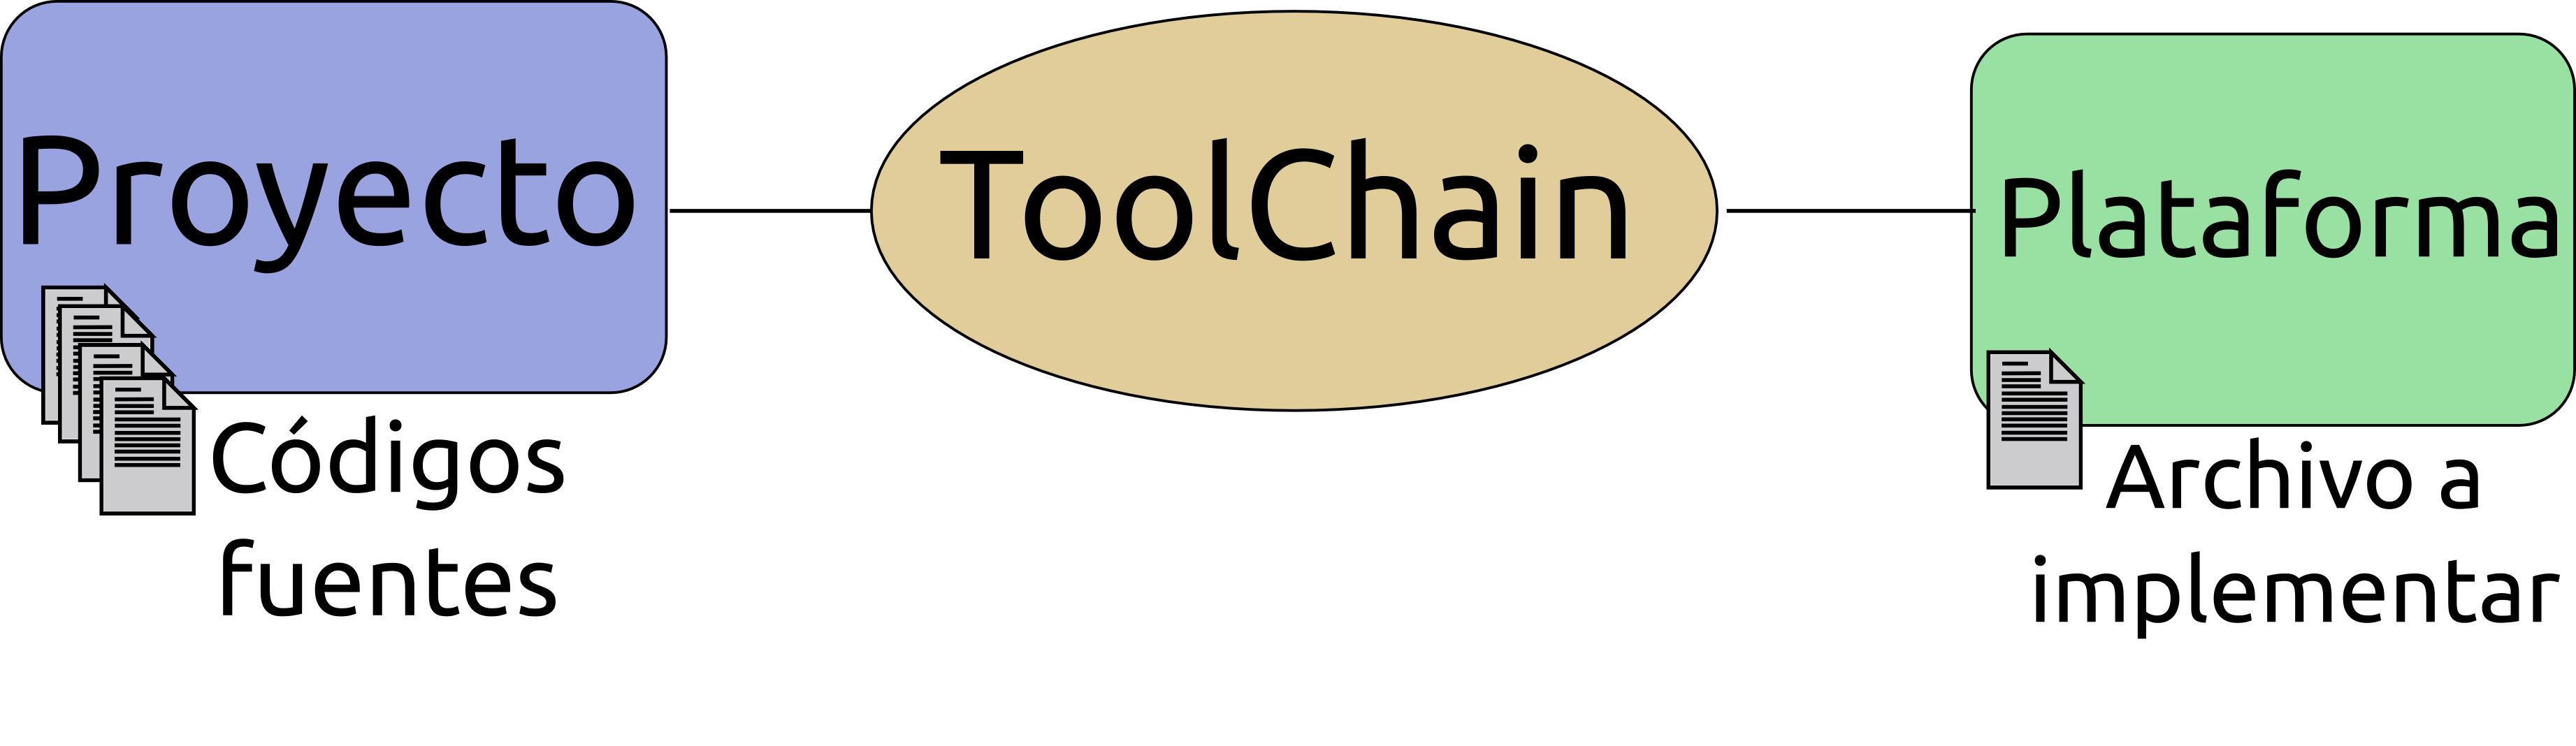
\includegraphics[scale=.5]{./anexo1/images/toolchain_reducido} \end{center}
  \caption{Flujo de dise�o SW utilizando la cadena de herramientas GNU}\label{toolchain_flow}
\end{figure}

\section{Flujo de dise�o software}
%R Real-Time Concepts for Embedded Systems
En la figura \ref{toolchain_flow} se ilustra la secuencia de pasos que se realizan desde la creaci�n de un archivo de texto que posee el c�digo fuente de una aplicaci�n hasta su implementaci�n en la tarjeta de desarrollo. Los pasos necesarios para generar un ejecutable para un sistema embebido son:

\begin{figure}[h]
  \begin{center} 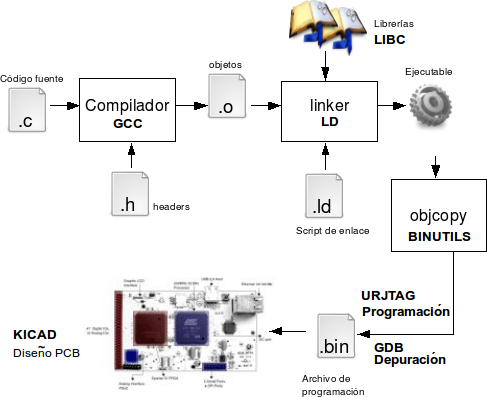
\includegraphics[scale=.6]{./anexo1/images/SW_design_flow} \end{center}
  \caption{Flujo de dise�o SW utilizando la cadena de herramientas GNU}\label{toolchain_flow}
\end{figure}

\begin{enumerate}
 \item \textbf{Escritura del c�digo fuente:} Los entornos de desarrollo \textit{software} IDE (\textit{integrated development environment}) proveen de un editor de texto y la colecci�n de herramientas est�n integradas en la misma aplicaci�n, para el caso de desarrollo de aplicaciones con \textit{software} libre existen alternativas como \url{www.eclipse.com} para la integraci�n de herramientas, pero no es un requisito para escribir c�digos fuentes el uso de un editor en particualar, cada programador puede escribir sus c�digos en la interfaz que le resulte m�s amigable. Los codigos fuentes de los programas para sistemas embebidos generalmente son escritos en C/C++. Algunas partes espec�ficas son escritas en lenguaje ensamblador por motivos de eficiencia en tiempo de ejecuci�n o tama�o. 

 \item \textbf{Compilaci�n:} Los archivos fuentes C y los archivos de ensamblador (generamente s) son tomados por las herramientas de compilaci�n para crear archivos tipo objetos. Estos objetos contienen las instrucciones que el procesador deber� ejecutar cuando las funciones sean invocadas para cumplir con la funcionalidad deseada. Adem�s, estos archivos contienen la informaci�n de las etiquetas usadas en el proceso de enlazado e informaci�n sobre la compilaci�n misma. Por �ltimo, los objetos no contienen las direcciones espec�ficas de donde se implementa una funci�n, por ejemplo, el compilador busca en los encabezados (\textit{headers} .h) de la funci�n \textit{printf} en la librerira \textit{stdio.h}, pero no busca el segmento de c�digo donde est� implementada.
%!!!Aqu� voy JRB-- Adecuando cosas!!!!!!!!!!!!!!!!!!!!!!!!!!!!!!!!!!!!!!!
 \item \textbf{Enlazado:} En esta etapa se realizan dos tareas: 
  \begin{enumerate} 
    \item Se enlazan los archivos tipo objeto del proyecto junto con las librer�as, si una determinada funci�n no es definida por ninguna de las librer�as pasadas como par�metro al enlazador (\textit{linker}), este generar� un error y no se generar� el ejecutable.
    \item Se definen la posiciones f�sicas de las secciones del ejecutable (tipo ELF), esto se realiza a trav�s de un \textit{script de enlazado} que define de forma expl�cita su localizaci�n.
  \end{enumerate}

 \item \textbf{Extracci�n del archivo de programaci�n} En algunas aplicaciones es necesario extraer �nicamente las secciones que residen en los medios de almacenamiento no vol�til y eliminar las dem�s secciones del ejecutable. Esto se realiza con la herramienta \textit{objcopy}, la cual, permite generar archivos en la mayor�a de los formatos soportados por los programadores de memorias y procesadores, como por ejemplo S19 e Intel Hex. Adicionalmente se puede generar un archivo binario que contiene las instrucciones en lenguaje del procesador, y pueden ser descargadas directamente a la memoria de la plataforma.

 \item \textbf{Descarga del programa}. Dependiendo de la plataforma, existen varios m�todos para descargar el archivo de programaci�n:
  \begin{enumerate}
    \item Utilizando un \textit{loader}: El \textit{loader} es una aplicaci�n que reside en un medio de almacenamiento no vol�til y permite la descarga de archivos utilizando el puerto serie o una interfaz de red a una memoria no vol�til externa.
    \item Utilizando el puerto JTAG: El puerto JTAG (Joint Test Action Group) proporciona una interfaz capaz de controlar los registros internos del procesador, y de esta forma, acceder a las memorias de la plataforma y ejecutar un programa residente en una posici�n de memoria determinada.
  \end{enumerate}
%! Recordar que hay una etapa donde se dedica completamente a las interfases de programaci�n
 \item \textbf{Depuraci�n} Una vez se descarga la aplicaci�n a la plataforma es necesario someterla a una serie de pruebas, para verificar su correcto funcionamiento. Esto se puede realizar con el depurador GNU (GDB) y una interfaz de comunicaci�n que puede ser un puerto serie, USB o un adaptador de red.
 
\end{enumerate}

\subsubsection{GNU binutils}
Todas las aplicaciones mencionadas a continuaci�n hacen parte de la cadena de herramientas GNU, que son parte de los recursos suministrados por la comunidad de software libre.
Colecci�n de utilidades para archivos binarios y est�n compuestas por:

\begin{itemize}
 \item  \textbf{addr2line} Convierte direcciones de un programa en nombres de archivos y n�meros de l�nea. Dada una direcci�n y un ejecutable, usa la informaci�n de depuraci�n en el ejecutable para determinar que nombre de archivo y n�mero de l�nea est� asociado con la direcci�n dada.
 \item  \textbf{ar} Esta utilidad crea, modifica y extrae desde ficheros; un fichero es una colecci�n de otros archivos en una estructura que hace posible obtener los archivos individuales. 
 \item  \textbf{as} Utilidad que compila la salida del compilador de C (GCC).
 \item  \textbf{c++filt} Este programa realiza un mapeo inverso: Decodifica nombres de bajo-nivel en nombres a nivel de usuario, de tal forma que el \textit{linker} pueda mantener estas funciones sobrecargadas (overloaded) ``from clashing''. 
 \item  \textbf{gasp} GNU Assembler Macro Preprocessor
 \item  \textbf{ld} El \textit{linker} GNU combina un n�mero de objetos y ficheros, re-localiza sus datos y los relaciona con referencias. Normalmente el �ltimo paso en la construcci�n de un nuevo programa es el llamado a ld.
 \item  \textbf{nm} Realiza un listado de s�mbolos de archivos tipo objeto.
 \item  \textbf{objcopy} Copia los contenidos de un archivo tipo objeto a otro. \textit{objcopy} utiliza la librer�a GNU BFD para leer y escribir el archivo tipo objeto. Permite escribir el archivo destino en un formato diferente al del archivo fuente. 
 \item  \textbf{objdump} Despliega informaci�n sobre archivos tipo objeto. 
 \item  \textbf{ranlib} Genera un �ndice de contenidos de un fichero, y lo almacena en �l.
 \item  \textbf{readelf} Interpreta encabezados de un archivo ELF.
 \item  \textbf{size} Lista el tama�o de las secciones y el tama�o total de un archivo tipo objeto.
 \item  \textbf{strings} Imprime las secuencias de caracteres imprimibles de al menos 4 caracteres de longitud. 
 \item  \textbf{strip} Elimina todos los s�mbolos de un archivo tipo objeto.
\end{itemize}

\subsubsection{Compilador}
El \textit{GNU Compiler Collection} normalmente llamado GCC, es un grupo de compiladores de lenguajes de programaci�n producido por el proyecto GNU. Es el compilador est�ndar para el software libre, de los sistemas operativos basados en Unix y algunos propietarios como Mac OS de Apple. Soporta los lenguajes ADA, C, C++, Fortran, Java, Objective-C, Objective-C++ para las arquitecturas Alpha, ARM, Atmel AVR, Blackfin, H8/300, System/370, System/390, IA-32 (x86), x86-64, IA-64 i.e. the "Itanium", Motorola 68000, Motorola 88000, MIPS, PA-RISC, PDP-11, PowerPC, SuperH, SPARC, VAX, Renesas R8C/M16C/M32C y MorphoSys. Gracias a esto puede considerarse como una herramienta universal para el desarrollo de sistemas embebidos, el c�digo escrito en una plataforma (en un lenguaje de alto nivel) puede ser implementado en otra sin mayores cambios, esto elimina la dependencia entre el c�digo fuente y el procesador (re-utilizaci�n de c�digo), lo que no es posible cuando se utiliza el lenguaje ensamblador. 

\subsubsection{GNU Debugger}
El depurador oficial de GNU (GDB) al igual que GCC, soporta m�ltiples lenguajes y plataformas; permite monitorear y modificar las variables internas del programa y hacer llamado a funciones de forma independiente a la ejecuci�n normal del mismo. Adem�s, permite establecer sesiones remotas utilizando el puerto serie o TCP/IP. Aunque GDB es una aplicaci�n que se ejecuta en consola de comandos, se han desarrollado varios front-ends como DDD o GDB/Insight.

\subsubsection{Librer�as C}
Es necesario contar con las librer�as standard de C: stdio, stdlib, math, etc; las m�s utilizadas en sistemas embebidos son:

\begin{itemize}
 \item \textbf{glibc} Es la librer�a C oficial del proyecto GNU; el principal inconveniente al trabajar con esta librer�a en sistemas embebidos es que genera ejecutables de mayor tama�o que los generados a partir de otras librer�as, lo cual no la hace muy atractiva para este tipo de aplicaciones. 
 \item \textbf{uClibc} Es una librer�a dise�ada especialmente para sistemas embebidos, es mucho m�s peque�a que \textbf{glibc}.
 \item \textbf{newlib} Al igual que \textbf{uClibc}, est� dise�ada para sistemas embebidos. El t�pico ``Hello, world!'' ocupa menos de 30k en un entorno basado en newlib, mientras que en uno basado en glibc, puede ocupar 380k. 
 \item \textbf{diet libc} Es una versi�n de \textit{libc} optimizada en tama�o, puede ser utilizada para crear ejecutables est�ticamente enlazados para Linux en plataformas alpha, arm, hppa, ia64, i386, mips, s390, sparc, sparc64, ppc y x86\_64.
\end{itemize}

\subsection{El formato ELF}

\subsubsection{El formato \textbf{ELF}}

El formato ELF (\textit{Executable and Linkable Format}) Es un est�ndar para objetos, librer�as y ejecutables y es el formato que generan las herramientas GNU. Como puede verse en la figura \ref{elf1} un ejecutable \textit{ELF} est� compuesto por las secciones (\textit{link view}) o segmentos (\textit{execution view}). Si un programador est� interesado en obtener informaci�n de secciones sobre tablas de s�mbolos, c�digo ejecutable espec�fico o informaci�n de enlazado din�mico debe utilizar \textit{link view}. Pero si busca informaci�n sobre segmentos, como por ejemplo, la localizaci�n de los segmentos \textit{text} o \textit{data} debe utilizar \textit{execution view}. El encabezado describe el layout del archivo, proporcionando informaci�n de la forma de acceder a las secciones \cite{MLH98}.
%! Esta imagen me toca cambiarla vectorizarla o hacer una tabla!
\begin{figure}[h]
  \begin{center} \includegraphics[scale=.4]{./anexo1/images/ELF_Link_exec1} \end{center}
  \caption{Formato ELF}\label{elf1}
\end{figure}

Las secciones pueden almacenar c�digo ejecutable, datos, informaci�n de enlazado din�mico, datos de depuraci�n, tablas de s�mbolos,comentarios, tablas de cadenas, y notas. Las secciones m�s importantes son:

\begin{itemize}
 \item \textbf{.bss}            Datos no inicializados. (RAM)
 \item \textbf{.comment}        Informaci�n de la versi�n.
 \item \textbf{.data y .data1}  Datos inicializados.    (RAM)
 \item \textbf{.debug}          Informaci�n para depuraci�n simb�lica. 
 \item \textbf{.dynamic}        Informaci�n sobre enlace din�mico 
 \item \textbf{.dynstr}         Strings necesarios para el enlace din�mico 
 \item \textbf{.dynsym}         Tabla de s�mbolos utilizada para enlace din�mico.
 \item \textbf{.fini}           C�digo de terminaci�n de proceso.
 \item \textbf{.init}           C�digo de inicializaci�n de proceso.
 \item \textbf{.line}           Informaci�n de n�mero de l�nea para depuraci�n simb�lica.
 \item \textbf{.rodata y .rodta1} Datos de solo-lectura (ROM)
 \item \textbf{.shstrtab}       Nombres de secciones.
 \item \textbf{.symtab}         Tabla de s�mbolos.
 \item \textbf{.text}           Instrucciones ejecutables (ROM)
\end{itemize}

%Falta explicar los ELF dinamicos usados en linux y un ejemplo de como la memoria virtual usa estos archivos

%% Ejemplo de aplicaci�n
Para aclarar el contenido de cada una de estas secciones, consideremos la siguiente aplicaci�n sencilla:

\begin{lstlisting}
#include <stdio.h>

int global;
int global_1 = 1;

int main(void)
{
  int i;                                // Variable no inicializada
  int j = 2;                            // Variable inicializada
  for(i=0; i<10; i++){
    printf("Printing %d\n", i*j);       // Caracteres constantes
    j = j + 1;
    global   = i;
    global_1 = i+j;
  }
  return 0;
}
\end{lstlisting}

Generemos el objeto compil�ndolo con el siguiente comando:
\textit{arm-none-linux-gnueabi-gcc -c hello.c}

Examinemos que tipo de secciones tiene este ejecutable
\textit{arm-none-linux-gnueabi-readelf -S hello.o}

\begin{lstlisting}[style=numbered]
Section Headers:
  [Nr] Name              Type            Addr     Off    Size   ES Flg Lk Inf Al
  [ 0]                   NULL            00000000 000000 000000 00      0   0  0
  [ 1] .text             PROGBITS        00000000 000034 00009c 00  AX  0   0  4
  [ 2] .rel.text         REL             00000000 000484 000020 08      9   1  4
  [ 3] .data             PROGBITS        00000000 0000d0 000004 00  WA  0   0  4
  [ 4] .bss              NOBITS          00000000 0000d4 000000 00  WA  0   0  1
  [ 5] .rodata           PROGBITS        00000000 0000d4 000010 00   A  0   0  4
  [ 6] .comment          PROGBITS        00000000 0000e4 00004d 00      0   0  1
  [ 7] .ARM.attributes   ARM_ATTRIBUTES  00000000 000131 00002e 00      0   0  1
  [ 8] .shstrtab         STRTAB          00000000 00015f 000051 00      0   0  1
  [ 9] .symtab           SYMTAB          00000000 000368 0000f0 10     10  11  4
  [10] .strtab           STRTAB          00000000 000458 00002b 00      0   0  1
Key to Flags:
  W (write), A (alloc), X (execute), M (merge), S (strings)
  I (info), L (link order), G (group), x (unknown)
  O (extra OS processing required) o (OS specific), p (processor specific)
\end{lstlisting}

La secci�n \textit{.text}, como se dijo anteriormente contiene las instrucciones ejecutables, por esta raz�n se marca como ejecutable \textit{``X''} en la columna \textit{Flg}. Es posible ver las instrucciones que se ejecutan en esta secci�n ejecutando:

\textit{arm-none-linux-gnueabi-objdump -d -j .text hello.o}

\begin{lstlisting}[style=numbered]
00000000 <main>:
   0:   e92d4800        stmdb   sp!, {fp, lr}
   4:   e28db004        add     fp, sp, #4      ; 0x4
   8:   e24dd008        sub     sp, sp, #8      ; 0x8
   c:   e3a03002        mov     r3, #2  ; 0x2
  10:   e50b3008        str     r3, [fp, #-8]
  14:   e3a03000        mov     r3, #0  ; 0x0
  18:   e50b300c        str     r3, [fp, #-12]
  1c:   ea000013        b       70 <main+0x70>
  20:   e51b200c        ldr     r2, [fp, #-12]
  24:   e51b3008        ldr     r3, [fp, #-8]
  28:   e0030392        mul     r3, r2, r3
  2c:   e59f005c        ldr     r0, [pc, #92]   ; 90 <.text+0x90>
  30:   e1a01003        mov     r1, r3
  34:   ebfffffe        bl      0 <printf>
  38:   e51b3008        ldr     r3, [fp, #-8]
  3c:   e2833001        add     r3, r3, #1      ; 0x1
  40:   e50b3008        str     r3, [fp, #-8]
  44:   e59f2048        ldr     r2, [pc, #72]   ; 94 <.text+0x94>
  48:   e51b300c        ldr     r3, [fp, #-12]
  4c:   e5823000        str     r3, [r2]
  50:   e51b200c        ldr     r2, [fp, #-12]
  54:   e51b3008        ldr     r3, [fp, #-8]
  58:   e0822003        add     r2, r2, r3
  5c:   e59f3034        ldr     r3, [pc, #52]   ; 98 <.text+0x98>
  60:   e5832000        str     r2, [r3]
  64:   e51b300c        ldr     r3, [fp, #-12]
  68:   e2833001        add     r3, r3, #1      ; 0x1
  6c:   e50b300c        str     r3, [fp, #-12]
  70:   e51b300c        ldr     r3, [fp, #-12]
  74:   e3530009        cmp     r3, #9  ; 0x9
  78:   daffffe8        ble     20 <main+0x20>
  7c:   e3a03000        mov     r3, #0  ; 0x0
  80:   e1a00003        mov     r0, r3
  84:   e24bd004        sub     sp, fp, #4      ; 0x4
  88:   e8bd4800        ldmia   sp!, {fp, lr}
  8c:   e12fff1e        bx      lr
\end{lstlisting}

La secci�n \textit{.data} mantiene las variables inicializadas, y contiene:
 
\textit{arm-none-linux-gnueabi-objdump -d -j .data hello.o}
 
\begin{lstlisting}[style=numbered]
00000000 <global_1>:
   0:   01 00 00 00
\end{lstlisting}

Como vemos, la secci�n \textit{.data} contiene �nicamente el valor de inicializaci�n de la variable \textit{global\_1} (1) y no muestra informaci�n acerca de la variable \textit{j}, esto se debe a que la informaci�n est� en el \textit{stack} del proceso. Si observamos el contenido de la secci�n \textit{.text} observamos que esta variable es asignada en tiempo de ejecuci�n, en la l�nea \textit{0c:} se ve la asignaci�n de esta variable:

\begin{lstlisting}[style=numbered]
0c:   e3a03002        mov     r3, #2  ; 0x2 
10:   e50b3008        str     r3, [fp, #-8]
\end{lstlisting}

La secci�n \textit{.bss} mantiene la informaci�n de las variables no inicializadas. En Linux todas las variables no inicializadas, se inicializaran en cero:

\textit{arm-none-linux-gnueabi-objdump -d -j .bss hello}
 
\begin{lstlisting}[style=numbered]
000145c4 <global>:
    145c4:       00000000
\end{lstlisting}
   
La secci�n \textit{.rodata} contiene los datos que no cambian durante la ejecuci�n del programa, es decir, los de solo lectura, si examinamos esta secci�n obtenemos:
 
\textit{hexdump -C hello.o | grep -i 000000d0} (la secci�n \textit{.rodata} comienza en la posici�n de memoria 0xd4)
 
  
\begin{lstlisting}[style=numbered]
000000d0  01 00 00 00 50 72 69 6e  74 69 6e 67 20 25 64 0a  |....Printing %d.|
000000e0  00 00 00 00 00 47 43 43  3a 20 28 43 6f 64 65 53  |.....GCC: (CodeS|
\end{lstlisting}
 
Observamos que en el archivo se almacena la cadena de caracteres \textit{Printing \%d\\n} la cual no se modifica durante la ejecuci�n del programa.
\subsection{Script del enlazador \textit{Linker}}
\subsubsection{Linker Script}
Como vimos anteriormente, el \textit{linker} es el encargado de agrupar todos los archivos objeto \textit{.o}, y las librer�as necesarias para crear el ejecutable, este \textit{linker} permite definir donde ser�n ubicados los diferentes segmentos del archivo ELF, por medio de un archivo de enlace \textit{linker script}. De esta forma podemos ajustar el ejecutable a plataformas con diferentes configuraciones de memoria. Esto brinda un grado mayor de flexibilidad de la cadena de herramientas GNU. Cuando se dispone de un sistema operativo como Linux no es necesario definir este archivo para los ejecutables, ya que el sistema operativo se encarga de guardar las secciones en el lugar indicado; sin embargo, es necesario tenerlo presente ya que como veremos m�s adelante existe un momento en el que el sistema operativo no ha sido cargado en la plataforma y las aplicaciones que se ejecuten deben proporcionar esta informaci�n. A continuaci�n se muestra un ejemplo de este archivo:

\lstset{emph={flash}, emphstyle=\color{red}, emph={[2]ram,base},emphstyle={[2]\color{blue}}}

\begin{lstlisting}
 /* identify the Entry Point  (_vec_reset is defined in file crt.s)  */
ENTRY(_vec_reset)

/* specify the memory areas  */
MEMORY 
{
    flash : ORIGIN = 0,          LENGTH = 256K    /* FLASH EPROM          */
    ram   : ORIGIN = 0x00200000, LENGTH = 64K     /* static RAM area      */
}

/* define a global symbol _stack_end */
_stack_end = 0x20FFFC;

/* now define the output sections  */
SECTIONS
{
  . = 0;            /* set location counter to address zero  */
  .text :           /* collect all sections that should go into FLASH after startup  */
  {
    *(.text)        /* all .text sections (code)  */
    *(.rodata)      /* all .rodata sections (constants, strings, etc.)  */
    *(.rodata*)     /* all .rodata* sections (constants, strings, etc.)  */
    *(.glue_7)      /* all .glue_7 sections  (no idea what these are) */
    *(.glue_7t)     /* all .glue_7t sections (no idea what these are) */
    _etext = .;     /* define a global symbol _etext just after the last code byte */
  } >flash          /* put all the above into FLASH */

  .data :           /* collect all initialized .data sections that go into RAM  */ 
  {
    _data = .;      /* create a global symbol marking the start of the .data section  */
    *(.data)        /* all .data sections  */
    _edata = .;     /* define a global symbol marking the end of the .data section  */
  } >ram AT >flash  /* put all the above into RAM (but load the LMA initializer copy 
                       into FLASH)  */

  .bss :            /* collect all uninitialized .bss sections that go into RAM  */
  {
    _bss_start = .; /* define a global symbol marking the start of the .bss section */
    *(.bss)         /* all .bss sections  */
  } >ram            /* put all the above in RAM (it will be cleared in the startup code*/
  . = ALIGN(4);     /* advance location counter to the next 32-bit boundary */
  _bss_end = . ;    /* define a global symbol marking the end of the .bss section */
}
_end = .;           /* define a global symbol marking the end of application RAM */
\end{lstlisting}

En las primeras l�neas del archivo aparece la declaraci�n de las memorias de la plataforma; en este ejemplo, tenemos una memoria RAM de 64kB que comienza en la posici�n de memoria 0x00200000 y una memoria flash de 256k que comienza en la posici�n 0x0. A continuaci�n se definen las secciones y el lugar donde ser�n almacenadas; en este caso, las secciones \textit{.text} (c�digo ejecutable) y \textit{.rodata} (datos de solo lectura) se almacenan en una memoria no vol�til la flash. Cuando el sistema sea energizado el procesador ejecutar� el c�digo almacenado en su memoria no vol�til. Las secciones \textit{.data} (variables inicializadas) y \textit{.bss} (variables no inicializadas) se almacenar�n en la memoria vol�til RAM, ya que el acceso a las memorias no vol�tiles son m�s lentas y tienen ciclos de lectura/escritura finitos.

En algunos SoCs no se dispone de una memoria no vol�til, por lo que es necesario que la aplicaci�n sea cargada por completo en la RAM. Algunos desarrolladores prefieren almacenar y ejecutar sus aplicaciones en las memorias vol�tiles durante la etapa de desarrollo, debido a que la programaci�n de las memorias no vol�tiles toman mucho m�s tiempo. Obviamente una vez finalizada la etapa de desarrollo las aplicaciones deben ser almacenadas en memorias no vol�tiles.


%%%%%%%%%%%%%%%%%%%%% %%%%%%%%%%% %%%%%%%%%%%%%%%%%%%%%%%%%%%%%%%%%
%
% This section is intended to provide a review on how to use the 
% GNU Toolchain and its parts to buil SW
%
%%%%%%%%%%%%%%%%%%%%%%%% %%%%%%%%%%%%%%% %%%%%%%%%%%%%%%%%%%%%%%%%%
\section{Herramientas libres para simulaci�n dise�o de Hardware por descripci�n de hardware}


\subsubsection{S�ntesis, simulaci�n y verificaci�n digital}

Para la s�ntesis digital a partir de lenguajes de descripci�n de hardware se utilizan las herramientas gratuitas suministradas por los fabricantes de FPGAs, \textit{webpack} de Xilinx y \textit{Quartus} de Altera; debido a que la estructura interna de las FPGAs solo la conocen los fabricantes\footnote{Es posible obtener informaci�n valiosa de sus patentes por ejemplo: http://www.freepatentsonline.com/6301693.pdf, con este tipo de informaci�n varios proyectos buscan generar herramientas abiertas de s�ntesis}, es obligatorio utilizar sus herramientas para obtener el archivo de configuraci�n.

Para la simulaci�n de sistemas digitales que utilizan como entrada de dise�o lenguajes de descripci�n de hardware existen los simuladores \textit{ICARUS} para verilog y \textit{GHDL} para vhdl; los dos pueden ser utilizados para realizar simulaciones funcionales, post s�ntesis o post place \& route (trabajando en conjunto con las herramientas de los fabricantes) y ambos soportan el formato de salida VCD (definido junto con el lenguaje de descripci�n de hardware verilog por el est�ndar IEEE 1364-2001). Adicionalmente, estas herramientas pueden ser utilizadas en los sistemas operativos m�s utilizados.

Como herramienta de simulaci�n se utilizar� \textit{GTKWAVE}, la cual acepta como entrada archivos en formato \textit{VCD} y puede ser ejecutada en MAC, Linux y Windows. \textit{GTKWAVE} realiza un manejo adecuado de la jerarqu�a del sistema bajo an�lisis, permitiendo observar todas las se�ales de los diferentes m�dulos que componen la jerarqu�a superior, lo que es muy �til en este tipo de simulaciones; en la figura \ref{gtkwave} se puede observar una captura de esta herramienta.

  \begin{figure}[htpb]
    \begin{center} 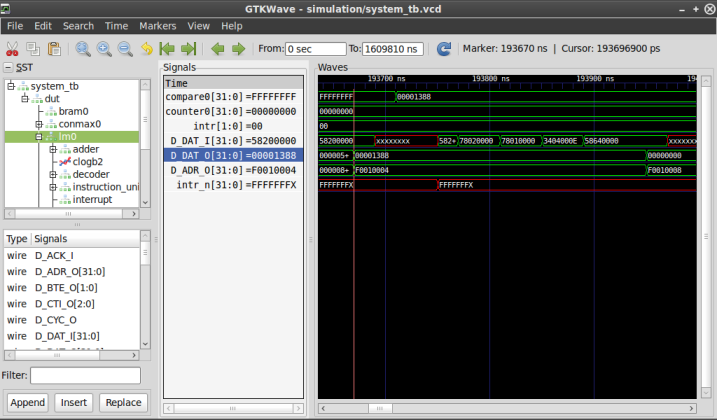
\includegraphics[scale=.7]{./anexo1/images/gtkwave.png}   \end{center}
     \caption{Visualizador de formas de onda \textit{GTKWAVE}} \label{gtkwave}
  \end{figure}

Una vez configurada la FPGA, se utiliza la herramienta \textit{URJTAG} para verificar el correcto funcionamiento del sistema implementado en la FPGA, \textit{URJTAG} proporciona una capa de abstracci�n de hardware que permite el manejo del puerto JTAG de cualquier dispositivo, proporcionando funciones de alto nivel para la aplicaci�n de las funciones JTAG (IDCODE, INTEST, EXTEST, BYPASS, SAMPLE/PRELOAD) permitiendo la aplicaci�n de vectores de prueba al n�cleo l�gico de la FPGA y la captura de la respuesta a estos est�mulos; estas pruebas se realizan a baja frecuencia. \textit{URJTAG} soporta varias interfaces f�sicas para control de las se�ales del puerto JTAG (TDI, TDO, TMS y TCK) las cuales pueden ser conectadas a diferentes puertos de un computador, o como en este caso a un puerto virtual creado en el procesador MIPS.  


\subsubsection{Herramientas para la configuraci�n de PLDs}
Aunque con la plataforma de desarrollo SIE no es necesario utilizar herramientas ni unidades de programaci�n adicionales para configurar su FPGA; el procesador de SIE ejecuta dos aplicaciones que son utilizadas para realizar esta funci�n y pueden ser ejecutadas en computadores personales: \textit{URJTAG} y \textit{XC3SPROG}, las dos funcionan de forma similar, utilizan dispositivos conectados al puerto paralelo (conexi�n directa) o USB (basados en el protocolo MPSSE del chip FT2232) del computador; para ejecutar las instrucciones extendidas de la FPGA CFG\_OUT, CFG\_IN, JSTART y JPROGRAM (hasta el momento solo han sido probadas con las FPGAs de Xilinx).



%%%%%%%%%%%%%%%%%%%%% %%%%%%%%%%% %%%%%%%%%%%%%%%%%%%%%%%%%%%%%%%%%
%
% This section is intended to provide a review on how to use the 
% Programming interfaces
%
%%%%%%%%%%%%%%%%%%%%%%%% %%%%%%%%%%%%%%% %%%%%%%%%%%%%%%%%%%%%%%%%%

\subsection{Interfaz JTAG}
A mediados de los 70s, la estructura de pruebas para tarjetas de circuito impreso (PCB, Printed Circuit Boards) se basaba en el uso de la t�cnica ``bed-of-nails''. Este m�todo utilizaba un dispositivo que conten�a una gran cantidad de puntos de prueba, que permit�an el acceso a dispositivos en la tarjeta a trav�s de puntos colocados en la capa de cobre para dicho fin. Las pruebas se realizaban en dos fases: con el circuito apagado y con el circuito funcionando. Con la aparici�n de los dispositivos de montaje superficial se empez� a colocar dispositivos en las dos caras de la tarjeta, y se redujeron de forma considerable las dimensiones de los dispositivos, disminuyendo la distancia f�sica entre las interconexiones (0.4 - 1mm), dificultando el proceso de pruebas tradicional.

A mediados de los 80s un grupo de ingenieros de pruebas miembros de compa��as electr�nicas europeas se reunieron para examinar el problema y buscar posibles soluciones. Este grupo se auto-denomin� JETAG (Joint European Test Action Group). El m�todo de soluci�n propuesto por ellos estaba basado en el concepto de un registro de corrimiento serial colocado alrededor de la frontera dispositivo, de aqu� el nombre ``Boundary Scan''. Despu�s el grupo se asoci� a compa��as norteamericanas y la ``E'' de ``European'' desapareci� del nombre de la organizaci�n convirti�ndose en JTAG (Join Test Action Group).

\subsubsection{Arquitectura BOUNDARY SCAN} 
A cada se�al de entrada o salida se le adiciona un elemento de memoria multi-prop�sito llamado ``Boundary Scan Cell'' (BSC). Las celdas conectadas a los pines de entrada reciben el nombre de ``Celdas de entrada'', y las que est�n conectadas a los pines de salida ``Celdas de salida''. En la Figura \ref{jtag_basics} se muestra esta arquitectura.

\begin{figure}[h]
  \begin{center} 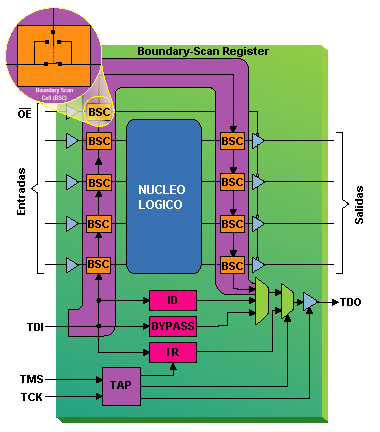
\includegraphics[scale=.6]{./anexo1/images/jtag_basics} \end{center}
  \caption{Arquitectura Boundary Scan} \label{jtag_basics}
\end{figure}

Las BSC se configuran en un registro de corrimiento de entrada y salida paralela. Una carga paralela de los registros (captura) ocasiona que los valores de las se�ales aplicadas a los pines del dispositivo pasen a las celdas de entrada y que opcionalmente los valores de las se�ales internas del dispositivo pasen a las celdas de salida. Una descarga paralela (Actualizaci�n) ocasiona que los valores presentes en las celdas de salida pasen a los pines del dispositivo, y opcionalmente los valores almacenados en las celdas de entrada pasen al interior del dispositivo.

Los datos pueden ser corridos a trav�s del registro de corrimiento de forma serial, empezando por un pin dedicado TDI (Test Data In) y terminando en un pin de salida dedicado llamado TDO (Test Data Out). La se�al de reloj se proporciona por un pin externo TCLK (Test Clock) y el modo de operaci�n se controla por la se�al TMS (Test Mode Select). Los elementos del Boundary Scan no afectan el funcionamiento del dispositivo. Y son independientes del n�cleo l�gico del mismo.

\subsubsection{Instrucciones JTAG}
El Standard IEEE 1149.1 describe tres instrucciones obligatorias: Bypass, Sample/Preload, y Extest \cite{TI96}.

\begin{itemize}
  \item \textbf{BYPASS} Esta instrucci�n permite que el chip permanezca en un modo funcional, hace que el registro de Bypass se coloque entre TDI y TDO; permitiendo la transferencia serial de datos a trav�s del circuito integrado desde TDI hacia TDO sin afectar la operaci�n. La codificaci�n en binario para esta instrucci�n debe ser con todos sus bits en uno. 
  
  \item \textbf{SAMPLE/PRELOAD} Esta instrucci�n selecciona coloca el registro Boundary-Scan entre los terminales TDI y TDO. Durante esta instrucci�n, se puede acceder al registro Boundary-Scan y obtener una muestra de los datos de entrada y salida del chip a trav�s de la operaci�n \textit{Data Scan}. Esta instrucci�n tambi�n se utiliza para precargar los datos de prueba en el registro Boundary-Scan, antes de ejecutar la instrucci�n EXTEST. La codificaci�n de esta instrucci�n la define el fabricante.

  \item \textbf{EXTEST} Esta instrucci�n coloca al circuito integrado en modo de test externo (pruebas de interconexi�n) y conecta el regsitro Boundary-Scan entre TDI y TDO. Las se�ales que salen del circuito son cargadas en el registro boundary-scan en el flanco de bajada de TCK del estado Capture-DR; las se�ales de entrada al dispositivo son cargadas al registro boundary-scan durante el flanco de bajada de TCK dl estado Update-DR (ver Figura \ref{jtag_sm}). La codificaci�n para esta instrucci�n est� definida con todos sus bits en cero.
  
  \item \textbf{INTEST}  La instrucci�n INTEST (opcional) selecciona el registro boundary-scan, pero es utilizado para capturar las se�ales que salen del n�cleo l�gico del dispositivo, y para aplicar valores conocidos a las se�ales de entrada del n�cleo. La codificaci�n para esta se�al es asignada por el dise�ador.
\end{itemize}

\begin{figure}[h]
  \begin{center} 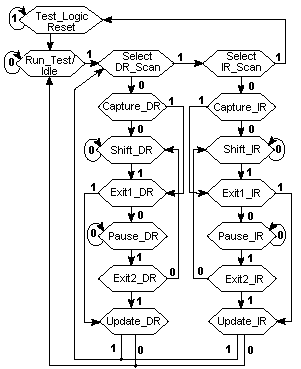
\includegraphics[scale=.8]{./anexo1/images/jtag_sm} \end{center}
  \caption{Arquitectura Boundary Scan} \label{jtag_sm}
\end{figure}



\section{Glosario}
ELF
Objetos
fuentes

binarios
target
reglas
prerequisitos
hdl
codise�o
GNU
GPL
licencias

\section{bib}
No olvidar colocar
Manual del Make tomado de la pagina de GNU project
Managing Projects with GNU Make
		%Herramientas (JRB)

%\bibliography{biblio}

%%%%%%%%%%%%%%%%%%%%%% appendix.tex %%%%%%%%%%%%%%%%%%%%%%%%%%%%%%%%%
%
% sample appendix
%
% Use this file as a template for your own input.
%
%%%%%%%%%%%%%%%%%%%%%%%% Springer-Verlag %%%%%%%%%%%%%%%%%%%%%%%%%%

\appendix
\motto{All's well that ends well}
\chapter{Chapter Heading}
\label{introA} % Always give a unique label
% use \chaptermark{}
% to alter or adjust the chapter heading in the running head

Use the template \emph{appendix.tex} together with the Springer document class SVMono (monograph-type books) or SVMult (edited books) to style appendix of your book in the Springer layout.


\section{Section Heading}
\label{sec:A1}
% Always give a unique label
% and use \ref{<label>} for cross-references
% and \cite{<label>} for bibliographic references
% use \sectionmark{}
% to alter or adjust the section heading in the running head
Instead of simply listing headings of different levels we recommend to let every heading be followed by at least a short passage of text. Furtheron please use the \LaTeX\ automatism for all your cross-references and citations.


\subsection{Subsection Heading}
\label{sec:A2}
Instead of simply listing headings of different levels we recommend to let every heading be followed by at least a short passage of text. Furtheron please use the \LaTeX\ automatism for all your cross-references and citations as has already been described in Sect.~\ref{sec:A1}.

For multiline equations we recommend to use the \verb|eqnarray| environment.
\begin{eqnarray}
\vec{a}\times\vec{b}=\vec{c} \nonumber\\
\vec{a}\times\vec{b}=\vec{c}
\label{eq:A01}
\end{eqnarray}

\subsubsection{Subsubsection Heading}
Instead of simply listing headings of different levels we recommend to let every heading be followed by at least a short passage of text. Furtheron please use the \LaTeX\ automatism for all your cross-references and citations as has already been described in Sect.~\ref{sec:A2}.

Please note that the first line of text that follows a heading is not indented, whereas the first lines of all subsequent paragraphs are.

% For figures use
%
\begin{figure}[t]
\sidecaption[t]
%\centering
% Use the relevant command for your figure-insertion program
% to insert the figure file.
% For example, with the option graphics use
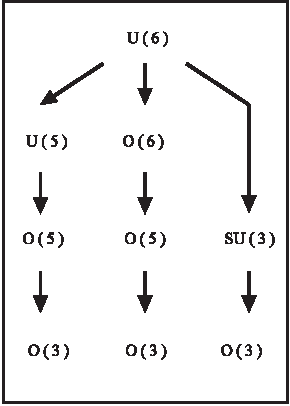
\includegraphics[scale=.65]{figure}
%
% If not, use
%\picplace{5cm}{2cm} % Give the correct figure height and width in cm
%
\caption{Please write your figure caption here}
\label{fig:A1}       % Give a unique label
\end{figure}

% For tables use
%
\begin{table}
\caption{Please write your table caption here}
\label{tab:A1}       % Give a unique label
%
% For LaTeX tables use
%
\begin{tabular}{p{2cm}p{2.4cm}p{2cm}p{4.9cm}}
\hline\noalign{\smallskip}
Classes & Subclass & Length & Action Mechanism  \\
\noalign{\smallskip}\hline\noalign{\smallskip}
Translation & mRNA$^a$  & 22 (19--25) & Translation repression, mRNA cleavage\\
Translation & mRNA cleavage & 21 & mRNA cleavage\\
Translation & mRNA  & 21--22 & mRNA cleavage\\
Translation & mRNA  & 24--26 & Histone and DNA Modification\\
\noalign{\smallskip}\hline\noalign{\smallskip}
\end{tabular}
$^a$ Table foot note (with superscript)
\end{table}
%


%\backmatter%%%%%%%%%%%%%%%%%%%%%%%%%%%%%%%%%%%%%%%%%%%%%%%%%%%%%%%
%%%%%%%%%%%%%%%%%%%%%%%acronym.tex%%%%%%%%%%%%%%%%%%%%%%%%%%%%%%%%%%%%%%%%%
% sample list of acronyms
%
% Use this file as a template for your own input.
%
%%%%%%%%%%%%%%%%%%%%%%%% Springer %%%%%%%%%%%%%%%%%%%%%%%%%%

\Extrachap{Glossary}


Use the template \emph{glossary.tex} together with the Springer document class SVMono (monograph-type books) or SVMult (edited books) to style your glossary\index{glossary} in the Springer layout.


\runinhead{glossary term} Write here the description of the glossary term. Write here the description of the glossary term. Write here the description of the glossary term.

\runinhead{glossary term} Write here the description of the glossary term. Write here the description of the glossary term. Write here the description of the glossary term.

\runinhead{glossary term} Write here the description of the glossary term. Write here the description of the glossary term. Write here the description of the glossary term.

\runinhead{glossary term} Write here the description of the glossary term. Write here the description of the glossary term. Write here the description of the glossary term.

\runinhead{glossary term} Write here the description of the glossary term. Write here the description of the glossary term. Write here the description of the glossary term.
%
\Extrachap{Solutions}

\section*{Problems of Chapter~\ref{intro}}

\begin{sol}{prob1}
The solution\index{problems}\index{solutions} is revealed here.
\end{sol}


\begin{sol}{prob2}
\textbf{Problem Heading}\\
(a) The solution of first part is revealed here.\\
(b) The solution of second part is revealed here.
\end{sol}


%\printindex

%%%%%%%%%%%%%%%%%%%%%%%%%%%%%%%%%%%%%%%%%%%%%%%%%%%%%%%%%%%%%%%%%%%%%%

%\end{document}
%%%%%%%%%%%%%%%%%%%%% chapter.tex %%%%%%%%%%%%%%%%%%%%%%%%%%%%%%%%%
%% At the end, it won't supposed to have
%% %! For Obs
%% %R For bib
%%%%%%%%%%%%%%%%%%%%%%%% Springer-Verlag %%%%%%%%%%%%%%%%%%%%%%%%%% 
%\motto{Use the template \emph{chapter.tex} to style the various elements of your chapter content.}
\chapter{Herramientas libres para construir proyectos Hardware-Software}
\label{intro} % Always give a unique label
%

\begin{svgraybox}
\abstract{En los anteriores cap�tulos se ha tratado el uso de herramientas libres generar tanto los archivos finales a implementar en tanto para dise�os software como para dise�os Hardware. En este cap�tulo se pretende mostrar las diferentes etapas de la construcci�n de los dise�os Hardware/Software a partir de la herramienta Make y la cadena de compilaci�n basada en GCC.}
\end{svgraybox} 

\section{Introduccion}

Introduccion ....

\label{sec:1}

%%%%%%%%%%%%%%%%%%%%% %%%%%%%%%%% %%%%%%%%%%%%%%%%%%%%%%%%%%%%%%%%%
%
% This section is intended to provide a review on how to use the 
% the make to build pojects HW/SW
%
%%%%%%%%%%%%%%%%%%%%%%%% %%%%%%%%%%%%%%% %%%%%%%%%%%%%%%%%%%%%%%%%%
\section{Makefile}
%Para qu� se usa ....
%Implicaciones en el desarrollo de este libro
%El problema que los proyectos son muy extensos en c�digo y reconstruir todo es tedioso y repititivo....
s
El desarrollo de aplicaciones a partir de herramientas libres se apoya en la herramienta de construcci�n \textit{make}, la cual automatiza la creaci�n los archivos binarios de una aplicaci�n. La herramienta construcci�n \textit{make} comunmente llamada constructor, utiliza el archivo \textbf{Makefile} para tomar la especificaci�n del proyecto a construir. Con base en el \textit{Makefile} se ejecutan las reglas necesarias para construir el proyecto. En general el objetivo final del \textit{make} es construir una aplicaci�n, pero dada la flexibilidad que tiene se utiliza para construir cualquier tipo de proyecto que requiera muchas etapas de compilaci�n.

\subsection{Target, prerequisitos y reglas asociadas}

El constructor a trav�s de las reglas descritas en el archivo \textit{Makefile} determina cual y cuando se debe reconstruir un archivo para completar la construcci�n del proyecto completo; todo esto se realiza  en base a las marcas de tiempo de los archivos fuentes y el de salida (\textit{target}). S� los archivos fuentes que son prerequisitos de una regla tiene una marca de tiempo m�s reciente, el constructor determina que este archivo se debe reconstruir.\\

Las reglas del constructor se componen de un \textit{target} o archivo de salida (generalmente un archivo de salida por regla) y una serie de pre-requisitos para cada regla. Los pre-requisitos de cada regla se deben encontrar en las rutas de b�squeda del constructor para completar la construcci�n del proyecto; s� alg�n pre-rerquisito no existe el construcctor buscar� una regla asociada para su construci�n. Dado el caso que no exista alg�n archivo pre-requisito ni una regla asociada a este, el constructor falla con un mensaje de error de falta de pre-requisitos. A continuaci�n se muestra un ejemplo de la sintaxis de una regla para compilar \textit{foo.c} en \textit{foo.o}

\begin{lstlisting}
target1.o:	source1.c header1.h
			gcc -c source1.c
\end{lstlisting}

En las reglas del constructor, el nombre del archivo ubicado antes de los dos puntos (\textbf{:}) se le denomina \textit{target} en este caso \textit{target1.o}\textbf{:}. La lista de archivos que suceden a los dos puntos (\textbf{:}) se le llama la lista de prerequisitos.

Los pre-requisitos son los archivos que el \textit{target} necesita para su construcci�n, en este caso \textit{source1.c} y \textit{header1.h}. El tipo de archivo del \textit{target} y de los prerequisitos no tiene importancia dado que �nicamente se verifica su existenc�a y marca de tiempo. La l�nea que sigue al \textit{target} se le conoce como la primer linea de ejecuci�n de la regla o \textit{recipe}. Es necesario identar con un car�cter de tabulaci�n ($\rightarrow$) las lineas de comandos para que el constructor las ejecute correctamente. La ejecuci�n del \textit{recipe} se realiza en una consola diferente a la en que se invoca el comando \textit{make}. Cuando se tienen lineas muy extensas se puede usar el car�cter \textit{backslash} \textbf{\\}

\subsubsection{Tipos de reglas del constructor}

Existen diferentes tipos de reglas que el constructor puede tomar como referencia para ejecutar comandos externos. Estas reglas pueden ser reglas expl�citas, reglas basadas en comodines, reglas imperativas o reglas vac�as.

\paragraph{Reglas explicitas:} Las reglas expl�citas son las que constructor toma cuando un \textit{target} no se encuentra actualizado. El anterior ejemplo muestra como una regla explicita asociada al \textit{target1.o}. En algunas ocaciones dos o m�s \textit{targets} tienen los mismos prerequisitos para estos casos se pueden definir todos los \textit{targets} en una lista y asociarlos a una sola regla:

\begin{lstlisting}
target1.o target2.o:	source1.c header1.h
\end{lstlisting}

\paragraph{Reglas basadas en comodines \textit{Wildcards}:}

Cuando los proyectos contienen una gran cantidad de objetos por construir la craci�n de un \textit{Makefile} puede tornarse en una tarea repititiva y tomar un tiempo considerable. Para evitar esto el constructor tiene la herramienta de comodines (\textit{wildcards}), los comodines permiten agilizar la creaci�n de un \textit{Makefile} mediante la reducci�n de la cantidad de c�digos que deban construir. Dada la relaci�n estrecha entre el constructor y el \textit{shell} los comodines all� utilizados son heredados por el constructor, los comodines m�s utilizados son:
\begin{itemize}
	\item \textbf{\~}	:   Este s�mbolo se usa para representar la ruta de la carpeta \textit{home} del usuario que ejecuta el constructor.
	\item \textbf{*}	:   El aster�sco es usado para reemplazar una cadena de caracteres completa por ejemplo: Los siguientes archivos \textit{target1.o}, \textit{target2.o} y \textit{target3.o} se pueden representar como \textit{*.o}
	\item \textbf{?}	:   El funcionamiento de este car�cter es similar al \textbf{\*} pero en este caso no se remplaza una cadena completa sino un solo car�cter.
\end{itemize}

\paragraph{Reglas de ejecuci�n imperativa (.\textit{PHONY}):}

Generalmente las reglas incluidas en los \textit{Makefile} son reglas de tipo explicitas, como ya se mencion� estas reglas revisan la relaci�n entre el  \textit{target} y sus prerequisitos. Si se requiere que una regla se ejecute sin tomar en cuenta ninguna relaci�n de los prerequisitos y el \textit{target} se puede usar las reglas de tipo imperativa (.\textit{PHONY}). Un ejemplo claro de cuando se requiere utilizar las reglas imperativas en el caso de tener el siguiente \textit{Makefile}. Este archivo  tiene la regla \textit{clean} la cual no tiene prerequisitos y ejecuta el comando \textbf{rm -f *.o} para eleminar todos los archivos con extensi�n \textit{o}. La ejecuci�n de esta regla se puede realizar mediante  \textbf{\$ make clean}. 

\begin{lstlisting}
clean:
		rm -f *.o
\end{lstlisting}

La anterior regla se ejecuta sin ning�n inconveniente cuando no existe un archivo llamado \textit{clean} dentro de las rutas de b�squeda del cosntructor, dado que no tiene ning�n pre-requisito esta regla siempre se ejecuta al ser invocada. Pero si en la ruta del constructor existe un archivo de nombre \textit{clean} el constructor determina que el \textit{target} de dicha regla se encuentra al d�a y no se debe ejecutar sus comandos de construcci�n terminando su ejecuci�n con la siguiente salida:

\begin{lstlisting}
$ make clean
make: 'clean' is upt to date.
$
\end{lstlisting}

Para prevenir este comportamiento indeseado se puede declarar la regla de la siguiente manera:

\begin{lstlisting}
.PHONY: clean
clean:
		rm -f *.o
\end{lstlisting}

La regla \textit{.PHONY} fuerza la ejecuci�n de esta regla independientemente si el \textit{target} est� al d�a, todos los comandos de la regla se ejecutan cuando es invocada o es pre-requisito de otra regla en ejecuci�n.

Por otra parte existen reglas tipo \textit{PHONY} prestablecidas o est�ndares, estas reglas son definidas directamente por el constructor. Cada una de ellas se muestran en la siguiente tabla:


\begin{table}
\caption{Reglas imperativas comunes}
	\begin{tabular}{p{0.3\textwidth}p{0.7\textwidth}}
	
	\hline
	\textit{Target} & Funci�n (\textit{\$}) \\
	\hline
	
	\textbf{all} 		& 	Realiza todas las tareas necesarias para construir el proyecto \\
	\textbf{install} 	&	Instala la aplicaci�n tomando los binaros compilados \\
	\textbf{clean} 		&	Borra los binarios de la aplicaci�n y los archivos generados en su construcci�n \\
	\textbf{distclean} 	&	Borra todos los archivos generados que no hacen parte del codigo fuente de la distribuci�n \\
	
	
	\end{tabular}
\end{table}

\subsubsection{Reglas vaci�s}

Las reglas vacias son una variante directa de las reglas imperativas; estas reglas generalmente se usan para guardar un evento de construcci�n. La forma en que se puede guardar un evento de construcci�n es mediante la ejecuci�n del comando \textbf{touch} sobre el \textit{target}. 

\begin{lstlisting}
plot: source1.c header1.h
		touch plot
\end{lstlisting}

\subsection{Variables}

Las variables del constructor se utilizan para representar cadenas de caracteres, que pueden hacer referencia a nombres de archivos, directorios, opciones del compilador, programas a ejcutar en la construcci�n de la aplicaci�n, en general puede representar virutalmente cualquier cosa. Para definir una variable se debe ubicar el nombre de la variable en una nueva linea seguido del s�mbolo \textbf{=} y por �ltimo el valor que se desa contener. Para expandir la variable o usar su contenido se usa la misma sintaxis del \textit{bash} \$(\textit{(nombre-variable)})\\

El nombre de una variable no puede contener los carateres especiales \textbf{:}, \textbf{\#}, \textbf{\=} o espacios en blanco, por otra parte los nombres de las variables al igual que la variables del \textit{bash} son sensibles a mayusculas y minusculas. Se recomienda el uso de mayusculas sostenidas para las variables que sean par�metros de conficuraci�n, rutas del sistema y minusculas para el nombre de archivos de salida, programas que se deban ejecutar. 

\subsubsection{Variables autom�ticas}

Las variables autom�ticas permiten acceder a nombres preestablecidos de los componentes de una regla, como el \textit{target}, los prerequisitos. A continuaci�n se listan las variables autom�ticas m�s frecuentes:

\begin{table}
\caption{Variables autom�ticas}
	\begin{tabular}{p{0.1\textwidth}p{0.9\textwidth}}
	\hline
	\textit{Variable} & Funci�n  \\
	\hline

	\textbf{@} 		& Denota el nombre del \textit{target} de la regla.\\
	\textbf{\%}		& Denota el nombre del archivo dentro de una lista.\\
	\textbf{<}		& Es el nombre del primer prerequisito de la regla.\\
	\textbf{?}		& El nombre de todos los prerequisitos de la regla y que tienen una marca de tiempo mayor al \textit{target} en una lista separada poro espacios\\
	\textbf{\^}		& Es la lista de todos los prerequisitos de la regla separada por espacios. Los nombres repetidos son autom�ticamente eliminados para evitar ejecuciones reentrantes en el construcctor.\\
	\textbf{+}		& Es la lista de todos los prerequisitos de la regla separados por espacios, esta lista incluye nombres repetidos. \\
	\textbf{*}		& Es el nombre del archivo de salida sin su extensi�n de salida.
	\end{tabular}
\end{table}

La variables autom�ticas del constructor tambien se deben expandir al llamase es decir, al constructor se le debe decir que el caracter que se est� escribiendo es una variable, para eso se debe anteponer el caracter \textbf{\$} antes de cada variable autom�tica.

%\subsubsection{Variables autom�ticas de rutas de archivos (VPATH y vpath)}

%Cuando se tienen proyectos con gran cantidad de archivos usualmente los desarrolladores crean una estructura de carpetas organizando de esta manera el c�digo.



\section{Makefile}
%Para qu� se usa ....
%Implicaciones en el desarrollo de este libro
%El problema que los proyectos son muy extensos en c�digo y reconstruir todo es tedioso y repititivo....

El desarrollo de aplicaciones con herramientas libres se apoya en la herramienta de construcci�n \textit{make}, la cual automatiza la creaci�n los archivos finales de implementaci�n Hardware/Software. El constructor \textit{make} generalmente utiliza el archivo \textbf{Makefile} como especificaci�n del proyecto que se desee procesar, basado en este el \textit{make} ejecuta las reglas que en �l se especifiquen. En general el objetivo del \textit{make} es construir una aplicaci�n, pero dada la flexibilidad que tiene se utiliza en la construcci�n de casi cualquier tipo de proyecto donde se requieran de muchas etapas en la construcci�n de un proyecto. % No me gusta el final.....JRB

\subsection{Target, prerequisitos y reglas asociadas}

La herramienta \textit{make} a trav�s de las reglas descritas en el archivo \textit{Makefile} determina cual de los objetos o archivos del proyecto debe reconstruir. \textit{make} toma la marca de tiempo del archivo de salida y la de los fuentes, si los fuentes que son prerequisitos de una regla tiene una marca de tiempo mas actual el constructor marca este archivo para su reconstrucci�n. Las reglas del constructor se componen de un \textit{target} (archivo de salida) y una serie de pre-requisitos para cada regla; los pre-requisitos son los archivos que deben existir dentro de las rutas de b�squeda del constructor. A continuaci�n se muestra un ejemplo de un \textit{Makefile} para compilar \textit{foo.c} en \textit{foo.o}

\begin{lstlisting}
target1.o:	source1.c header1.h
			gcc -c source1.c
\end{lstlisting}

El nombre del archivo ubicado antes de los dos puntos (\textbf{:}) se llama \textit{target}, en este caso \textit{target1.o}\textbf{:}, la lista de archivos que suceden a los dos puntos (\textbf{:}) se llama lista de prerequisitos. Los prerequisitos son los archivos necesarios para la construcci�n del \textit{target}, en este caso \textit{source1.c} y \textit{header1.h}. El tipo de archivo del \textit{target} y los prerequisitos no tiene importancia solo su existencia o marca de tiempo. La linea que sigue al \textit{target} se conoce como la primer linea de ejecuci�n de la regla. Las l�neas de de comandos de cosntruci�n sedeben identar con un caracter de tabulaci�n ($\rightarrow$) para que el constructor las ejecute correctamente, esta ejecuci�n se realiza en una consola diferente a la en que se invoca el comando  \textit{make}.

\subsubsection{Tipos de reglas del constructor}

Existen diferentes tipos de reglas que conllevan a la construcci�n de un \textit{target}. Estas reglas pueden ser reglas expl�citas, reglas basadas en comodines, reglas imperativas o reglas vacias.

\paragraph{Reglas explicitas:} Las reglas expl�citas se toman cuando un \textit{target} no se encuentra actualizado. El anterior ejemplo muestra como una regla explicita asociada al \textit{target1.o}. En algunas ocaciones dos o m�s \textit{targets} tienen los mismos prerequisitos para estos casos se pueden definir todos los \textit{targets} en una lista y asociarlos a una sola regla:

\begin{lstlisting}
target1.o target2.o:	source1.c header1.h
\end{lstlisting}

\paragraph{Reglas basadas en comodines \textit{Wildcards}:}

Cuando los proyectos contienen una gran cantidad de objetos por construir la craci�n de un \textit{Makefile} puede tornarse en una tarea repititiva y tomardando un tiempo considerable. Para evitar esto el constructor hereda los comodines (\textit{wildcards}) usados en \textbf{shell}; los comodines permiten agilizar la creaci�n de un \textit{Makefile} mediante la reducci�n de la cantidad c�digo en las reglas de construcci�n, los comodines m�s utilizados son listados acontinuaci�n:
\begin{tabular}{lll}
%\begin{enumerate}[]
	%\item
	
\hline\noalign{\smallskip}
\noalign{\smallskip}\hline\noalign{\smallskip}
	\textbf{\~}	&:&   Este s�mbolo se usa para representar la ruta de la carpeta \textit{home} del usuario que ejecuta el constructor.\\
	%\item
	\textbf{\*}	&:&   El aster�sco es usado para reemplazar una cadena de caracteres completa por ejemplo: Los siguientes archivos \textit{target1.o}, \textit{target2.o} y \textit{target3.o} se pueden representar como \textit{*.o}\\
	%\item
	\textbf{?}	&:&   El funcionamiento de este car�cter es similar al \textbf{\*} pero en este caso no se remplaza una cadena completa sino un solo car�cter.
%\end{enumerate}
\end{tabular}

\paragraph{Reglas de ejecuci�n imperativa (.PHONY):}

Generalmente las reglas incluidas en los \textit{Makefile} son reglas de tipo explicitas, como ya se mencion� estas reglas revisan la relaci�n entre el  \textit{target} y sus prerequisitos. Si se requiere que una regla se ejecute sin tomar en cuenta ninguna relaci�n de los prerequisitos y el \textit{target} se puede usar las reglas de tipo imperativa (.PHONY). Un ejemplo claro de cuando se requiere utilizar las reglas imperativas en el caso de tener el siguiente \textit{Makefile}. Este archivo  tiene la regla \textit{clean} la cual no tiene prerequisitos y ejecuta el comando \textbf{rm -f *.o} para eleminar todos los archivos con extensi�n \textit{o}. La ejecuci�n de esta regla se puede realizar mediante  \textbf{\$ make clean}. 

\begin{lstlisting}
clean:
		rm -f *.o
\end{lstlisting}

La anterior regla se ejecuta sin ning�n inconveniente cuando no existe un archivo llamado \textit{clean} dentro de las rutas de b�squeda del cosntructor, dado que no tiene ning�n pre-requisito esta regla siempre se ejecuta al ser invocada. Pero si en la ruta del constructor existe un archivo de nombre \textit{clean} el constructor determina que el \textit{target} de dicha regla se encuentra al d�a y no se debe ejecutar sus comandos de construcci�n terminando su ejecuci�n con la siguiente salida:

\begin{lstlisting}
\$ make clean
make: 'clean' is upt to date.
\end{lstlisting}

Para prevenir este comportamiento indeseado se puede declarar la regla de la siguiente manera:

\begin{lstlisting}
.PHONY: clean
clean:
		rm -f *.o
\end{lstlisting}

La regla \textit{.PHONY} fuerza la ejecuci�n de la regal clean independientemente si el \textit{target} est� al d�a, todos los comandos de la regla se ejecutan cuando se invoca o es pre-requisito de otra regla en ejecuci�n.

Por otra parte existen reglas tipo \textit{PHONY} prestablecidas o est�ndares, estas reglas son definidas directamente por el constructor. Cada una de ellas se muestran en la siguiente tabla:

\begin{tabular}{llr}
\hline\noalign{\smallskip}
Nombre de regla \textit{target} & Funci�n (\$) \\
\noalign{\smallskip}\hline\noalign{\smallskip}
\textbf{all} 		& 		Realiza todas las tareas necesarias para construir el proyecto \\
\textbf{install}	& 		Instala la aplicaci�n tomando los binaros compilados \\
\textbf{clean}		&		Borra los binarios de la aplicaci�n y los archivos generados en su construcci�n \\
\textbf{distclean}	&		Borra todos los archivos generados que no hacen parte del codigo fuente de la
%\noalign{\smallskip}
\end{tabular}


\subsubsection{Reglas vacias}
=======
%%%%%%%%%%%%%%%%%%%%% %%%%%%%%%%% %%%%%%%%%%%%%%%%%%%%%%%%%%%%%%%%%
%
% This section is intended to provide a review on how to use the 
% GNU Toolchain and its parts to buil SW
%
%%%%%%%%%%%%%%%%%%%%%%%% %%%%%%%%%%%%%%% %%%%%%%%%%%%%%%%%%%%%%%%%%

\section{Herramientas compilaci�n y desarrollo de proyectos SW}%%%Esto est� feo.... Nombre m�s espec�fico

%!Esto necesita sustento en un libro falta incluir referencias de esta secci�n

%!Esto es solo una idea de introducci�n a la secci�n falta cambiar
Para el desarrollo de aplicaciones \textit{software} mediante lenguales de alto nivel perm�ten acelerar el desarrollo de la aplicaci�n, pero requiere de un conjunto de herramientas para la creaci�n del archivo final. Estas herramientas llevan el conjunto de archivos fuentes y paso a paso los convierten en un archivo ejecutable por la m�quina, llamado binario. 

%!Esta figura toca hacerla conteniendo las dos y explicarlas en el texto de abajo
\begin{figure}[h]
  \begin{center} 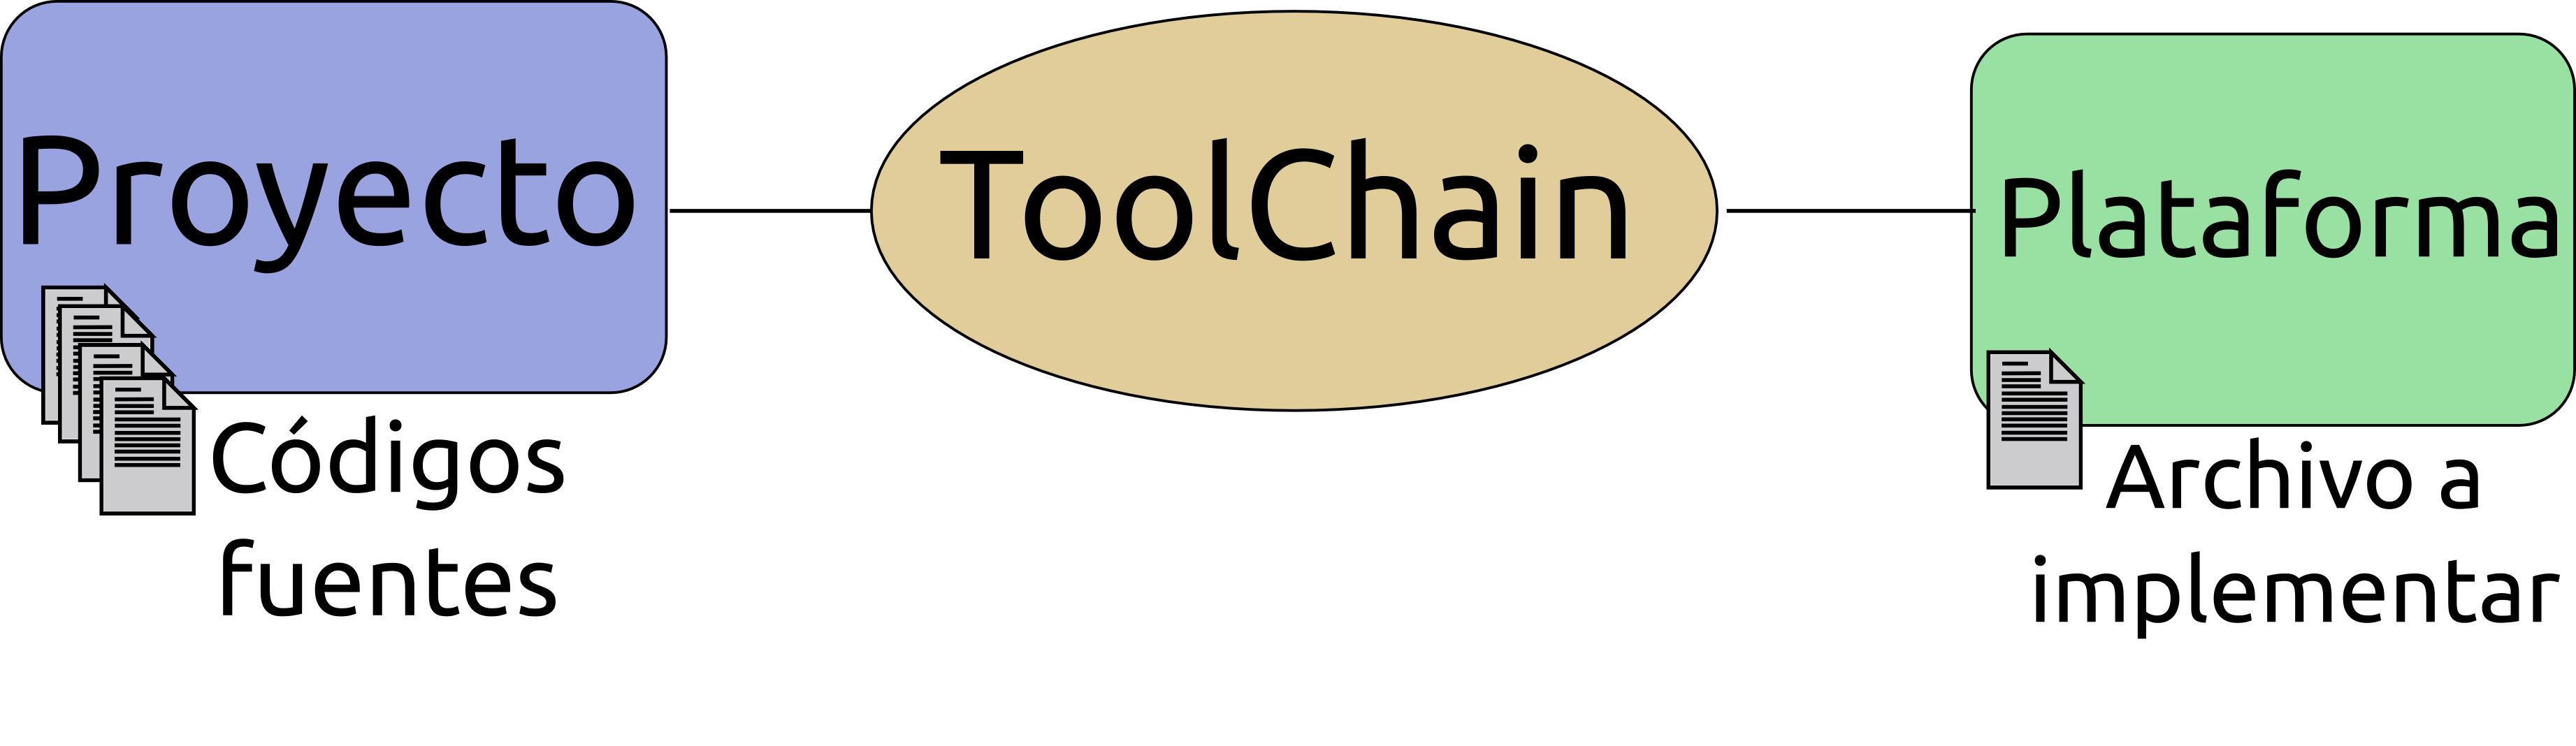
\includegraphics[scale=.5]{./anexo1/images/toolchain_reducido} \end{center}
  \caption{Flujo de dise�o SW utilizando la cadena de herramientas GNU}\label{toolchain_flow}
\end{figure}

\section{Flujo de dise�o software}
%R Real-Time Concepts for Embedded Systems
En la figura \ref{toolchain_flow} se ilustra la secuencia de pasos que se realizan desde la creaci�n de un archivo de texto que posee el c�digo fuente de una aplicaci�n hasta su implementaci�n en la tarjeta de desarrollo. Los pasos necesarios para generar un ejecutable para un sistema embebido son:

\begin{figure}[h]
  \begin{center} 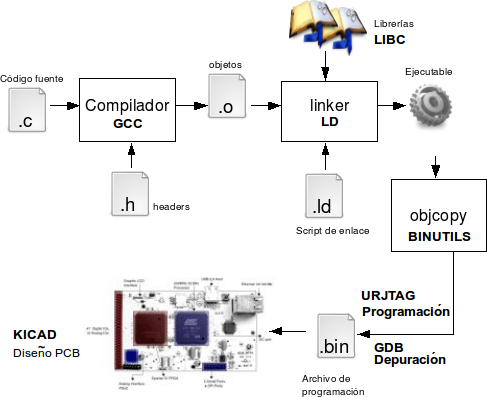
\includegraphics[scale=.6]{./anexo1/images/SW_design_flow} \end{center}
  \caption{Flujo de dise�o SW utilizando la cadena de herramientas GNU}\label{toolchain_flow}
\end{figure}

\begin{enumerate}
 \item \textbf{Escritura del c�digo fuente:} Los entornos de desarrollo \textit{software} IDE (\textit{integrated development environment}) proveen de un editor de texto y la colecci�n de herramientas est�n integradas en la misma aplicaci�n, para el caso de desarrollo de aplicaciones con \textit{software} libre existen alternativas como \url{www.eclipse.com} para la integraci�n de herramientas, pero no es un requisito para escribir c�digos fuentes el uso de un editor en particualar, cada programador puede escribir sus c�digos en la interfaz que le resulte m�s amigable. Los codigos fuentes de los programas para sistemas embebidos generalmente son escritos en C/C++. Algunas partes espec�ficas son escritas en lenguaje ensamblador por motivos de eficiencia en tiempo de ejecuci�n o tama�o. 

 \item \textbf{Compilaci�n:} Los archivos fuentes C y los archivos de ensamblador (generamente s) son tomados por las herramientas de compilaci�n para crear archivos tipo objetos. Estos objetos contienen las instrucciones que el procesador deber� ejecutar cuando las funciones sean invocadas para cumplir con la funcionalidad deseada. Adem�s, estos archivos contienen la informaci�n de las etiquetas usadas en el proceso de enlazado e informaci�n sobre la compilaci�n misma. Por �ltimo, los objetos no contienen las direcciones espec�ficas de donde se implementa una funci�n, por ejemplo, el compilador busca en los encabezados (\textit{headers} .h) de la funci�n \textit{printf} en la librerira \textit{stdio.h}, pero no busca el segmento de c�digo donde est� implementada.
%!!!Aqu� voy JRB-- Adecuando cosas!!!!!!!!!!!!!!!!!!!!!!!!!!!!!!!!!!!!!!!
 \item \textbf{Enlazado:} En esta etapa se realizan dos tareas: 
  \begin{enumerate} 
    \item Se enlazan los archivos tipo objeto del proyecto junto con las librer�as, si una determinada funci�n no es definida por ninguna de las librer�as pasadas como par�metro al enlazador (\textit{linker}), este generar� un error y no se generar� el ejecutable.
    \item Se definen la posiciones f�sicas de las secciones del ejecutable (tipo ELF), esto se realiza a trav�s de un \textit{script de enlazado} que define de forma expl�cita su localizaci�n.
  \end{enumerate}

 \item \textbf{Extracci�n del archivo de programaci�n} En algunas aplicaciones es necesario extraer �nicamente las secciones que residen en los medios de almacenamiento no vol�til y eliminar las dem�s secciones del ejecutable. Esto se realiza con la herramienta \textit{objcopy}, la cual, permite generar archivos en la mayor�a de los formatos soportados por los programadores de memorias y procesadores, como por ejemplo S19 e Intel Hex. Adicionalmente se puede generar un archivo binario que contiene las instrucciones en lenguaje del procesador, y pueden ser descargadas directamente a la memoria de la plataforma.

 \item \textbf{Descarga del programa}. Dependiendo de la plataforma, existen varios m�todos para descargar el archivo de programaci�n:
  \begin{enumerate}
    \item Utilizando un \textit{loader}: El \textit{loader} es una aplicaci�n que reside en un medio de almacenamiento no vol�til y permite la descarga de archivos utilizando el puerto serie o una interfaz de red a una memoria no vol�til externa.
    \item Utilizando el puerto JTAG: El puerto JTAG (Joint Test Action Group) proporciona una interfaz capaz de controlar los registros internos del procesador, y de esta forma, acceder a las memorias de la plataforma y ejecutar un programa residente en una posici�n de memoria determinada.
  \end{enumerate}
%! Recordar que hay una etapa donde se dedica completamente a las interfases de programaci�n
 \item \textbf{Depuraci�n} Una vez se descarga la aplicaci�n a la plataforma es necesario someterla a una serie de pruebas, para verificar su correcto funcionamiento. Esto se puede realizar con el depurador GNU (GDB) y una interfaz de comunicaci�n que puede ser un puerto serie, USB o un adaptador de red.
 
\end{enumerate}

\subsubsection{GNU binutils}
Todas las aplicaciones mencionadas a continuaci�n hacen parte de la cadena de herramientas GNU, que son parte de los recursos suministrados por la comunidad de software libre.
Colecci�n de utilidades para archivos binarios y est�n compuestas por:

\begin{itemize}
 \item  \textbf{addr2line} Convierte direcciones de un programa en nombres de archivos y n�meros de l�nea. Dada una direcci�n y un ejecutable, usa la informaci�n de depuraci�n en el ejecutable para determinar que nombre de archivo y n�mero de l�nea est� asociado con la direcci�n dada.
 \item  \textbf{ar} Esta utilidad crea, modifica y extrae desde ficheros; un fichero es una colecci�n de otros archivos en una estructura que hace posible obtener los archivos individuales. 
 \item  \textbf{as} Utilidad que compila la salida del compilador de C (GCC).
 \item  \textbf{c++filt} Este programa realiza un mapeo inverso: Decodifica nombres de bajo-nivel en nombres a nivel de usuario, de tal forma que el \textit{linker} pueda mantener estas funciones sobrecargadas (overloaded) ``from clashing''. 
 \item  \textbf{gasp} GNU Assembler Macro Preprocessor
 \item  \textbf{ld} El \textit{linker} GNU combina un n�mero de objetos y ficheros, re-localiza sus datos y los relaciona con referencias. Normalmente el �ltimo paso en la construcci�n de un nuevo programa es el llamado a ld.
 \item  \textbf{nm} Realiza un listado de s�mbolos de archivos tipo objeto.
 \item  \textbf{objcopy} Copia los contenidos de un archivo tipo objeto a otro. \textit{objcopy} utiliza la librer�a GNU BFD para leer y escribir el archivo tipo objeto. Permite escribir el archivo destino en un formato diferente al del archivo fuente. 
 \item  \textbf{objdump} Despliega informaci�n sobre archivos tipo objeto. 
 \item  \textbf{ranlib} Genera un �ndice de contenidos de un fichero, y lo almacena en �l.
 \item  \textbf{readelf} Interpreta encabezados de un archivo ELF.
 \item  \textbf{size} Lista el tama�o de las secciones y el tama�o total de un archivo tipo objeto.
 \item  \textbf{strings} Imprime las secuencias de caracteres imprimibles de al menos 4 caracteres de longitud. 
 \item  \textbf{strip} Elimina todos los s�mbolos de un archivo tipo objeto.
\end{itemize}

\subsubsection{Compilador}
El \textit{GNU Compiler Collection} normalmente llamado GCC, es un grupo de compiladores de lenguajes de programaci�n producido por el proyecto GNU. Es el compilador est�ndar para el software libre, de los sistemas operativos basados en Unix y algunos propietarios como Mac OS de Apple. Soporta los lenguajes ADA, C, C++, Fortran, Java, Objective-C, Objective-C++ para las arquitecturas Alpha, ARM, Atmel AVR, Blackfin, H8/300, System/370, System/390, IA-32 (x86), x86-64, IA-64 i.e. the "Itanium", Motorola 68000, Motorola 88000, MIPS, PA-RISC, PDP-11, PowerPC, SuperH, SPARC, VAX, Renesas R8C/M16C/M32C y MorphoSys. Gracias a esto puede considerarse como una herramienta universal para el desarrollo de sistemas embebidos, el c�digo escrito en una plataforma (en un lenguaje de alto nivel) puede ser implementado en otra sin mayores cambios, esto elimina la dependencia entre el c�digo fuente y el procesador (re-utilizaci�n de c�digo), lo que no es posible cuando se utiliza el lenguaje ensamblador. 

\subsubsection{GNU Debugger}
El depurador oficial de GNU (GDB) al igual que GCC, soporta m�ltiples lenguajes y plataformas; permite monitorear y modificar las variables internas del programa y hacer llamado a funciones de forma independiente a la ejecuci�n normal del mismo. Adem�s, permite establecer sesiones remotas utilizando el puerto serie o TCP/IP. Aunque GDB es una aplicaci�n que se ejecuta en consola de comandos, se han desarrollado varios front-ends como DDD o GDB/Insight.

\subsubsection{Librer�as C}
Es necesario contar con las librer�as standard de C: stdio, stdlib, math, etc; las m�s utilizadas en sistemas embebidos son:

\begin{itemize}
 \item \textbf{glibc} Es la librer�a C oficial del proyecto GNU; el principal inconveniente al trabajar con esta librer�a en sistemas embebidos es que genera ejecutables de mayor tama�o que los generados a partir de otras librer�as, lo cual no la hace muy atractiva para este tipo de aplicaciones. 
 \item \textbf{uClibc} Es una librer�a dise�ada especialmente para sistemas embebidos, es mucho m�s peque�a que \textbf{glibc}.
 \item \textbf{newlib} Al igual que \textbf{uClibc}, est� dise�ada para sistemas embebidos. El t�pico ``Hello, world!'' ocupa menos de 30k en un entorno basado en newlib, mientras que en uno basado en glibc, puede ocupar 380k. 
 \item \textbf{diet libc} Es una versi�n de \textit{libc} optimizada en tama�o, puede ser utilizada para crear ejecutables est�ticamente enlazados para Linux en plataformas alpha, arm, hppa, ia64, i386, mips, s390, sparc, sparc64, ppc y x86\_64.
\end{itemize}

\subsection{El formato ELF}

\subsubsection{El formato \textbf{ELF}}

El formato ELF (\textit{Executable and Linkable Format}) Es un est�ndar para objetos, librer�as y ejecutables y es el formato que generan las herramientas GNU. Como puede verse en la figura \ref{elf1} un ejecutable \textit{ELF} est� compuesto por las secciones (\textit{link view}) o segmentos (\textit{execution view}). Si un programador est� interesado en obtener informaci�n de secciones sobre tablas de s�mbolos, c�digo ejecutable espec�fico o informaci�n de enlazado din�mico debe utilizar \textit{link view}. Pero si busca informaci�n sobre segmentos, como por ejemplo, la localizaci�n de los segmentos \textit{text} o \textit{data} debe utilizar \textit{execution view}. El encabezado describe el layout del archivo, proporcionando informaci�n de la forma de acceder a las secciones \cite{MLH98}.
%! Esta imagen me toca cambiarla vectorizarla o hacer una tabla!
\begin{figure}[h]
  \begin{center} \includegraphics[scale=.4]{./anexo1/images/ELF_Link_exec1} \end{center}
  \caption{Formato ELF}\label{elf1}
\end{figure}

Las secciones pueden almacenar c�digo ejecutable, datos, informaci�n de enlazado din�mico, datos de depuraci�n, tablas de s�mbolos,comentarios, tablas de cadenas, y notas. Las secciones m�s importantes son:

\begin{itemize}
 \item \textbf{.bss}            Datos no inicializados. (RAM)
 \item \textbf{.comment}        Informaci�n de la versi�n.
 \item \textbf{.data y .data1}  Datos inicializados.    (RAM)
 \item \textbf{.debug}          Informaci�n para depuraci�n simb�lica. 
 \item \textbf{.dynamic}        Informaci�n sobre enlace din�mico 
 \item \textbf{.dynstr}         Strings necesarios para el enlace din�mico 
 \item \textbf{.dynsym}         Tabla de s�mbolos utilizada para enlace din�mico.
 \item \textbf{.fini}           C�digo de terminaci�n de proceso.
 \item \textbf{.init}           C�digo de inicializaci�n de proceso.
 \item \textbf{.line}           Informaci�n de n�mero de l�nea para depuraci�n simb�lica.
 \item \textbf{.rodata y .rodta1} Datos de solo-lectura (ROM)
 \item \textbf{.shstrtab}       Nombres de secciones.
 \item \textbf{.symtab}         Tabla de s�mbolos.
 \item \textbf{.text}           Instrucciones ejecutables (ROM)
\end{itemize}

%Falta explicar los ELF dinamicos usados en linux y un ejemplo de como la memoria virtual usa estos archivos

%% Ejemplo de aplicaci�n
Para aclarar el contenido de cada una de estas secciones, consideremos la siguiente aplicaci�n sencilla:

\begin{lstlisting}
#include <stdio.h>

int global;
int global_1 = 1;

int main(void)
{
  int i;                                // Variable no inicializada
  int j = 2;                            // Variable inicializada
  for(i=0; i<10; i++){
    printf("Printing %d\n", i*j);       // Caracteres constantes
    j = j + 1;
    global   = i;
    global_1 = i+j;
  }
  return 0;
}
\end{lstlisting}

Generemos el objeto compil�ndolo con el siguiente comando:
\textit{arm-none-linux-gnueabi-gcc -c hello.c}

Examinemos que tipo de secciones tiene este ejecutable
\textit{arm-none-linux-gnueabi-readelf -S hello.o}

\begin{lstlisting}[style=numbered]
Section Headers:
  [Nr] Name              Type            Addr     Off    Size   ES Flg Lk Inf Al
  [ 0]                   NULL            00000000 000000 000000 00      0   0  0
  [ 1] .text             PROGBITS        00000000 000034 00009c 00  AX  0   0  4
  [ 2] .rel.text         REL             00000000 000484 000020 08      9   1  4
  [ 3] .data             PROGBITS        00000000 0000d0 000004 00  WA  0   0  4
  [ 4] .bss              NOBITS          00000000 0000d4 000000 00  WA  0   0  1
  [ 5] .rodata           PROGBITS        00000000 0000d4 000010 00   A  0   0  4
  [ 6] .comment          PROGBITS        00000000 0000e4 00004d 00      0   0  1
  [ 7] .ARM.attributes   ARM_ATTRIBUTES  00000000 000131 00002e 00      0   0  1
  [ 8] .shstrtab         STRTAB          00000000 00015f 000051 00      0   0  1
  [ 9] .symtab           SYMTAB          00000000 000368 0000f0 10     10  11  4
  [10] .strtab           STRTAB          00000000 000458 00002b 00      0   0  1
Key to Flags:
  W (write), A (alloc), X (execute), M (merge), S (strings)
  I (info), L (link order), G (group), x (unknown)
  O (extra OS processing required) o (OS specific), p (processor specific)
\end{lstlisting}

La secci�n \textit{.text}, como se dijo anteriormente contiene las instrucciones ejecutables, por esta raz�n se marca como ejecutable \textit{``X''} en la columna \textit{Flg}. Es posible ver las instrucciones que se ejecutan en esta secci�n ejecutando:

\textit{arm-none-linux-gnueabi-objdump -d -j .text hello.o}

\begin{lstlisting}[style=numbered]
00000000 <main>:
   0:   e92d4800        stmdb   sp!, {fp, lr}
   4:   e28db004        add     fp, sp, #4      ; 0x4
   8:   e24dd008        sub     sp, sp, #8      ; 0x8
   c:   e3a03002        mov     r3, #2  ; 0x2
  10:   e50b3008        str     r3, [fp, #-8]
  14:   e3a03000        mov     r3, #0  ; 0x0
  18:   e50b300c        str     r3, [fp, #-12]
  1c:   ea000013        b       70 <main+0x70>
  20:   e51b200c        ldr     r2, [fp, #-12]
  24:   e51b3008        ldr     r3, [fp, #-8]
  28:   e0030392        mul     r3, r2, r3
  2c:   e59f005c        ldr     r0, [pc, #92]   ; 90 <.text+0x90>
  30:   e1a01003        mov     r1, r3
  34:   ebfffffe        bl      0 <printf>
  38:   e51b3008        ldr     r3, [fp, #-8]
  3c:   e2833001        add     r3, r3, #1      ; 0x1
  40:   e50b3008        str     r3, [fp, #-8]
  44:   e59f2048        ldr     r2, [pc, #72]   ; 94 <.text+0x94>
  48:   e51b300c        ldr     r3, [fp, #-12]
  4c:   e5823000        str     r3, [r2]
  50:   e51b200c        ldr     r2, [fp, #-12]
  54:   e51b3008        ldr     r3, [fp, #-8]
  58:   e0822003        add     r2, r2, r3
  5c:   e59f3034        ldr     r3, [pc, #52]   ; 98 <.text+0x98>
  60:   e5832000        str     r2, [r3]
  64:   e51b300c        ldr     r3, [fp, #-12]
  68:   e2833001        add     r3, r3, #1      ; 0x1
  6c:   e50b300c        str     r3, [fp, #-12]
  70:   e51b300c        ldr     r3, [fp, #-12]
  74:   e3530009        cmp     r3, #9  ; 0x9
  78:   daffffe8        ble     20 <main+0x20>
  7c:   e3a03000        mov     r3, #0  ; 0x0
  80:   e1a00003        mov     r0, r3
  84:   e24bd004        sub     sp, fp, #4      ; 0x4
  88:   e8bd4800        ldmia   sp!, {fp, lr}
  8c:   e12fff1e        bx      lr
\end{lstlisting}

La secci�n \textit{.data} mantiene las variables inicializadas, y contiene:
 
\textit{arm-none-linux-gnueabi-objdump -d -j .data hello.o}
 
\begin{lstlisting}[style=numbered]
00000000 <global_1>:
   0:   01 00 00 00
\end{lstlisting}

Como vemos, la secci�n \textit{.data} contiene �nicamente el valor de inicializaci�n de la variable \textit{global\_1} (1) y no muestra informaci�n acerca de la variable \textit{j}, esto se debe a que la informaci�n est� en el \textit{stack} del proceso. Si observamos el contenido de la secci�n \textit{.text} observamos que esta variable es asignada en tiempo de ejecuci�n, en la l�nea \textit{0c:} se ve la asignaci�n de esta variable:

\begin{lstlisting}[style=numbered]
0c:   e3a03002        mov     r3, #2  ; 0x2 
10:   e50b3008        str     r3, [fp, #-8]
\end{lstlisting}

La secci�n \textit{.bss} mantiene la informaci�n de las variables no inicializadas. En Linux todas las variables no inicializadas, se inicializaran en cero:

\textit{arm-none-linux-gnueabi-objdump -d -j .bss hello}
 
\begin{lstlisting}[style=numbered]
000145c4 <global>:
    145c4:       00000000
\end{lstlisting}
   
La secci�n \textit{.rodata} contiene los datos que no cambian durante la ejecuci�n del programa, es decir, los de solo lectura, si examinamos esta secci�n obtenemos:
 
\textit{hexdump -C hello.o | grep -i 000000d0} (la secci�n \textit{.rodata} comienza en la posici�n de memoria 0xd4)
 
  
\begin{lstlisting}[style=numbered]
000000d0  01 00 00 00 50 72 69 6e  74 69 6e 67 20 25 64 0a  |....Printing %d.|
000000e0  00 00 00 00 00 47 43 43  3a 20 28 43 6f 64 65 53  |.....GCC: (CodeS|
\end{lstlisting}
 
Observamos que en el archivo se almacena la cadena de caracteres \textit{Printing \%d\\n} la cual no se modifica durante la ejecuci�n del programa.
\subsection{Script del enlazador \textit{Linker}}
\subsubsection{Linker Script}
Como vimos anteriormente, el \textit{linker} es el encargado de agrupar todos los archivos objeto \textit{.o}, y las librer�as necesarias para crear el ejecutable, este \textit{linker} permite definir donde ser�n ubicados los diferentes segmentos del archivo ELF, por medio de un archivo de enlace \textit{linker script}. De esta forma podemos ajustar el ejecutable a plataformas con diferentes configuraciones de memoria. Esto brinda un grado mayor de flexibilidad de la cadena de herramientas GNU. Cuando se dispone de un sistema operativo como Linux no es necesario definir este archivo para los ejecutables, ya que el sistema operativo se encarga de guardar las secciones en el lugar indicado; sin embargo, es necesario tenerlo presente ya que como veremos m�s adelante existe un momento en el que el sistema operativo no ha sido cargado en la plataforma y las aplicaciones que se ejecuten deben proporcionar esta informaci�n. A continuaci�n se muestra un ejemplo de este archivo:

\lstset{emph={flash}, emphstyle=\color{red}, emph={[2]ram,base},emphstyle={[2]\color{blue}}}

\begin{lstlisting}
 /* identify the Entry Point  (_vec_reset is defined in file crt.s)  */
ENTRY(_vec_reset)

/* specify the memory areas  */
MEMORY 
{
    flash : ORIGIN = 0,          LENGTH = 256K    /* FLASH EPROM          */
    ram   : ORIGIN = 0x00200000, LENGTH = 64K     /* static RAM area      */
}

/* define a global symbol _stack_end */
_stack_end = 0x20FFFC;

/* now define the output sections  */
SECTIONS
{
  . = 0;            /* set location counter to address zero  */
  .text :           /* collect all sections that should go into FLASH after startup  */
  {
    *(.text)        /* all .text sections (code)  */
    *(.rodata)      /* all .rodata sections (constants, strings, etc.)  */
    *(.rodata*)     /* all .rodata* sections (constants, strings, etc.)  */
    *(.glue_7)      /* all .glue_7 sections  (no idea what these are) */
    *(.glue_7t)     /* all .glue_7t sections (no idea what these are) */
    _etext = .;     /* define a global symbol _etext just after the last code byte */
  } >flash          /* put all the above into FLASH */

  .data :           /* collect all initialized .data sections that go into RAM  */ 
  {
    _data = .;      /* create a global symbol marking the start of the .data section  */
    *(.data)        /* all .data sections  */
    _edata = .;     /* define a global symbol marking the end of the .data section  */
  } >ram AT >flash  /* put all the above into RAM (but load the LMA initializer copy 
                       into FLASH)  */

  .bss :            /* collect all uninitialized .bss sections that go into RAM  */
  {
    _bss_start = .; /* define a global symbol marking the start of the .bss section */
    *(.bss)         /* all .bss sections  */
  } >ram            /* put all the above in RAM (it will be cleared in the startup code*/
  . = ALIGN(4);     /* advance location counter to the next 32-bit boundary */
  _bss_end = . ;    /* define a global symbol marking the end of the .bss section */
}
_end = .;           /* define a global symbol marking the end of application RAM */
\end{lstlisting}

En las primeras l�neas del archivo aparece la declaraci�n de las memorias de la plataforma; en este ejemplo, tenemos una memoria RAM de 64kB que comienza en la posici�n de memoria 0x00200000 y una memoria flash de 256k que comienza en la posici�n 0x0. A continuaci�n se definen las secciones y el lugar donde ser�n almacenadas; en este caso, las secciones \textit{.text} (c�digo ejecutable) y \textit{.rodata} (datos de solo lectura) se almacenan en una memoria no vol�til la flash. Cuando el sistema sea energizado el procesador ejecutar� el c�digo almacenado en su memoria no vol�til. Las secciones \textit{.data} (variables inicializadas) y \textit{.bss} (variables no inicializadas) se almacenar�n en la memoria vol�til RAM, ya que el acceso a las memorias no vol�tiles son m�s lentas y tienen ciclos de lectura/escritura finitos.

En algunos SoCs no se dispone de una memoria no vol�til, por lo que es necesario que la aplicaci�n sea cargada por completo en la RAM. Algunos desarrolladores prefieren almacenar y ejecutar sus aplicaciones en las memorias vol�tiles durante la etapa de desarrollo, debido a que la programaci�n de las memorias no vol�tiles toman mucho m�s tiempo. Obviamente una vez finalizada la etapa de desarrollo las aplicaciones deben ser almacenadas en memorias no vol�tiles.


%%%%%%%%%%%%%%%%%%%%% %%%%%%%%%%% %%%%%%%%%%%%%%%%%%%%%%%%%%%%%%%%%
%
% This section is intended to provide a review on how to use the 
% GNU Toolchain and its parts to buil SW
%
%%%%%%%%%%%%%%%%%%%%%%%% %%%%%%%%%%%%%%% %%%%%%%%%%%%%%%%%%%%%%%%%%
\section{Herramientas libres para simulaci�n dise�o de Hardware por descripci�n de hardware}


\subsubsection{S�ntesis, simulaci�n y verificaci�n digital}

Para la s�ntesis digital a partir de lenguajes de descripci�n de hardware se utilizan las herramientas gratuitas suministradas por los fabricantes de FPGAs, \textit{webpack} de Xilinx y \textit{Quartus} de Altera; debido a que la estructura interna de las FPGAs solo la conocen los fabricantes\footnote{Es posible obtener informaci�n valiosa de sus patentes por ejemplo: http://www.freepatentsonline.com/6301693.pdf, con este tipo de informaci�n varios proyectos buscan generar herramientas abiertas de s�ntesis}, es obligatorio utilizar sus herramientas para obtener el archivo de configuraci�n.

Para la simulaci�n de sistemas digitales que utilizan como entrada de dise�o lenguajes de descripci�n de hardware existen los simuladores \textit{ICARUS} para verilog y \textit{GHDL} para vhdl; los dos pueden ser utilizados para realizar simulaciones funcionales, post s�ntesis o post place \& route (trabajando en conjunto con las herramientas de los fabricantes) y ambos soportan el formato de salida VCD (definido junto con el lenguaje de descripci�n de hardware verilog por el est�ndar IEEE 1364-2001). Adicionalmente, estas herramientas pueden ser utilizadas en los sistemas operativos m�s utilizados.

Como herramienta de simulaci�n se utilizar� \textit{GTKWAVE}, la cual acepta como entrada archivos en formato \textit{VCD} y puede ser ejecutada en MAC, Linux y Windows. \textit{GTKWAVE} realiza un manejo adecuado de la jerarqu�a del sistema bajo an�lisis, permitiendo observar todas las se�ales de los diferentes m�dulos que componen la jerarqu�a superior, lo que es muy �til en este tipo de simulaciones; en la figura \ref{gtkwave} se puede observar una captura de esta herramienta.

  \begin{figure}[htpb]
    \begin{center} 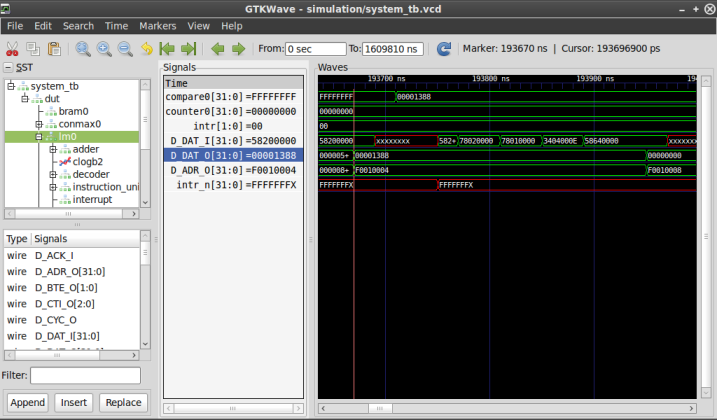
\includegraphics[scale=.7]{./anexo1/images/gtkwave.png}   \end{center}
     \caption{Visualizador de formas de onda \textit{GTKWAVE}} \label{gtkwave}
  \end{figure}

Una vez configurada la FPGA, se utiliza la herramienta \textit{URJTAG} para verificar el correcto funcionamiento del sistema implementado en la FPGA, \textit{URJTAG} proporciona una capa de abstracci�n de hardware que permite el manejo del puerto JTAG de cualquier dispositivo, proporcionando funciones de alto nivel para la aplicaci�n de las funciones JTAG (IDCODE, INTEST, EXTEST, BYPASS, SAMPLE/PRELOAD) permitiendo la aplicaci�n de vectores de prueba al n�cleo l�gico de la FPGA y la captura de la respuesta a estos est�mulos; estas pruebas se realizan a baja frecuencia. \textit{URJTAG} soporta varias interfaces f�sicas para control de las se�ales del puerto JTAG (TDI, TDO, TMS y TCK) las cuales pueden ser conectadas a diferentes puertos de un computador, o como en este caso a un puerto virtual creado en el procesador MIPS.  


\subsubsection{Herramientas para la configuraci�n de PLDs}
Aunque con la plataforma de desarrollo SIE no es necesario utilizar herramientas ni unidades de programaci�n adicionales para configurar su FPGA; el procesador de SIE ejecuta dos aplicaciones que son utilizadas para realizar esta funci�n y pueden ser ejecutadas en computadores personales: \textit{URJTAG} y \textit{XC3SPROG}, las dos funcionan de forma similar, utilizan dispositivos conectados al puerto paralelo (conexi�n directa) o USB (basados en el protocolo MPSSE del chip FT2232) del computador; para ejecutar las instrucciones extendidas de la FPGA CFG\_OUT, CFG\_IN, JSTART y JPROGRAM (hasta el momento solo han sido probadas con las FPGAs de Xilinx).



%%%%%%%%%%%%%%%%%%%%% %%%%%%%%%%% %%%%%%%%%%%%%%%%%%%%%%%%%%%%%%%%%
%
% This section is intended to provide a review on how to use the 
% Programming interfaces
%
%%%%%%%%%%%%%%%%%%%%%%%% %%%%%%%%%%%%%%% %%%%%%%%%%%%%%%%%%%%%%%%%%

\subsection{Interfaz JTAG}
A mediados de los 70s, la estructura de pruebas para tarjetas de circuito impreso (PCB, Printed Circuit Boards) se basaba en el uso de la t�cnica ``bed-of-nails''. Este m�todo utilizaba un dispositivo que conten�a una gran cantidad de puntos de prueba, que permit�an el acceso a dispositivos en la tarjeta a trav�s de puntos colocados en la capa de cobre para dicho fin. Las pruebas se realizaban en dos fases: con el circuito apagado y con el circuito funcionando. Con la aparici�n de los dispositivos de montaje superficial se empez� a colocar dispositivos en las dos caras de la tarjeta, y se redujeron de forma considerable las dimensiones de los dispositivos, disminuyendo la distancia f�sica entre las interconexiones (0.4 - 1mm), dificultando el proceso de pruebas tradicional.

A mediados de los 80s un grupo de ingenieros de pruebas miembros de compa��as electr�nicas europeas se reunieron para examinar el problema y buscar posibles soluciones. Este grupo se auto-denomin� JETAG (Joint European Test Action Group). El m�todo de soluci�n propuesto por ellos estaba basado en el concepto de un registro de corrimiento serial colocado alrededor de la frontera dispositivo, de aqu� el nombre ``Boundary Scan''. Despu�s el grupo se asoci� a compa��as norteamericanas y la ``E'' de ``European'' desapareci� del nombre de la organizaci�n convirti�ndose en JTAG (Join Test Action Group).

\subsubsection{Arquitectura BOUNDARY SCAN} 
A cada se�al de entrada o salida se le adiciona un elemento de memoria multi-prop�sito llamado ``Boundary Scan Cell'' (BSC). Las celdas conectadas a los pines de entrada reciben el nombre de ``Celdas de entrada'', y las que est�n conectadas a los pines de salida ``Celdas de salida''. En la Figura \ref{jtag_basics} se muestra esta arquitectura.

\begin{figure}[h]
  \begin{center} 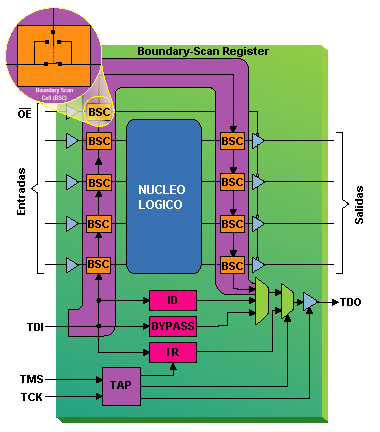
\includegraphics[scale=.6]{./anexo1/images/jtag_basics} \end{center}
  \caption{Arquitectura Boundary Scan} \label{jtag_basics}
\end{figure}

Las BSC se configuran en un registro de corrimiento de entrada y salida paralela. Una carga paralela de los registros (captura) ocasiona que los valores de las se�ales aplicadas a los pines del dispositivo pasen a las celdas de entrada y que opcionalmente los valores de las se�ales internas del dispositivo pasen a las celdas de salida. Una descarga paralela (Actualizaci�n) ocasiona que los valores presentes en las celdas de salida pasen a los pines del dispositivo, y opcionalmente los valores almacenados en las celdas de entrada pasen al interior del dispositivo.

Los datos pueden ser corridos a trav�s del registro de corrimiento de forma serial, empezando por un pin dedicado TDI (Test Data In) y terminando en un pin de salida dedicado llamado TDO (Test Data Out). La se�al de reloj se proporciona por un pin externo TCLK (Test Clock) y el modo de operaci�n se controla por la se�al TMS (Test Mode Select). Los elementos del Boundary Scan no afectan el funcionamiento del dispositivo. Y son independientes del n�cleo l�gico del mismo.

\subsubsection{Instrucciones JTAG}
El Standard IEEE 1149.1 describe tres instrucciones obligatorias: Bypass, Sample/Preload, y Extest \cite{TI96}.

\begin{itemize}
  \item \textbf{BYPASS} Esta instrucci�n permite que el chip permanezca en un modo funcional, hace que el registro de Bypass se coloque entre TDI y TDO; permitiendo la transferencia serial de datos a trav�s del circuito integrado desde TDI hacia TDO sin afectar la operaci�n. La codificaci�n en binario para esta instrucci�n debe ser con todos sus bits en uno. 
  
  \item \textbf{SAMPLE/PRELOAD} Esta instrucci�n selecciona coloca el registro Boundary-Scan entre los terminales TDI y TDO. Durante esta instrucci�n, se puede acceder al registro Boundary-Scan y obtener una muestra de los datos de entrada y salida del chip a trav�s de la operaci�n \textit{Data Scan}. Esta instrucci�n tambi�n se utiliza para precargar los datos de prueba en el registro Boundary-Scan, antes de ejecutar la instrucci�n EXTEST. La codificaci�n de esta instrucci�n la define el fabricante.

  \item \textbf{EXTEST} Esta instrucci�n coloca al circuito integrado en modo de test externo (pruebas de interconexi�n) y conecta el regsitro Boundary-Scan entre TDI y TDO. Las se�ales que salen del circuito son cargadas en el registro boundary-scan en el flanco de bajada de TCK del estado Capture-DR; las se�ales de entrada al dispositivo son cargadas al registro boundary-scan durante el flanco de bajada de TCK dl estado Update-DR (ver Figura \ref{jtag_sm}). La codificaci�n para esta instrucci�n est� definida con todos sus bits en cero.
  
  \item \textbf{INTEST}  La instrucci�n INTEST (opcional) selecciona el registro boundary-scan, pero es utilizado para capturar las se�ales que salen del n�cleo l�gico del dispositivo, y para aplicar valores conocidos a las se�ales de entrada del n�cleo. La codificaci�n para esta se�al es asignada por el dise�ador.
\end{itemize}

\begin{figure}[h]
  \begin{center} 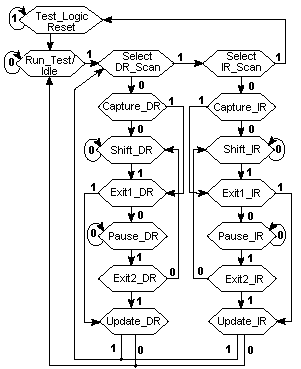
\includegraphics[scale=.8]{./anexo1/images/jtag_sm} \end{center}
  \caption{Arquitectura Boundary Scan} \label{jtag_sm}
\end{figure}



\section{Glosario}
ELF
Objetos
fuentes

binarios
target
reglas
prerequisitos
hdl
codise�o
GNU
GPL
licencias

\section{bib}
No olvidar colocar
Manual del Make tomado de la pagina de GNU project
Managing Projects with GNU Make

\end{document}
